%!TEX root = thesis.tex
\chapter{Active nematics on the surface of a torus}\label{c:3}
\section{Introduction}
Active materials are composed of constituent particles that each can convert stored internal energy, or ambient energy, into work.
As a result, they are intrinsically out of equilibrium~\cite{RN237,RN238,RN40}.
Due to being out of equilibrium, the system is athermal and cannot be understood within the framework of equilibrium statistical mechanics.
However, the constituent particles in active materials are still in motion, similar to the particles in thermal systems.
This is in contrast to passive athermal materials like jammed or granular systems, where individual particles are static.
As a consequence, active materials can exhibit a wide range of emergent phenomena.
Examples include flocking transitions, observed in groups of starlings~\cite{RN239,RN240}; elastic behavior, observed in colonies of fire-ants~\cite{RN242}; and ``superfluid-like'' behavior, observed in bacterial suspensions~\cite{RN270,RN271}.
% ; and crystallization at low volume fraction, observed in self-propelled colloidal particles~\cite{RN168,RN38}.
Within the current theoretical framework of ``active matter,'' the emergent phenomenology is typically governed by a single control parameter called the ``activity''~\cite{RN237,RN238,RN40}.
For example, in the starlings and bacterial suspensions, the activity is associated to the speed of the individual particles; the flocking and superfluid-like behavior only exists for nonzero average velocity.
When the particle speed is zero, both the starlings and the bacteria become passive athermal materials.
Activity is in general defined differently for different systems, with the only requirement being that the passive state corresponds to zero activity.

Note that active materials can be composed of individual units of any size, provided the activity is strong enough.
In fact, the previous examples span 4 orders of magnitude in size, from the starlings at $\mathcal{O}(10^{-1})$ m to the bacteria at $\mathcal{O}(10^{-5})$ m, with their respective behavior all understood within the same framework of ``active matter.''
However, despite the fact that the strength of the activity typically governs the system-wide behavior, there is still no general \emph{a priori} understanding of how adding activity to a passive system will affect its properties and behavior.
Here, we consider how activity affects the interplay between nematic order, geometry, and topology.
\begin{figure}
  \centering
  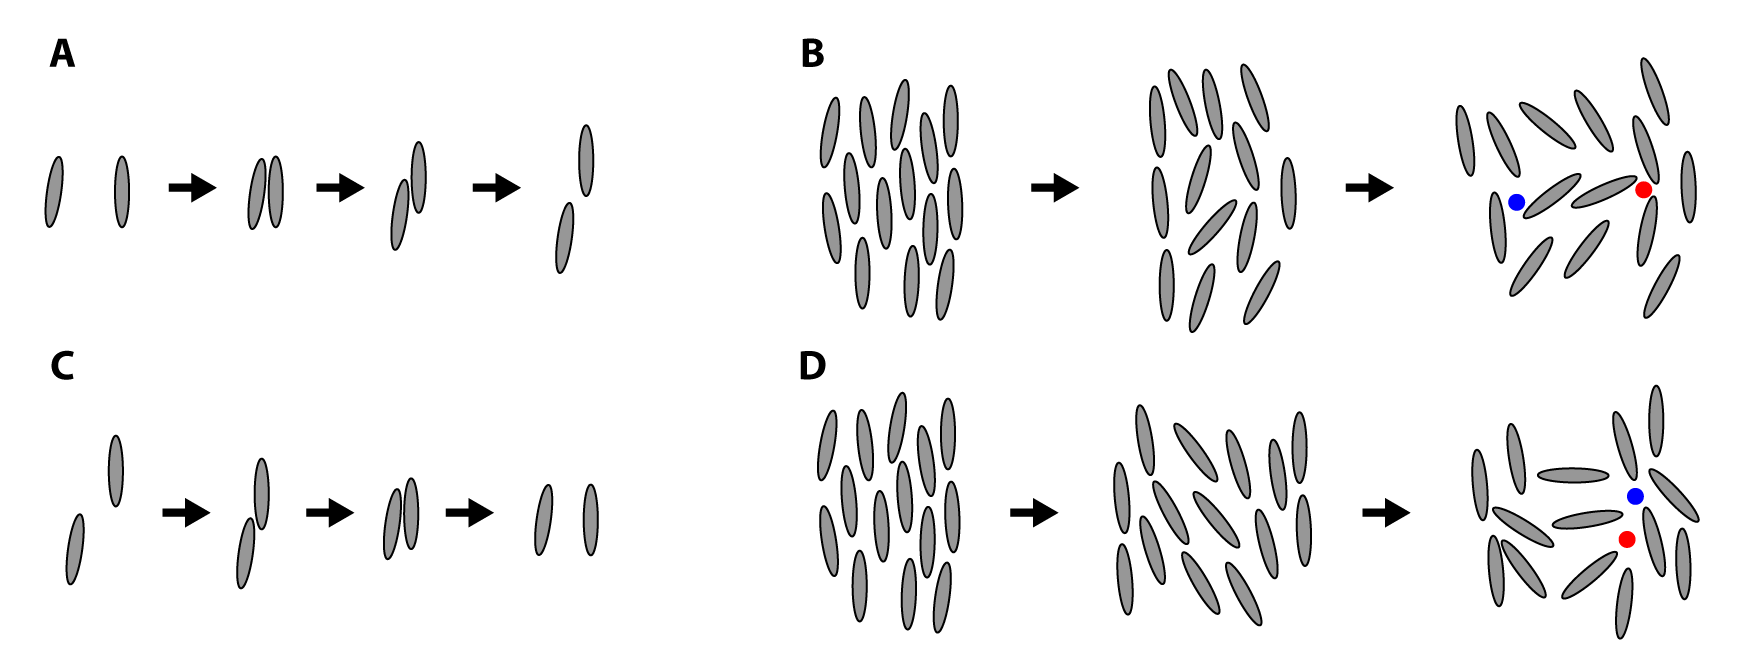
\includegraphics{figures/C3/Ch3-Figs_ActiveInteraction.png}
  \caption{Interactions in extensile and contractile nematics.
  (A,C), Two-particle interaction for extensile (A) and contractile (C) mesogens.
  The arrows represent time.
  (B,D), Active stress exerted on a small area by the surroundings ($\bm{\sigma}$) and on the surroundings by the small area ($\bm{\sigma}'$) for (B) extensile and (D) contractile interactions.
  }\label{f:3-ActiveInteraction}
\end{figure}

Much like equilibrium nematics, the individual mesogens of active nematic materials are anisotropic and thus form a nematic phase; however, the addition of activity to nematic order modifies the interaction between the mesogens.
With the exception of bacteria introduced into lyotropic liquid crystals~\cite{RN86}, to date the majority of experimental and theoretical work on active nematics has taken place in 2D.
Thus, we will highlight the effect of activity on a nematic in 2D.
Consider a pair of active rod-like particles in 2D.
If the active nematic is ``extensile,'' when the two rods touch they will slide past each other and then separate, as illustrated in Figure~\ref{f:3-ActiveInteraction}(A); however, if the active nematic is ``contractile,'' when two rods touch they will slide towards each other and then separate, as illustrated in Figure~\ref{f:3-ActiveInteraction}(C).
\begin{figure}
  \centering
  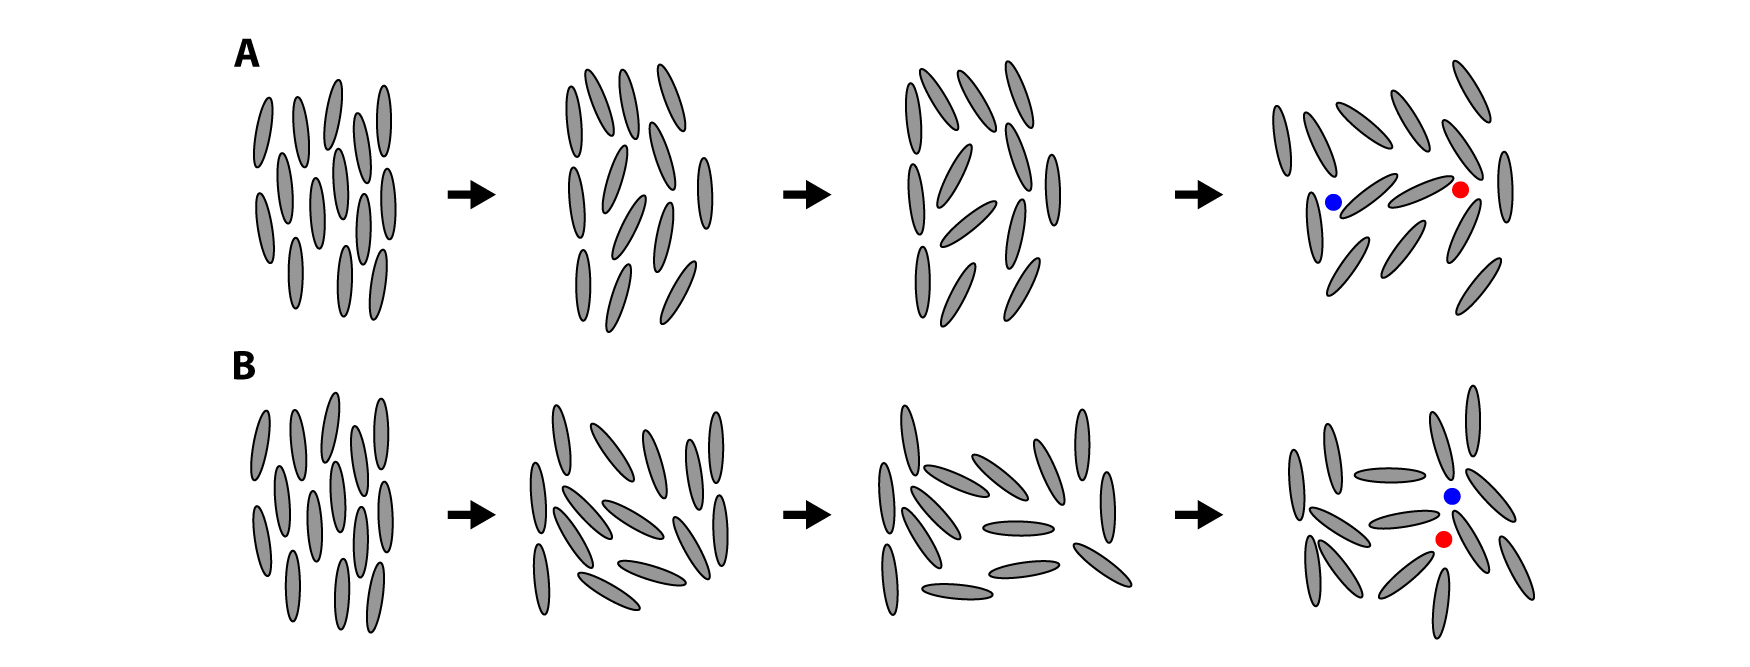
\includegraphics{figures/C3/Ch3-Figs_ActiveDefectGen.png}
  \caption{Activity generates defect pairs.
  An (A) extensile and (B) contractile active nematic evolving over time.
  In both cases a $s = \pm 1/2$ defect pair is generated, with the defects indicated by (${\color{red} \bullet}$), and (${\color{blue} \bullet}$), respectively.}\label{f:3-ActiveDefectGen}
\end{figure}

We can also think about the effect of these interactions at the continuum level; considering the forces from the surrounding material acting on a small area of the nematic and enforcing conservation of momentum, we arrive at the Cauchy momentum equation:
\begin{equation}
  \rho \frac{\textrm{D} \mathbf{v}}{\textrm{D}t } = \nabla \cdot \bm{\tau},\label{e:3-Cauchy}
\end{equation}
where $\textrm{D}/\textrm{D}t = \partial/\partial t + \mathbf{v} \cdot \nabla$ is the material derivative, $\mathbf{v}$ is the fluid velocity, and $\bm{\tau}$ is the stress tensor.
We can rewrite $\nabla \cdot \bm{\tau}$ in Eq.~\ref{e:3-Cauchy} for an incompressible active nematic fluid in terms of the viscosity, $\eta$, the pressure, $p$, the stress from the nematic elasticity $\bm{\sigma}^{elastic}$, and the stress from the activity $\bm{\sigma}^{active}$, yielding:
\begin{equation}
  \rho \frac{\textrm{D} \mathbf{v}}{\textrm{D}t } = \eta \nabla^2 \mathbf{v} - \nabla p + \nabla \cdot \bm{\sigma}^{elastic} + \nabla \cdot \bm{\sigma}^{active}.\label{e:3-NavierStokes}
\end{equation}

Since the active forces act along the director, we can write $\bm{\sigma}^{active} = \alpha \mathbf{Q}$, where $\mathbf{Q}$ is the 2D nematic tensor order parameter defined in Eq.~\ref{e:2-2DOrderDiag}.
If $\mathbf{n} \parallel \hat{e}_1$, with $\{\hat{e}_1,\hat{e}_2 \}$ the standard orthonormal basis, then the active stress becomes
\begin{equation}
  \bm{\sigma}^{active} = \alpha S
  \begin{pmatrix}
    1/2 & 0 \\ 0 & -1/2
  \end{pmatrix}.
\end{equation}
Then, if $\alpha < 0$, $\sigma_{11}^{active} = - |\alpha|S/2 < |\alpha|S/2 = \sigma_{22}^{active}$, as illustrated by the black arrows in Figure~\ref{f:3-ActiveInteraction}(B).
Similarly, if  $\alpha > 0$, $\sigma_{22}^{active} = - |\alpha|S/2 < |\alpha|S/2 = \sigma_{11}^{active}$ [black arrows, Figure~\ref{f:3-ActiveInteraction}(D)].
However, these stresses represent the active stresses of the surrounding material on the area of interest; the active stress due to the area of interest, $\bm{\sigma}'^{active}$, will have the opposite sign.
This is illustrated by the red arrows in Figure~\ref{f:3-ActiveInteraction}(B,D).
When $\alpha < 0$, [Figure~\ref{f:3-ActiveInteraction}(B)] the activity works to extend the nematic along the director, while when $\alpha > 0$ [Figure~\ref{f:3-ActiveInteraction}(C)], the activity works to contract the nematic along the director.
Hence, extensile interactions have $\alpha < 0$ while contractile interactions have $\alpha > 0$~\cite{RN11}.

To further see the ramifications of the activity, we evaluate $\nabla \cdot \bm{\sigma}^{active}$,
\begin{align}
  \partial_j \sigma^{active}_{ij} &= \alpha \partial_j \big(S(n_in_j - \delta_{ij}/2)\big)\label{e:3-ActiveInstabilityA} \\
  &= \alpha(\partial_j S)(n_in_j - \delta_{ij}/2) + \alpha S \big((\partial_j n_i)n_j + n_i(\partial_j n_j) \big) \\
  \nabla \cdot \bm{\sigma}^{active} &= \alpha (\nabla S)^T(\mathbf{n} \otimes \mathbf{n}-\mathbb{1}/2) + \alpha S \big((\mathbf{n} \cdot \nabla)\mathbf{n} + \mathbf{n}(\nabla \cdot \mathbf{n}) \big) \\
  &=  \alpha (\nabla S)^T(\mathbf{n} \otimes \mathbf{n}-\mathbb{1}/2) + \alpha S \big(\mathbf{n}(\nabla \cdot \mathbf{n}) - \mathbf{n} \times \nabla \times \mathbf{n}  \big).\label{e:3-ActiveInstabilityD}
\end{align}
The second term in Eq.~\ref{e:3-ActiveInstabilityD} relates the force density due to the activity to splay and bend distortions in the nematic.
First, consider $\alpha S \mathbf{n}(\nabla \cdot \mathbf{n})$.
The force is always along the director, with the magnitude of the force proportional to the divergence.
Note that the term is symmetric, so regardless of computing the term with $\mathbf{n}$ or $-\mathbf{n}$, the direction of the force is the same; for $\alpha > 0$, the diverging structure will act like a ``source'' and the force will amplify the splay, while for $\alpha < 0$ the diverging structure will act like a ``sink'' and the active force will reduce the splay.
Second, consider $- \alpha S \mathbf{n} \times \nabla \times \mathbf{n}$. Here, the force will be perpendicular to $\mathbf{n}$ and thus work to either amplify ($\alpha < 0$) or suppress ($\alpha > 0$) bend distortions.
In addition, the magnitude of the force is proportional to the magnitude of the bend distortion.
Since the term is symmetric, $\alpha < 0$ will always cause the force to amplify a bend distortion, while $\alpha > 0$ will cause the active force to suppress a bend distortion.

Thus, contractile activity with $\alpha > 0$ amplifies splay distortions and suppresses bend distortions, while extensile activity with $\alpha < 0$ amplifies bend distortions and suppresses splay distortions.
Consequently, if the active stress is greater than the elastic stress,  extensile active nematics are unstable to bend distortions while contractile active nematics are unstable to splay distortions~\cite{RN171,RN170,RN11}.
This instability is illustrated for an extensile and contractile active nematic in Figure~\ref{f:3-ActiveDefectGen}(A,B), respectively, where the instability in both cases eventually results in the creation of an $s=\pm 1/2$ defect pair.

While active nematics can exist in a defect-free state for low activity~\cite{RN247,RN7}, the activity is generally large enough such that the steady-state is often full of pairs of $s = \pm 1/2$ defects that are continuously created and annihilated~\cite{RN11,RN8,RN3,RN27,RN135,RN86}.
Since the active stress acts along the director, the polar structure of the $s = +1/2$ defects will cause these $s = +1/2$ defects to act like self-propelled particles, with the propulsion direction depending on the type of activity~\cite{RN11,RN8}.
For example, consider the director structure of an $s = +1/2$ defect shown by the white lines in Figure~\ref{f:3-DefectFlow}(A); an extensile stress along the director will cause the bend distortion to grow and the splay distortion to decrease, causing the defect to propagate along the red arrow.
In contrast, the interactions in a contractile nematic will cause the defect to propagate opposite to the red arrow.
However, due to the three-fold symmetry of $s = -1/2$ defects, as shown by the white lines in Figure~\ref{f:3-DefectFlow}(B), any stress along the director will have no effect on the defect position.
Thus, $s = -1/2$ defects are not driven by the activity and instead are only advected by interactions between the defects.
As a consequence, the dynamics in an active nematic are driven only by the motion of $s = +1/2$ defects~\cite{RN7}.
\begin{figure}
  \centering
  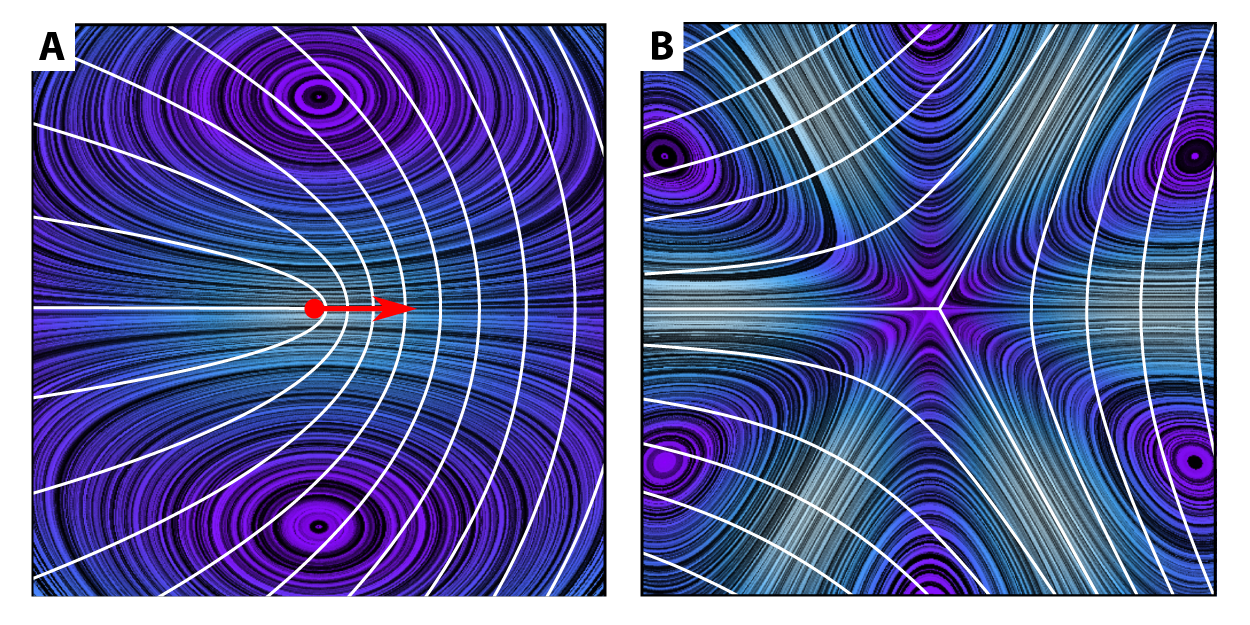
\includegraphics{figures/C3/Ch3-Figs_DefectFlow.png}
  \caption{Flow fields for active disclinations.
  (A,B) Flows generated by active (A) and $s=+1/2$ and (B) $s=-1/2$ disclinations, with the director lines drawn in white.
  Due to the polar structure of the active flow, $s = +1/2$ disclinations propel along their symmetry axis.
  The red arrow represents the propulsion direction for an extensile nematic; $s = +1/2$ disclinations will propel in the opposite direction for a contractile nematic.}\label{f:3-DefectFlow}
\end{figure}

Recent experimental studies with active nematics yielding self-regulated behaviors such as self-sustained oscillations~\cite{RN9}, spontaneous formation of morphological features such as kinks and protrusions~\cite{RN9,RN3}, and undirected motility~\cite{RN9,RN3} have acted as stimulus to investigate how biological functionality emerges from the interplay between activity, the geometry of the system, and the structure of the internal phase~\cite{RN160,RN51,RN10}.
In this context, defects in active nematics could be harnessed to achieve life-like functionality, as defects are extremely sensitive to the intrinsic curvature of the space they inhabit.
This is illustrated in Eq.~\ref{e:1-TopTheoryofDefects}, where topological defects on a surface are treated like point charges interacting among themselves and with a background charge density provided by the Gaussian curvature of the surface.

However, despite theoretical interest in the interplay between varying Gaussian curvature and topological defects, with few exceptions~\cite{RN84,RN25,RN73,RN81}, there has been little experimental work with defects on surfaces where the Gaussian curvature is non-constant.
More notably, there has been no experimental work where the defects have the option to explore regions with both positive and negative Gaussian curvature.

In this latter scenario with nematic order, the topological charge is expected to unbind; starting with an $s = \pm 1/2$ defect pair, the $s = +1/2$ defect will migrate to a region of positive Gaussian curvature, while the $s=  -1/2$ defect will instead migrate to a region of negative Gaussian curvature~\cite{RN17,RN19,RN22}.
For example, consider the schematic of a torus in Figure~\ref{f:3-EqDefs}(A) with the $K>0$ region in red and the $K<0$ region in blue.
For a torus specified by a central ring radius, $R_0$, and a tube radius, $a$, we use the toroidal coordinates $\{r,\theta,\varphi\}$, with $\{r,\theta \}$ the usual polar coordinates in the circular cross section and $\varphi$ the azimuthal angle [see Figure~\ref{f:3-EqDefs}(B)].
We define the aspect ratio of the torus as $\xi = R_0/a$.
For low $\xi$, the ground state of a nematic on a torus is predicted to have defects due the ability of the defects to ``screen'' the Gaussian curvature of the surface.
Specifically, introducing 4 pairs of $s = \pm 1/2$ defects onto the surface, as depicted in Figure~\ref{f:3-EqDefs}(A), completely screens the Gaussian curvature of the surface.
We see that the $s = +1/2$ defects are predicted to minimize their energy when they are located on the outside of the ``hole,'' thereby screening the positive Gaussian curvature, and the $s = -1/2$ defects are predicted to sit on the inside of the ``hole'' to screen the negative Gaussian curvature.
The repulsion between the like-signed defects cause the defects to be spaced in intervals of $\varphi = \pi/2$; increasing the repulsion can lead to fewer than 4 pairs of defects as the ground state.
In addition, the ground state is only predicted to be defective when the curvature is large enough to overcome the attraction between opposite-signed defects.

For the schematic in Figure~\ref{f:3-EqDefs}(A), if we integrate over the red $K>0$ region where $\theta \in [\pi/2,3 \pi/2]$, and consider $\varphi \in [0,\varphi']$, we can compare the integral as a function of $\varphi'$ with the net topological charge in the region.
Since both of these quantities depend on $\varphi'$, we get the parametric curve depicted in red in Figure~\ref{f:3-EqDefs}(C).
Similarly, integrating over the blue $K<0$ region defined by $\theta \in [-\pi/2,\pi/2]$ as a function of $\varphi'$ and comparing with the net topological charge in the region yields the parametric curve depicted in blue in Figure~\ref{f:3-EqDefs}(C).
We see that the curves in Figure~\ref{f:3-EqDefs}(C) have positive slopes, indicating the curvature-induced defect unbinding, and the curves are stepped, reflecting the discrete nature of the topological charge.
Recall for nematics in 2D, the topological charge occurs in quanta of $1/2$.
In addition, note that the total integrated Gaussian curvature in the $K>0$ region and the $K<0$ region is $+4 \pi$ and $-4\pi$, respectively.
Since each $s = \pm 1/2$ defect corresponds to a $\pi$ rotation of $\mathbf{n}$, the four pairs of defects on the torus exactly screens the total integrated $K$ of the $K > 0$ and $K<0$ regions.
\begin{figure}
  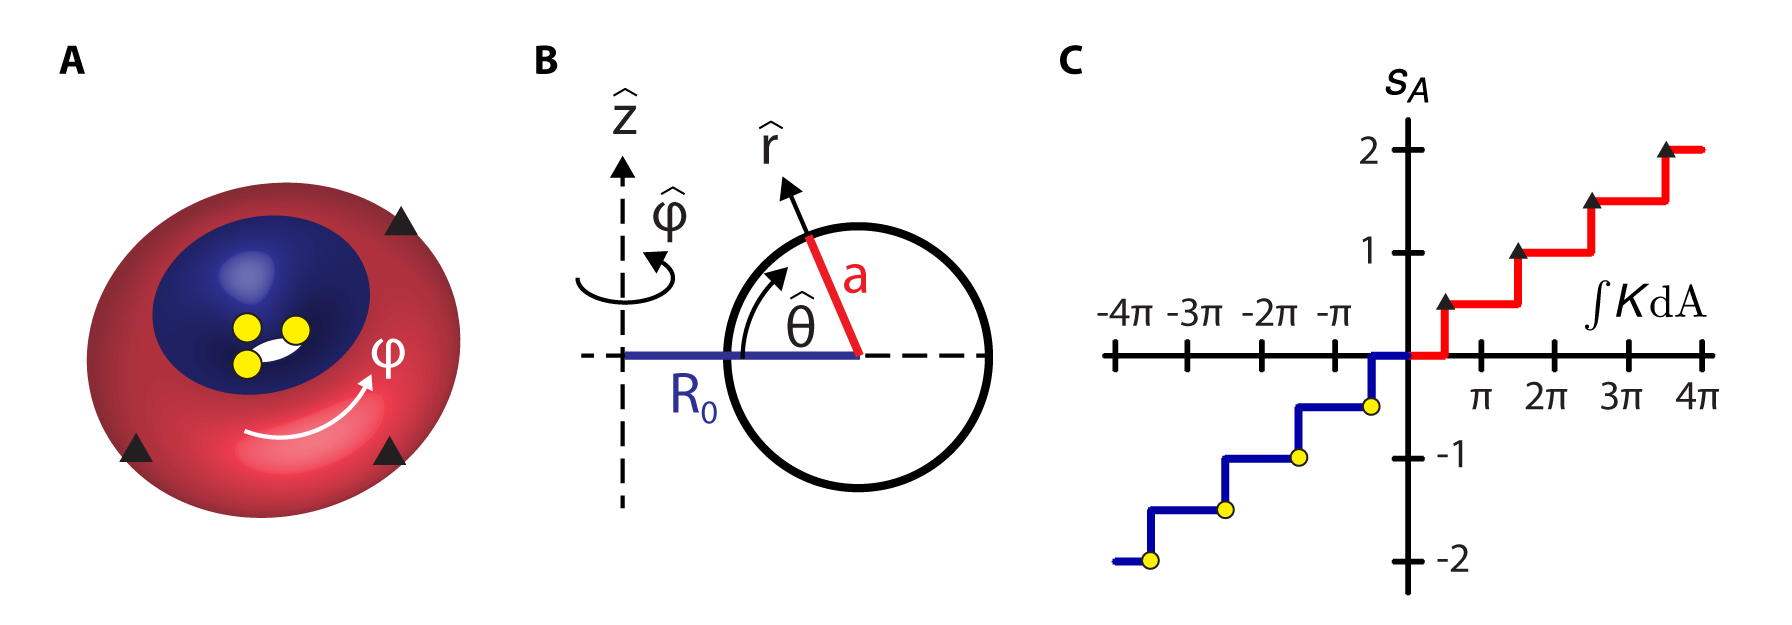
\includegraphics{figures/C3/Ch3-Figs_EqDefs.png}
  \caption{Curvature-induced defect unbinding for a nematic on a torus. (A) A schematic of a torus with 4 pairs of unbound pairs of $s = \pm 1/2$ defects. The 3 visible $s=+1/2$ defects are indicated by $\blacktriangle$ and the 3 visible $s = -1/2$ defects are indicated by ${\color{yellow} \bullet}$.
  The red region on the torus has $K >0$ and the blue region has $K<0$.
  (B) A schematic of a cross-section of a torus defining the toroidal coordinate system $\{r, \theta, \varphi \}$.
  A given torus is specified by its central circle radius, $R_0$ and its tube radius, $a$, which combine to form the aspect ratio, $\xi = R_0/a$.
  (C) Plot of topological charge vs integrated Gaussian curvature as $\varphi$ increases for the torus in (A).
  The red curve corresponds to integrating over the red region defined by $\theta \in [\pi/2,3 \pi/2]$ and the blue curve corresponds to integrating over the blue region defined by $\theta \in [-\pi/2,\pi/2]$. The positive slope indicates defect unbinding.}\label{f:3-EqDefs}
\end{figure}

In this chapter, we address this situation experimentally using a 2D extensile active nematic on the surface of a toroidal droplet.
The active nematic is composed of microtubules driven by kinesin motors and fueled by adenosine triphosphate (ATP); the strength of the activity in this material is tuned by the ATP concentration, with higher ATP concentrations causing the kinesin motors to introduce more kinetic energy into the system.
Since the torus has a handle, it has a genus of one and thus according to the Poincar\'e-Hopf Theorem written in Eq.~\ref{e:1-PH}, the nematic field must have zero net topological charge.
In our experiments, the activity is large enough such that the torus is always populated with a sea of constantly moving $s = \pm 1/2$ defects that are dynamically created and annihilated.
The topological constraints, nevertheless, force the number of $s = +1/2$ defects to be equal to the number of $s = -1.2$ defects.

Interestingly, despite the nonequilibrium dynamics of the defects, we find that on average, pairs of $s = \pm 1/2$ topological defects unbind, with the individual defects migrating to regions with like-signed Gaussian curvature.
However, as a result of the averaging process in our analysis, the average topological charge in a region on the surface ceases to take on discrete values and instead becomes a continuous variable.
In addition, contrary to expectations from equilibrium predictions~\cite{RN36,RN19,RN22,RN20,RN78}, we find that this active unbinding depends only on the local geometry and that it is independent of the system size and aspect ratio.

Our studies are performed with two different ATP concentrations and thus two different levels of activity.
We find that the unbinding depends on activity.
In addition, we characterize the defect number fluctuations in a region on the surface and find that the relative root-mean-squared (RMS) defect number fluctuations is inversely proportional to the square root of the average number of defects in the region.
Interestingly this is the expected result for an equilibrium system of particles subject to number fluctuations.
A numerical integration of the equation of motion of active nematic defects~\cite{RN11,RN8,RN9} performed by Luca Giomi and Dan Pearce at the University of Leiden confirms our experimental results and indicates that the defect unbinding depends on the defect number density and that the unbinding can be suppressed in the limit of high activity.
Furthermore, by using topological defects as micro-rheological tracers and quantitatively comparing our experimental and theoretical results, we are able to estimate the Frank elastic constant, the active stress $\alpha$, and the defect mobility of a microtubule-kinesin active nematic liquid crystal for the first time.
Overall, our results not only confirm the theory of topological defects on curved surfaces, but also demonstrate the interesting phenomenology that arises from adding activity to the interplay between geometry, topology, and order.
Our work thus provides insights into the physics of partially ordered active matter and introduces a new avenue for the quantitative mechanical characterization of active fluids.


\section{Making active nematic toroids}
\subsection{Active nematic formulation}
We use the mictotubule-kinesin active nematic system pioneered by the Dogic Group at Brandeis University as published in references~\cite{RN3,RN27,RN9,RN135,RN134}.
Microtubules are long, hollow rods that self-assemble from dimers of the $\alpha$-- and $\beta$--tubulin proteins~\cite{RN248}.
The $\alpha$/$\beta$--tubulin dimers polymerize end-to-end to form long chains that then assemble laterally to create cylindrical structures with a helical wrapping of $\alpha$-- and $\beta$--tubulin chains~\cite{RN248,RN249}, as depicted schematically in Figure~\ref{f:3-ActiveBuild}.
This structure gives microtubules a polarity with the (+) end associated with the unpolymerized $\beta$--tubulin subunits and the (-) end associated with the unpolymerized $\alpha$--tubulin subunits~\cite{RN248,RN249}.

While the microtubules serve as the mesogens of the active nematic, the activity comes from kinesin motor proteins bound in clusters to a streptavidin protein.
When in contact with a microtubule, kinesin ``walks'' along the microtubule in discrete steps from the (-) end towards the (+) end, hydrolyzing one ATP molecule into an adenosinediphosphate (ADP) molecule for every 8-nm step~\cite{RN250}.
Thus, a kinesin cluster in contact with two antiparallel microtubules will induce a sliding motion due to the motion of the kinesin motors that will displace the two microtubules in opposite directions~\cite{RN4,RN3}.
Conversely, a kinesin cluster in contact with two parallel microtubules will simply walk along both microtubules in the same direction and thus induce no relative motion between the microtubules~\cite{RN4,RN3}.
These two scenarios are illustrated schematically in Figure~\ref{f:3-ActiveBuild}(B).
\begin{figure}
  \centering
  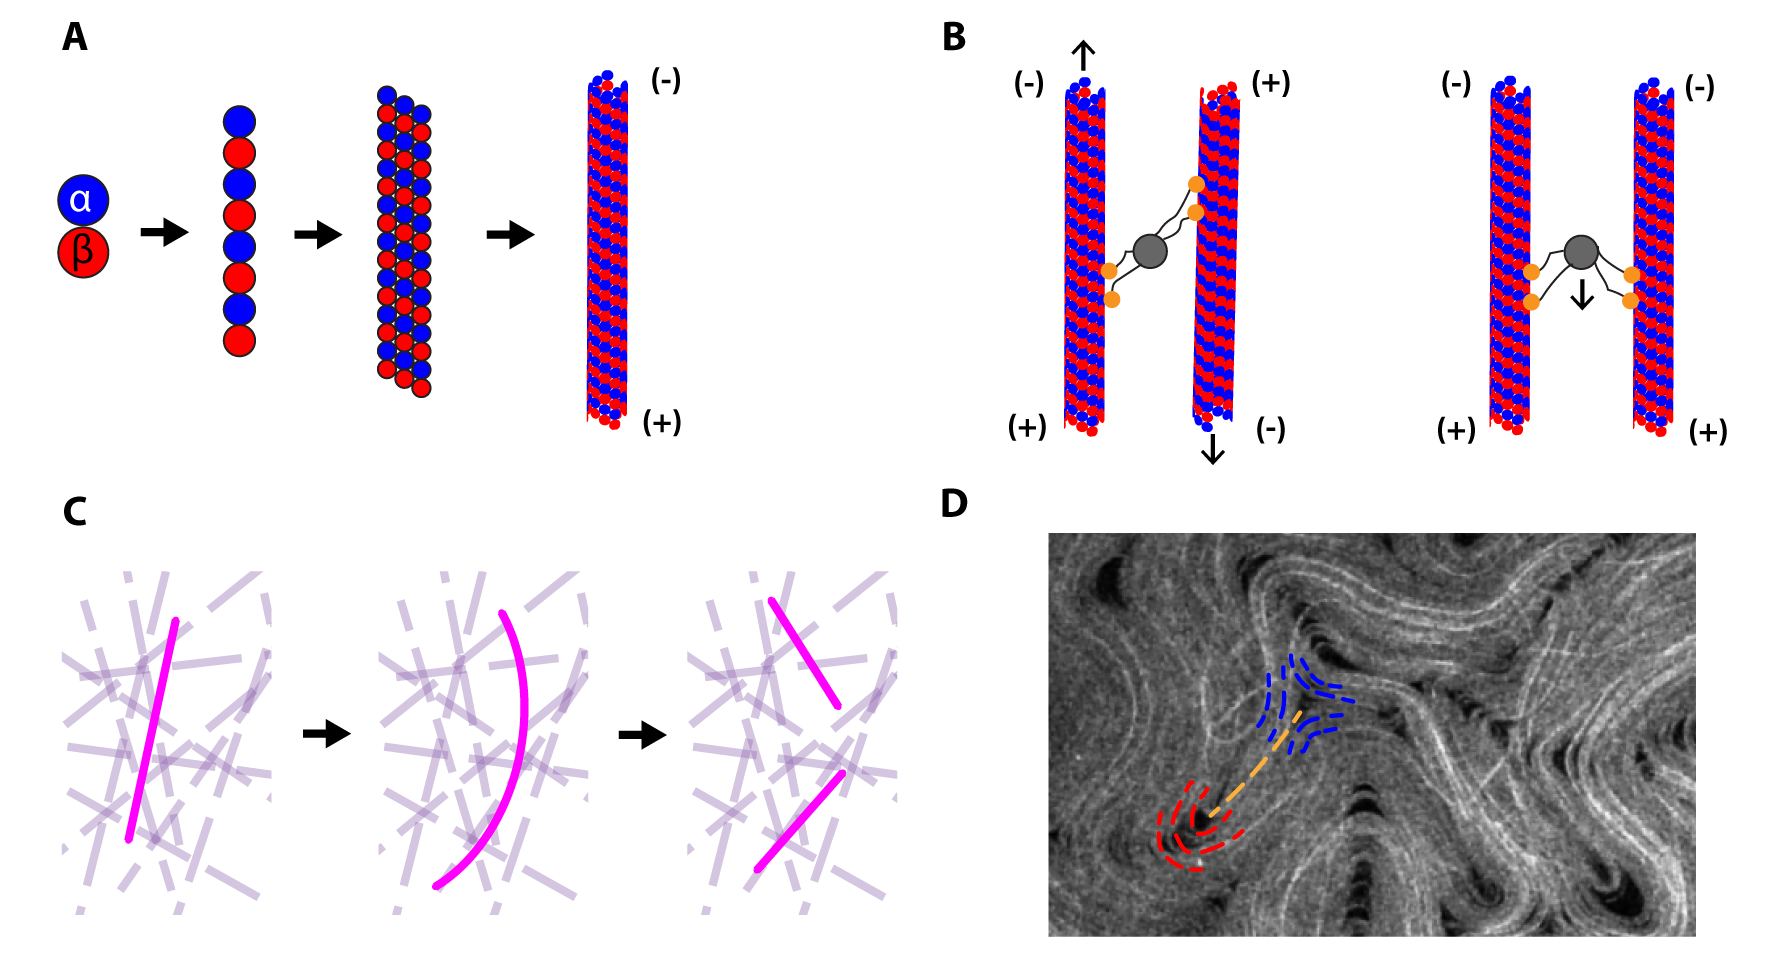
\includegraphics{figures/C3/Ch3-Figs_ActiveBuild.png}
  \caption{Microtuble-kinesin active nematic liquid crystal.
  (A) Schematic of tubulin polymerizing into a microtubule. The $\alpha/\beta$-tubulin dimers polymerize end-to-end to form chains which then polymerize laterally to form microtubules.
  The microtubule polarity is indicated on the schematic, with (-) associated to free $\alpha$-tubulin and (+) associated to free $\beta$-tubulin.
  (B) Kinesin $({\color{yellow} \bullet})$ walks along microtubules from the (-) end to the (+) end.
  When kinesin are bound to streptavidin $({\color{gray} \bullet})$ to form clusters, these clusters can generate relative motion between two antiparallel microtubules.
  In contrast, parallel microtubules exhibit no relative motion, with the kinesin-streptavadin cluster simply translating itself in the shared (+) direction.
  (C) Microtubules and kinesin-streptavidin clusters bundles together by depletion form fibers that slide past each other.
  When the concentration of fibers is high enough to form a viscoelastic network, individual fibers cannot slide freely and instead will buckle and fracture.
  (D) In the presence of a liquid-liquid interface, the fibers will deplete to the interface and undergo an isotropic-nematic transition, with the fiber direction giving the nematic director.
  Pictured is a fluorescence microscopy snapshot of an active nematic, where the microtubules are fluorescently labeled such that the fiber direction is apparent.
  The director surrounding an $s = + 1/2$ and $s = -1/2$ defect pair is highlighted by the dashed red and blue lines, respectively, with the fracture line connecting the pair highlighted with a yellow dashed line.}\label{f:3-ActiveBuild}
\end{figure}

Apart from the activity provided by the kinesin motors, the microtubules in solution interact via the depletion interaction~\cite{RN251}, which is introduced by the presence of poly(ethylene glycol) (PEG, 20 kDa) as a depletant.
The depletion interaction ``bundles'' the microtubules together to form filaments that continuously slide past each other due to the extensile interaction exerted by the kinesin motors~\cite{RN244,RN4,RN3}.
In 3D, when the concentration of filaments in the solution is large enough, the filaments form a viscoelastic network~\cite{RN253,RN3}.
This network inhibits the sliding motion of the filaments such that they eventually buckle at a critical length scale~\cite{RN253,RN3} and fracture into smaller fragments that subsequently recombine with other filaments, starting the sliding-and-buckling process anew, as illustrated in Figure~\ref{f:3-ActiveBuild}(C).

In the presence of a liquid-liquid interface, the depletion interaction drives the filaments to the interface between the microtubule solution and the outer phase.
As the concentration at the interface increases, the filaments locally align and undergo a transition to the nematic phase~\cite{RN3,RN135,RN134}, as seen in the example fluorescence microscopy image in Figure~\ref{f:3-ActiveBuild}(D), where the microtubules are fluorescently labeled such that the fiber direction is readily apparent.
Thus, the filament direction provides the director for the 2D active nematic at the interface.

We note that the sliding-and-buckling phenomenology of the active filaments is the physical mechanism behind the extensile active stress in the nematic phase; it is directly responsible for the bend instability and associated defect formation in the microtubule-kinesin active nematics.
In the nematic phase, when the filaments buckle and fracture, an $s =  \pm 1/2$ defect pair is produced, with the defects nucleating at opposite ends of the fracture line~\cite{RN3,RN11}, as highlighted by the yellow dashed line in the example image in Figure~\ref{f:3-ActiveBuild}(D).

Microtubules, kinesin-streptavidin complexes (K/SA), ATP, a depletant, and an outer liquid phase constitute the essential ingredients for an active nematic.
However, there are many more compounds in this active nematic solution that serve to enable measurements~\cite{RN3,RN135}, prolong activity~\cite{RN3,RN135}, and allow for the silicone-based outer phase that we use to make our toroidal droplets~\cite{RN135}.
As mentioned earlier and shown in Figure~\ref{f:3-ActiveBuild}(D), the microtubules are fluorescently labeled such that the active nematic can be imaged with fluorescence or fluorescence confocal microscopy.
To prevent the excitation source from damaging the fluorophores (photobleaching) or killing the kinesin motors (phototoxicity), the active solution contains trolox (Sigma, 238813) and two anti-oxidant solutions.
Anti-oxidant solution 1 (AO1) is composed of glucose and dithiothreitol (DTT) and Anti-oxidant solution 2 (AO2) is composed of glucose oxidase (Sigma, 238813) and catalase (Sigma, C40).
The active solution also includes an ATP regeneration system to keep the ATP concentration in an active nematic solution constant.
This system is driven by the enzyme mixture pyruvate kinase/lactate dehydrogenase (PK/LDH, Sigma, P-0294) which consumes phoshoenol pyruvate (PEP) to convert ADP to ATP at a rate faster than the K/SA hydrolyzes ATP to ADP~\cite{RN246}.

We note that when driven to the liquid-liquid interface, the active filaments do not ever contact the outer phase.
Instead, the interface is packed with a suitable surfactant such that the active nematic filaments deplete to the polar portion of the surfactant molecule.
The surfactant is then moved along the interface by the motion of the active filaments such that the viscosity of the outer oil phase significantly affects the dynamics of the active nematic~\cite{RN135}.
For a silicone-based outer fluid, we include the triblock copolymer Pluronic F127 (F127) composed of 2 hydrophilic PEG blocks attached to a central hydrophobic poly(propylene oxide) (PPO) block like PEG-PPO-PEG~\cite{RN252}.
Finally, the solution is buffered using a specially designed microtubule buffer (M2B) to keep the enzymes and the motors in their preferred environments~\cite{RN3}.
\begin{table}
  \centering
  \caption{Stock solutions used to form an active nematic solution. The stock solutions in their given compositions are {\bf bolded}.}
  \begin{tabular}{|l !{---}
                  >{\raggedright\arraybackslash}p{.6\textwidth}|}
    \hline
    {\bf M2B}& 80 mM 1,4-piperazinediethanesulphonic (PIPES) buffer~\cite{RN243} +2 mM MgCl$_2$ + 1mM egtazic acid (EGTA), pH 6.8 \\
    {\bf PEP}& 200 mM in {\bf M2B}, pH 6.8. \\
    {\bf PK/LDH}& Used as purchased. \\
    {\bf ATP}& 50 mM in {\bf M2B}, pH 6.8 \\
    {\bf DTT}& 0.5 mM in {\bf M2B}, pH 6.8 \\
    {\bf trolox}& Used as purchased. \\
    {\bf MIX}& 67 mM MgCl$_2$ in {\bf M2B} \\
    {\bf PEG}& (20 kDa) 6\% w/w in {\bf M2B} \\
    {\bf F127}& 12\% w/w in {\bf M2B} \\
    {\bf glucose}& 300 mg/mL in 20 mM K$_2$HPO$_4$ + 70 mM KCl (pH 7.2) \\
    {\bf glucose oxidase}& 20 mg/mL in 20 mM K$_2$HPO$_4$ (pH 7.5) \\
    {\bf catalase}& 3.5 mg/mL in 20 mM K$_2$HPO$_4$ (pH 7.4) \\
    {\bf K/SA}& 0.175 mg/mL K401 + 0.1 mg/mL streptavidin (Invitrogen, S-888) + 12.5 mM imidazole (pH 6.8) + 1 mM MgCl$_2$ + 0.75 mM DTT + 12.5 mM ATP in {\bf M2B}. K401 consists of 401 amino acids of the N-terminal motor domain of \emph{D.~melanogaster} kinesin purified as previously published~\cite{RN3}. \\
    {\bf MT}& 8 mg/mL tubulin labeled with AlexaFluor 647 at 28\% labeling efficiency in {\bf M2B}. Tubulin was purified as previously published~\cite{RN243}.\\
    \hline
  \end{tabular}\label{t:3-ActiveStock}
\end{table}

For an experiment, we build the active nematic solution from stock solutions per the recipe in Table~\ref{t:3-ActiveStock}.
The stock solutions in their given compositions are {\bf bolded} such that PEP refers to the general compound while {\bf PEP} refers to the stock concentration/formulation as defined in Table~\ref{t:3-ActiveStock} and originally prepared by the Dogic Group at Brandeis.
The stock solutions were  shipped to Georgia Tech, and we pipetted the stock solutions as received into aliquots suitable to make 100 $\upmu$L of active nematic solution.
The aliquots are stored in a freezer at $-80^o$ C to prevent degradation of the active compounds.
Prior to each experiment, we remove a set of aliquots from the freezer, quickly thaw the aliquots to room temperature by holding them in our closed hands, and then place all the aliquots on ice except for the {\bf MT} aliquot.
We leave the {\bf MT} aliquot out at room temperature so that the tubulin can self-assemble into microtubules.
The polymerization of microtubules is temperature-dependent, with tubulin polymerizing to form microtubules at room temperature and microtubules depolymerizing into tubulin at low temperature~\cite{RN3}.

We then make the initial mixtures and the pre-solution according to the recipe in Table~\ref{t:3-recipe}, leaving the pre-solution on ice.
We wait at least 90 minutes after bringing the {\bf MT} aliquot to room temperature before mixing it with the pre-solution to form the final active nematic solution as specified in Table~\ref{t:3-recipe}.
Note that we bring the pre-solution to room temperature before adding in the microtubules such that the microtubules do not depolymerize when they are added to the pre-solution.
Once we mix the final solution together, we perform our experiments and observe the active nematic until activity ceases.
\begin{table}[ht]
  \centering
  \caption{Recipe for 100 $\upmu$L active nematic solution}
  \begin{tabular}{|r l|}
    \hline
    \multicolumn{2}{|c|}{Initial mixtures}\\
    \hline
    A01 & 1.5 $\upmu$L {\bf DTT} + 1.5 $\upmu$L {\bf glucose} \\
    A02 & 1.5 $\upmu$L {\bf glucose oxidase} + 1.5 $\upmu$L {\bf catalase} \\
    ATP2 & 2 $\upmu$L {\bf ATP} in:\\
    & \quad 18 $\upmu$L {\bf M2B} for a 144 $\upmu$M final ATP concentration.\\
    & \quad 38 $\upmu$L {\bf M2B} for a 36 $\upmu$M final ATP concentration.\\
    \hline
    \multicolumn{2}{|c|}{Pre-solution}\\
    \hline
    2.21 $\upmu$L & A01\\
    2.21 $\upmu$L & A02\\
    2.83 $\upmu$L & ATP2\\
    2.83 $\upmu$L & {\bf PK/LDH} \\
    4.83 $\upmu$L & {\bf MIX}\\
    10.00 $\upmu$L & {\bf trolox}\\
    13.33 $\upmu$L & {\bf PEP}\\
    13.33 $\upmu$L & {\bf PEG}\\
    16.67 $\upmu$L & {\bf F127}\\
    6.67 $\upmu$L & {\bf K/SA}\\
    8.40 $\upmu$L & {\bf M2B}\\
    \hline
    \multicolumn{2}{|c|}{Active nematic solution}\\
    \hline
    83.33 $\upmu$L & Pre-solution (full volume is 83.33 $\upmu$L)\\
    16.67 $\upmu$L & {\bf MT}\\
    \hline
  \end{tabular}
  \label{t:3-recipe}
\end{table}


\subsection{Flat sample confirmation}
Upon receiving the stock solutions, we first made a bulk active gel according to the procedures published in Ref.~\cite{RN3} to confirm the integrity of the solutions through the shipping process.
To make an active gel, we have to construct a sample chamber where the depletion interaction cannot drive the bundles to aggregate on the walls of the chamber.
We build the sample chamber from a glass coverslip attached via two-sided tape to a microscope slide to form a rectangular channel, as previously published~\cite{RN3}.
Prior to construction, we coat the coverslip and microscope slide with polyacrylamide brushes according to the published protocol~\cite{RN3}, reproduced in Appendix~\ref{a:B}, such that the PEG can penetrate between the brushes, keeping the depletion interaction from driving the active filaments to the glass surface, where they would adsorb~\cite{RN3}.

To make the rectangular sample chambers from the polyacrylamide-coated glass, we cut strips of 2-sided tape such that they are $\approx1$ mm wide and longer than the coverslip.
We then affix the tape strips to the microscope slide in parallel with $\approx 2$ mm between the edges of adjacent strips, and then stick the coverslip onto the tape to create a parallel series of rectangular channels.
Finally, we fill the channels with the active solution using capillary action and seal the ends of the channel with epoxy (DEVCON, 5-minute).
A schematic of the sample chamber and assembly process is shown in Figure~\ref{f:3-SampleChamber}.
The samples are now ready to be imaged using fluorescence or fluorescence confocal microscopy.
\begin{figure}
  \centering
  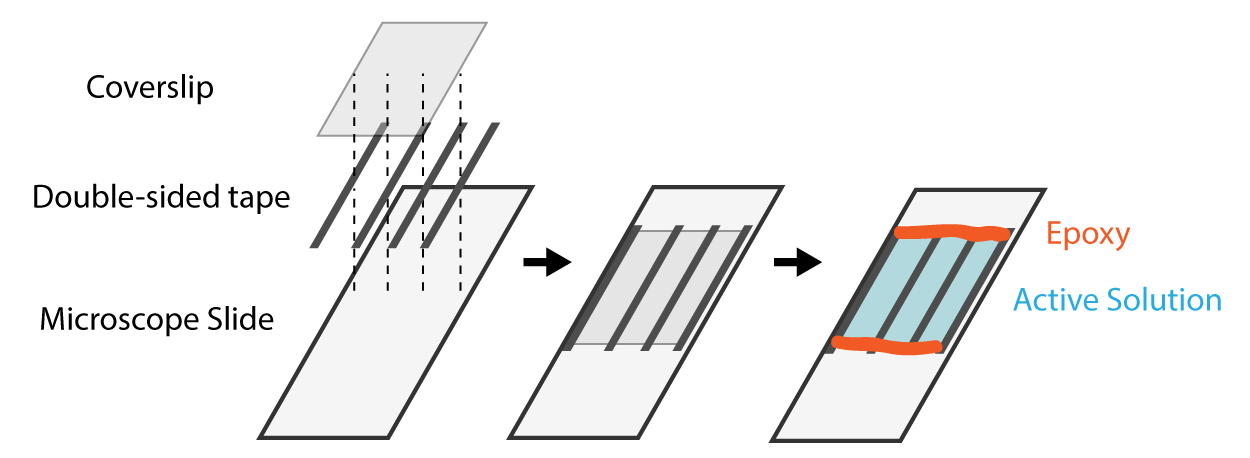
\includegraphics{figures/C3/Ch3-Figs_GelSampleChamber.png}
  \caption{Schematic and assembly of a sample chamber for an active gel.}
  \label{f:3-SampleChamber}
\end{figure}

We confirmed that the stock solutions received produced an active gel with fluorescent active filaments that underwent the sliding/buckling/fracture/recombination cycles.
The activity in the gel sample appeared constant for the entirety of its  $\approx 24$ hr lifespan.
The observed behavior qualitatively agreed with previously published behavior by the Dogic group~\cite{RN3}.


\subsection{Making toroidal droplets}
With the integrity of the active solution confirmed, we turn to making stable toroidal droplets with our active solution.
We generate our toroidal droplets following the procedure detailed in Refs.~\cite{RN29,RN47,RN257}.
The setup consists of a rotating stage holding a cuvette containing the continuous, or outer phase, and a syringe holding the dispersed, or inner phase connected to a needle inserted into the cuvette.
We control the angular velocity of the rotation, $\omega$, by driving the rotating stage with a motor powered by a constant voltage source.
We control the position of the needle in the cuvette with a micromanipulator, and the flow rate and volume of the inner phase with a syringe pump.
In addition, we place a camera below the rotation stage such that we can image the droplet generation process.

This setup is depicted schematically in Figure~\ref{f:3-MakeTorus}(A).
We insert the needle into the cuvette offset from the center of rotation such that pumping the inner phase into the cuvette while the cuvette is rotating will generate a curved jet, as shown in the example image in Figure~\ref{f:3-MakeTorus}(B).
Provided that we rotate fast enough such that the curved jet closes upon itself before it undergoes breakup, we form a toroidal droplet, as shown in the example image in Figure~\ref{f:3-MakeTorus}(C).
This condition is a balance of two timescales: (i) the timescale required to undergo breakup, $t_b \approx \mu_o a_{jet} f(\mu_i/\mu_o)/\gamma$, where $\mu_o$ is the viscosity of the outer phase, $\mu_i$ is the viscosity of the inner phase, $a_{jet}$ is the radius of the jet, $f(\mu_i/\mu_o)$ a function that depends on the viscosity contrast, and $\gamma$ is the interfacial tension between the inner and outer phases;
  and (ii), the timescale required to close the curved jet onto itself, $T = 2\pi/\omega = 2 \pi R_{tip}/U$, where $R_{tip}$ is distance from the center of rotation to the needle, as depicted in Figure~\ref{f:3-MakeTorus}(C), and $U$ is the linear velocity of the continuous phase at the needle.

Equating the two timescales and rearranging terms allows us to express this condition as: $\textup{Ca}_o > (2 \pi / f(\mu_i/\mu_o))R_{tip}/a_{jet}$, where $\textup{Ca}_o = \mu_o U/\gamma$ is a dimensionless group called the Capillary number quantifying the relative importance of the viscous stresses and the stresses due to surface tension.
We note that $a_{jet} \approx a_{tip}$, the radius of the needle.
A jet will thus form at sufficiently high $U$ for given inner and outer materials.
% Experimentally, it has been found that $\textup{Ca}_o > 2.2 R_{tip}/a_{tip}$ for $\mu_o = 5000$~mPa$\cdot$s and $\mu_i = 1$~mPa$\cdot$s in order to form a torus~\cite{RN29}.
To control the size and aspect ratio of the toroidal droplet, we tune $R_0$ by changing $R_{tip}$ while tuning $a$ through the total injected volume.
\begin{figure}
  \centering
  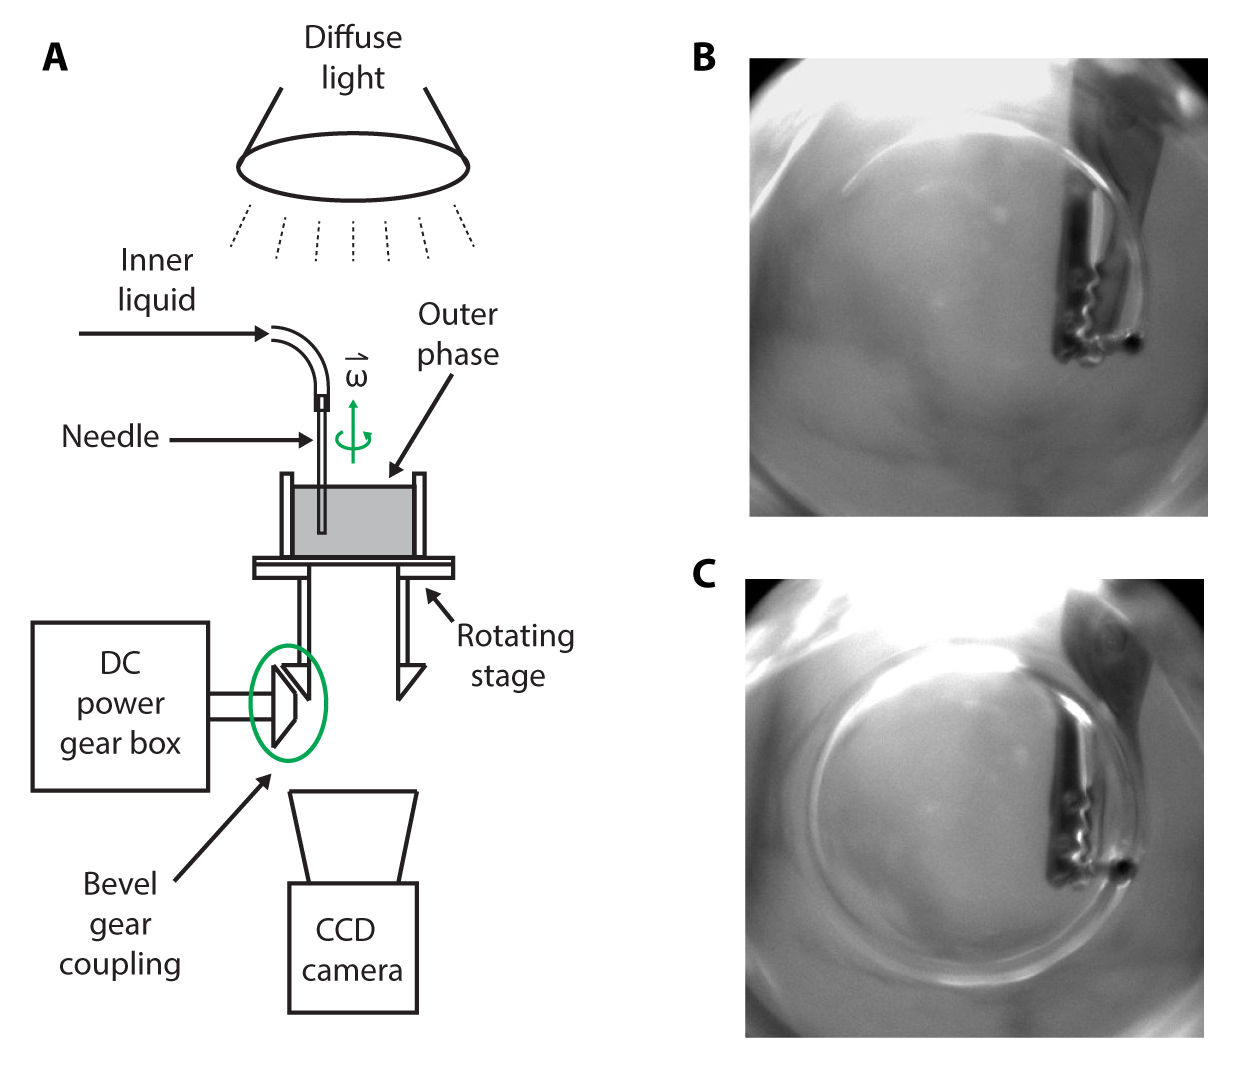
\includegraphics{figures/C3/Ch3-Figs_MakeTorus.png}
  \caption{Making toroidal droplets.
  (A) Schematic of the apparatus used to make toroidal droplets.
  The inner fluid is injected into a cuvette on a rotating stage.
  The stage is driven by a DC motor and the entire process is imaged from below with a CCD camera.
  (B) A curved jet pulled from the needle by the viscous drag of the rotating bath.
  (C) A toroidal droplet formed when the curved jet in (B) closed upon itself.
  $R_{tip}$ is the distance from the needle to the center of rotation.}\label{f:3-MakeTorus}
\end{figure}

Toroidal droplets generated in this way are unstable due to surface tension, which acts to minimize the interfacial area between two immiscible fluid phases; since the sphere minimizes the surface area for a given volume, spherical droplets are stable~\cite{RN178}.
The surface tension causes a pressure jump, $\Delta P$, across a fluid-fluid interface.
This pressure jump is known as the Laplace pressure~\cite{RN178}:
\begin{equation}\label{e:3-LapPres}
  \Delta P = P_i - P_o = 2 \gamma (- H),
\end{equation}
where $P_i$ is the pressure in the inner fluid phase, $P_o$ is the pressure in the outer fluid phase, and $H$ is the mean curvature of the interface.
Recall that $H = \textup{tr}\big \{ \mathbf{L} \big \}/2$, where $\mathbf{L}$ is the Weingarten Matrix from Eq.~\ref{e:2-WeingartenMatrix} defined such that the mean curvature of a sphere with radius $r$ choosing an outward-facing normal is $H = -1/r$ everywhere on the surface of the sphere.

The Laplace pressure tells us that not only does a spherical droplet have greater pressure on the inside than on the outside, but also that due to its constant mean curvature, the pressure inside the droplet is constant.
Thus, there is no flow inside a spherical droplet.
This is similar to a cylindrical thread with radius $r$, where $H = -1/(2r)$ everywhere on the surface such that there is no flow inside a cylindrical structure.
However, the interface is always fluctuating, creating pressure fluctuations that induce flow.
A spherical surface is stable with respect to the fluctuations; in contrast, a cylindrical thread is unstable, and the induced flow drives the cylindrical thread to break up into spherical droplets.
This instability is known as the Rayleigh-Plateau instability.
Toroidal droplets also break up via a similar instability, with the tube of the toroidal droplet breaking into spherical droplets~\cite{RN29,RN256}.

However, toroidal droplets can also transform to a spherical droplet via another instability.
For a torus, $H$ varies along the surface, causing the pressure inside the torus to also vary.
This inhomogeneous pressure induces flow that causes the ``hole'' to shrink continuously until it closes onto itself, resulting in the formation of a single spherical droplet~\cite{RN29,RN255}.
This instability is thus known as the shrinking instability, and is unique to handled droplets.
While the study of the fluid modes in nontrivial topologies is interesting in its own right and has led to insights into fluid phenomena such as charged jets~\cite{RN256} and viscous fingering~\cite{RN254}, here we are interested in preventing the growth of these instabilities and generating stable toroidal droplets.

To achieve this, we need to counter the stress due to surface tension responsible for destabilizing a toroidal droplet.
We do this by using a yield stress material as the outer phase instead of a pure viscous liquid~\cite{RN47,RN258}.
Yield stress materials have a threshold stress, $\tau_c$, such that they respond like elastic solids to imposed stresses $\tau < \tau_c$, and flow like viscous liquids for $\tau > \tau_c$.
Provided that $\tau_c$ is greater than the stress due to surface tension, the toroidal droplet will be unable to transform into one or more spherical droplets and will be indefinitely stable.

Since the stress due to surface tension is given by the Laplace pressure, we see that balancing the Laplace pressure and $\tau_c$ will give us a critical radius of curvature, $R_c$, determining the stability of a toroidal drop, $\gamma/\tau_c \sim R_c$.
If the smallest radius of curvature on a toroidal drop is larger than $R_c$, the toroidal droplet will be stable --- usually, the smallest radius of curvature on a torus is the tube radius.
However, for toroids with $\xi \lesssim 2$, the radius of the ``hole'' becomes the smallest radius of curvature in the droplet and thus will determine the stability of the toroidal droplet.
As the active nematic solution is aqueous, we use an oil-based yield stress material, DC-9041 (Dow Corning), a silicone elastomer.
To tune the yield stress, we dilute pure DC-9041 with 10~cSt PDMS oil (Clearco).\
We dilute to 74\%~--~77\% w/w DC-9041 to form stable active nematic toroids with tube radii between 150~$\upmu$m~and~300~$\upmu$m, and ``hole'' radii between 150~$\upmu$m~and~1~mm.

Making a toroidal droplet in a yield stress material has some key differences to making a toroidal droplet in a viscous fluid.
Notably, the yield stress material is only fluid-like in regions where the stress is greater than $\tau_c$.
Thus, for best results, we need to pre-shear the yield stress medium such that the greatest possible volume of yield stress material is fluidized.
We do this by letting the cuvette rotate with the needle inserted for up to 30~s before we begin pumping the inner liquid into the cuvette.
While a pre-shear is not strictly necessary to form a toroidal droplet, the cross-section of the tube of a toroidal droplet made with a pre-shear is generally more circular than that of a toroidal droplet made with minimal pre-shear.
This is because the wider the volume of fluidized yield stress material, the less the pumped volume ``climbs'' up the needle.
We also find that making toroidal droplets close to the free-surface of the yield stress material helps to mitigate climbing, as the free surface provides a natural limit to the hight of the droplet.

For most experiments with toroidal droplet, there is a large amount of the inner phase available and we simply fill a syringe with the inner phase.
However, for the active experiments, we have only 100~$\upmu$L of active solution per experiment, which is not enough to even fill the Luer-lock syringe tips we use to connect a syringe to the tubing.
Instead, we fill the system primarily with paraffin oil (Lamplight) as a dummy fluid and load the active solution only into the tubing connecting the syringe tip and the needle.
Thus, we use a length of tubing such that the volume of the fluid in the tubing is greater than 100~$\upmu$L.

We start by pumping the dummy fluid to fill the entire tubing; this removes all the air from the system.
We then submerge the free end of the tubing into the vial containing the active solution and withdraw the dummy fluid.
As we withdraw the dummy fluid, the active solution is pulled into the tubing.
We ensure that the interface between the dummy liquid and the active solution has no air bubbles.
Air bubbles in the tubing will inhibit forming high-quality toroidal droplets as the air bubble acts as a ``spring'' in the fluid system.
This introduces a significant time lag between the start and stop of the syringe pump and the beginning and end of the fluid flow from the needle, hampering our ability to control the flow precisely.
In addition, it is important to withdraw the dummy fluid slowly ($\approx 1$~mL/s) when loading the active nematic solution to prevent forming an emulsion between the active fluid and the dummy fluid in the tube.




\section{Imaging active nematic toroids}
Once the active nematic toroidal droplet is made, we let the droplet rest for 2~--4~hours to ensure the depletion interaction has driven most of the filaments to the surface of the toroidal droplet.
We now consider the nematic to be fully formed, as the concentration of the filaments on the surface of the droplet is at its maximum.
We then image the droplet via fluorescence confocal microscopy (Nikon A1R or Zeiss LSM 700) until the activity ceases.
This typically occurs between 6~--~10~hours after making the toroidal droplet.


\subsection{Confocal fluorescence microscopy}
Fluorescence is an inelastic process where a material absorbs and then re-emits light; the initial absorption excites a singlet state in the material which then decays via photon emission.
The absorption and emission are characterized by their respective spectra, with the peak in the emission spectrum occurring at a longer wavelength than the peak in the absorption spectrum.

Unlike traditional wide-field microscopy, confocal microscopy allows us to image individual planes in the image such that we can construct a 3D representation of the sample~\cite{RN260}.
In confocal microscopy, a screen with an aperture is placed in front of the detector at an optically conjugate plane to the focal plane in the sample.
Since light from the focal plane is in focus at optically conjugate planes, we say that the plane is confocal; this is depicted in Figure~\ref{f:3-Confocal}(A)~\cite{RN259}.
However, since the majority of the confocal plane is blocked by a screen, only light from the confocal point to the aperture will pass through the aperture.
This is depicted in Figure~\ref{f:3-Confocal}(A), where only the red light from the confocal point passes completely through the aperture; the majority of the light from the nonconjugate blue and green points is blocked by the screen.
The location of the focal plane in the sample is changed by translating the microscope stage up and down.
The location of the confocal point in the sample is changed by either translating the sample (scanning confocal microscopy) or by using mirrors to raster the confocal point across the confocal plane (scanning laser confocal microscopy)~\cite{RN261,RN262,RN260}.
Either of these methods allows the experimenter to build up a full 3D representation of the sample.

Both of the microscopes we use are scanning laser confocal microscopes.
In scanning laser confocal microscopy, the illumination source is a laser and the illumination is epifluorescent.
This means that the laser beam illuminates the sample through the objective, with the objective then focusing the laser onto the confocal point in the sample.
The illuminated confocal point in the sample then fluoresces and the output intensity is recorded.
This process is enabled with a dichroic mirror that reflects light with a wavelength $\lambda < \lambda_c$ and transmits light with $\lambda > \lambda_c$.
The mirror allows the excitation and emission light to share the same path to and from the confocal point.
As depicted in Figure~~\ref{f:3-Confocal}(B), the excitation light passes through a confocal aperture, is reflected by the mirror, passes through the objective, and is focused onto the confocal point in the sample.
The emitted light then travels the same path back through the objective, passes through the mirror, passes through a confocal aperture, and is incident on the detector.
In addition, there is often a second filter placed between the dichroic mirror and the detector to further prevent the excitation light from reaching the detector.
Since the excitation and emitted light share the same path, a single set of mirrors placed between the mirror and the objective scans the confocal point for both the emitted and excited light across the sample~\cite{RN260}.

Like any form of optical microscopy, the limiting resolution in the focal plane is set by the diffraction limit; the light from the objective is not focused to a point but instead forms a circular diffraction pattern.
The first minimum of this pattern has a diameter~\cite{RN314}:
\begin{equation}
d \approx 1.22 \lambda /{\rm NA},\label{e:3-Airy}
\end{equation}
where ${\rm NA} = n \sin \theta$ is the numerical aperture of the objective, with $n$ the index of refraction of the ambient medium and $\theta$ the half-angle of the cone of light focused by the objective.
$d$ is known as the diameter of the Airy disc.
Generally, two point sources can be distinguished if the maximum of the diffraction pattern from one point falls on the first minimum of the pattern from the second point.
This is known as the Rayleigh criterion; Eq.~\ref{e:3-Airy} thus also gives the resolution as $d/2$ for an objective with a given NA~\cite{RN314}.
This criterion also then imposes a lower limit on the size of the confocal aperture, as an aperture smaller than $d$ doesn't increase the resolution, it just decreases the amount of light incident on the detector.

In practice, the resolution in an experiment is instead generally set by the pixel size on the detector.
The distance between the detector and the confocal aperture can be varied to ``zoom'' in and out without changing the objective magnification; zooming in corresponds to a smaller area in the sample illuminating the full detector, whole zooming out does the opposite.
The system reaches the fundamental resolution limit when the pixel length is $d/4$, corresponding to the Nyquist criterion; however, this means that the total sample area imaged is small.
Typically, we choose a pixel length around $d$, sacrificing resolution but increasing the area of the sample we image.
For example, on the Nikon microscope, we use a 10x objective with ${\rm NA} = 0.3$ and thus $d \approx 2.8$ $\upmu$m for the emission light with wavelength $\lambda = 700$ $\upmu$m.
The majority of our data are taken with a pixel length $2.5$ $\upmu$m/px; for our typical image size of 512 px $\times$ 512 px, this corresponds to a scan area of $1.28\textrm{ mm } \times 1.28\textrm{ mm } = 1.64\textrm{ mm}^2$.
In this case, the resolution is set by the pixel length and not the diffraction limit of the imaging system.


In a confocal microscope, we also have to consider the axial resolution, or the ability to distinguish between points on the focal plane and points above and below the focal planes.
Alternately, this can be thought of as the thickness of an optical section.
In our experiments, we never set the diameter of the confocal aperture smaller than the Airy disc.
In this regime, the resolution is determined by the full-width half-maximum (FWHM) of the intensity distribution in the axial direction~\cite{RN315}:
\begin{equation}
  {\rm FWHM}_{axial} \approx \frac{\sqrt{2} n b}{{\rm NA}},
\end{equation}
where $b$ is the diameter of the aperture.
If we take the diameter of the aperture to be the diameter of the Airy disc, we see that ${\rm FWHM}_{axial} \sim {\rm NA}^{-2}$; the axial resolution is more sensitive to the numerical aperture than the resolution in the focal plane.
For example, in our experiments with ${\rm NA} = 0.3$ and a typical pinhole diameter of $2.5$ $\upmu$m, ${\rm FWHM}_{axial} \approx 11.8$ $\upmu$m.
To fully realize this resolution, we take data at heights separated by ${\rm FWHM}_{axial}/2$, satisfying the Nyquist criterion.

In fluorescence microscopy, we have to worry about the excitation light damaging fluorophores and rendering them unable to fluoresce, also known as photobleaching.
Photobleaching of a single fluorophore can be modeled by a statistical process, with a constant probability of photobleaching for absorption-emission cycle.
Thus, since the laser only illuminates the portion of the sample that is being imaged, photobleaching is less of a concern in scanning laser fluorescence microscopy than it is in widefield fluorescence microscopy, where the entire sample is always illuminated.
However, even in scanning laser confocal microscopy, a high enough laser intensity or a long enough imaging time will always result in significant photobleaching in the sample.

In our experiments, only the microtubules are labeled with fluorophores, such that we only image the active filaments.
Thus, as shown in the example image in Figure~\ref{f:3-Confocal}(C), where the height is denoted by false color, we can acquire a 3D image stack showing only the active nematic depleted to the toroidal surface.
\begin{figure}
  \centering
  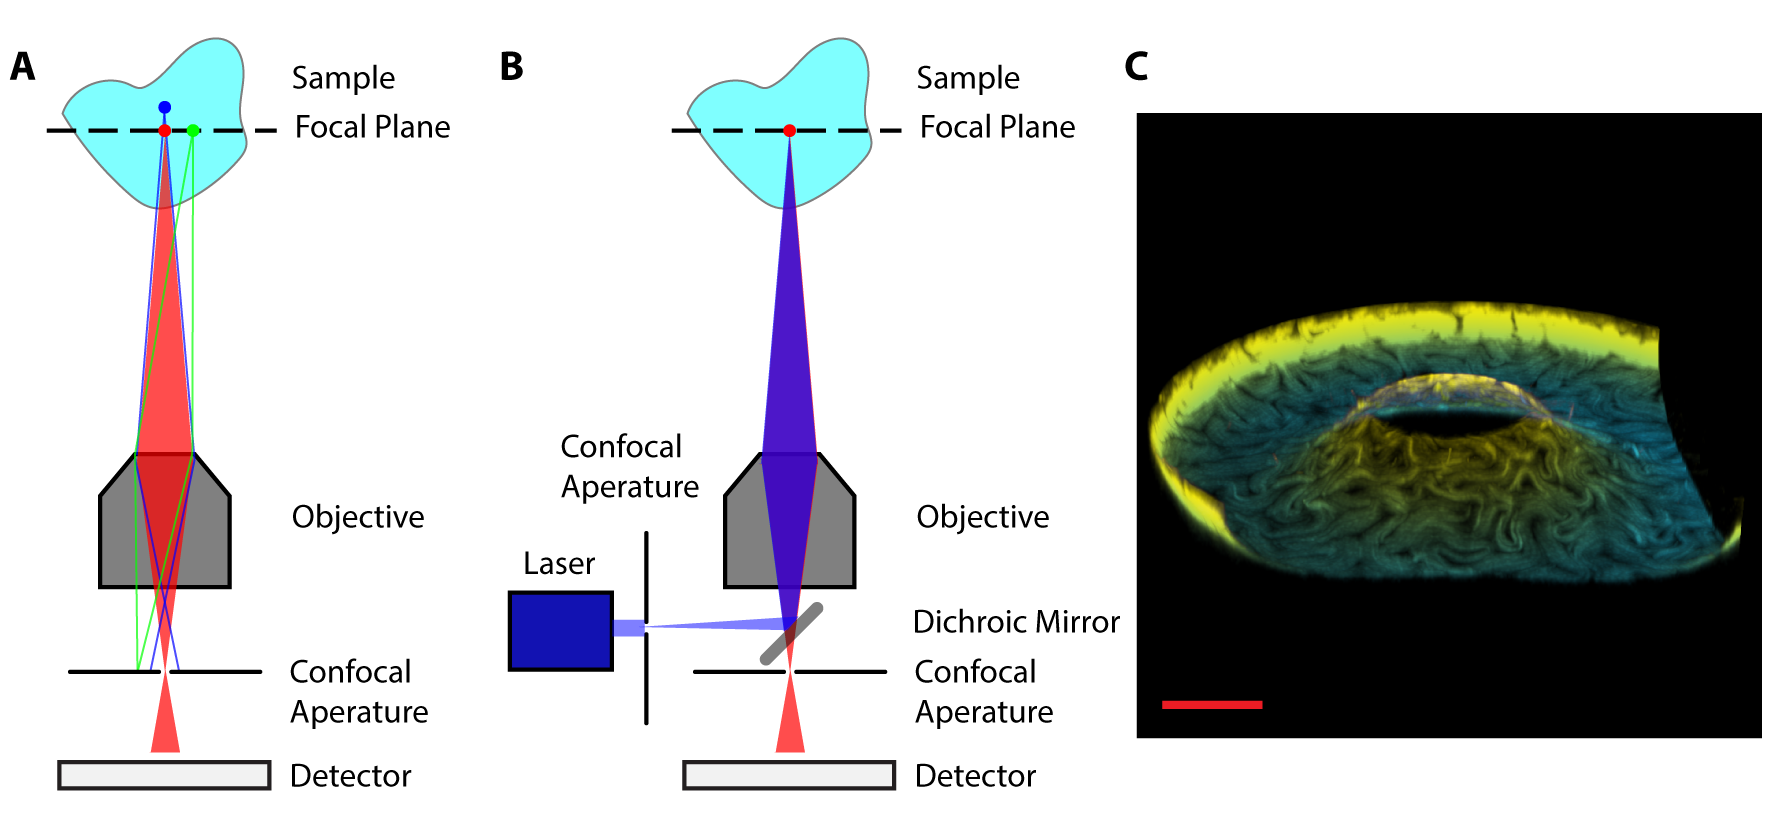
\includegraphics{figures/C3/Ch3-Figs_Confocal.png}
  \caption{Confocal microscopy.
  (A) Schematic showing the effect of the confocal aperture in front of the detector.
  Light from the red point is in focus at the aperture in the confocal plane, and thus can pass entirely through the aperture.
  In contrast, the blue light is emitted above the focal plane; the light is out of focus at the confocal plane and does not pass through the aperture.
  Similarly, the green light is in focus at the confocal plane, but it is not emitted from a conjugate point to the aperture and thus does not pass through the aperture.
  (B), Schematic of laser confocal fluorescence microscopy.
  There is a confocal aperture in front of the laser such that the laser is focused by the objective onto the focal plane in the sample.
  Thus, the maximum excitation will be at the conjugate point in the focal plane.
  As in (A), only the emitted light from the conjugate point in the focal plane is incident on the detector.
  A dichroic mirror allows the excited and emitted light to share the same path to and from the sample, but passes only the emitted light to the detector.
  Scanning mirrors (not drawn) between the dichroic mirror and the objective raster the conjugate point over the focal plane to construct a full image of the focal plane.
  (C) An example image stack of an active nematic torus, where the image stack has been reoriented to provide perspective and the data have been false-colored by height.
  This image stack was taken with a typical set of parameters: total size, 1.28~mm $\times$ 1.28~mm $\times$ 0.21~mm, pixel size, 2.5~$\upmu$m/px $\times$ 2.5~$\upmu$m/px $\times$ 7~$\upmu$m/px.
  The scale bar is 250 $\upmu$m.}\label{f:3-Confocal}
\end{figure}

\subsection{Confocal setup and parameters}
We used two different confocal microscopes to collect the data; we started with a Zeiss LSM 700 and then switched to a newer Nikon A1R when the latter was purchased by Professor Peter Yunker in the School of Physics.
Both instruments are scanning laser confocal microscopes.
Procedurally, both microscopes scan the image plane with a focused laser beam while recording the output intensity, adjust the height of the stage to change the focal plane, and then repeat the process until the image stack is acquired.
While the image stack can be thought of in terms of 3D voxels, the $z$-resolution between focal planes is less than the $xy$-resolution in the focal plane such that it is more convenient to think of the image acquisition as a stack of 2D images.

We note that we are inherently restricted to only imaging the lower half of the toroidal droplet due to refraction effects.
The light emitted from the upper half of the toroidal droplet travels through the aqueous active solution and then is refracted by the curved interface between the active solution and the yield stress material.
In contrast, the light from the lower portion of the toroid is emitted directly into the yield stress material such that its light path is unaffected by refraction.
However, even though we can in principle image up to the midpoint of the torus, in practice we typically stop our image stack below the midpoint.
This is because the time required to adjust the stage height is the slowest portion of the imaging process for both of the confocal microscopes we use.
Since we wish to acquire as many frames as possible for each toroid, we must balance the time required to take an image stack versus the size of the image stack.

The microtubules are dyed with AlexaFluor 647, which has an excitation peak at 651~nm and an emission peak at 667~nm~\cite{RN264}, as displayed in Figure~\ref{f:3-Spectra}(A).
Thus, we use a 633~nm laser as our illumination source and a Cy5 filter set such that only the emitted light reaches the detector.
The Cy5 filter set includes a 590~--~650~nm bandpass excitation filter, a 660~nm longpass dichroic mirror, and a 663~--~738~nm emission filter~\cite{RN263}.
The filters and mirror are designed with steep passband transitions such that the quoted ranges are good representations of the passband.
Note that for illumination with a laser, the excitation filter is unnecessary, but is standard when purchasing the filterset.
The excitation filter is necessary in wide-field fluorescence microscopy when illuminating with a white-light source.
\begin{figure}
  \centering
  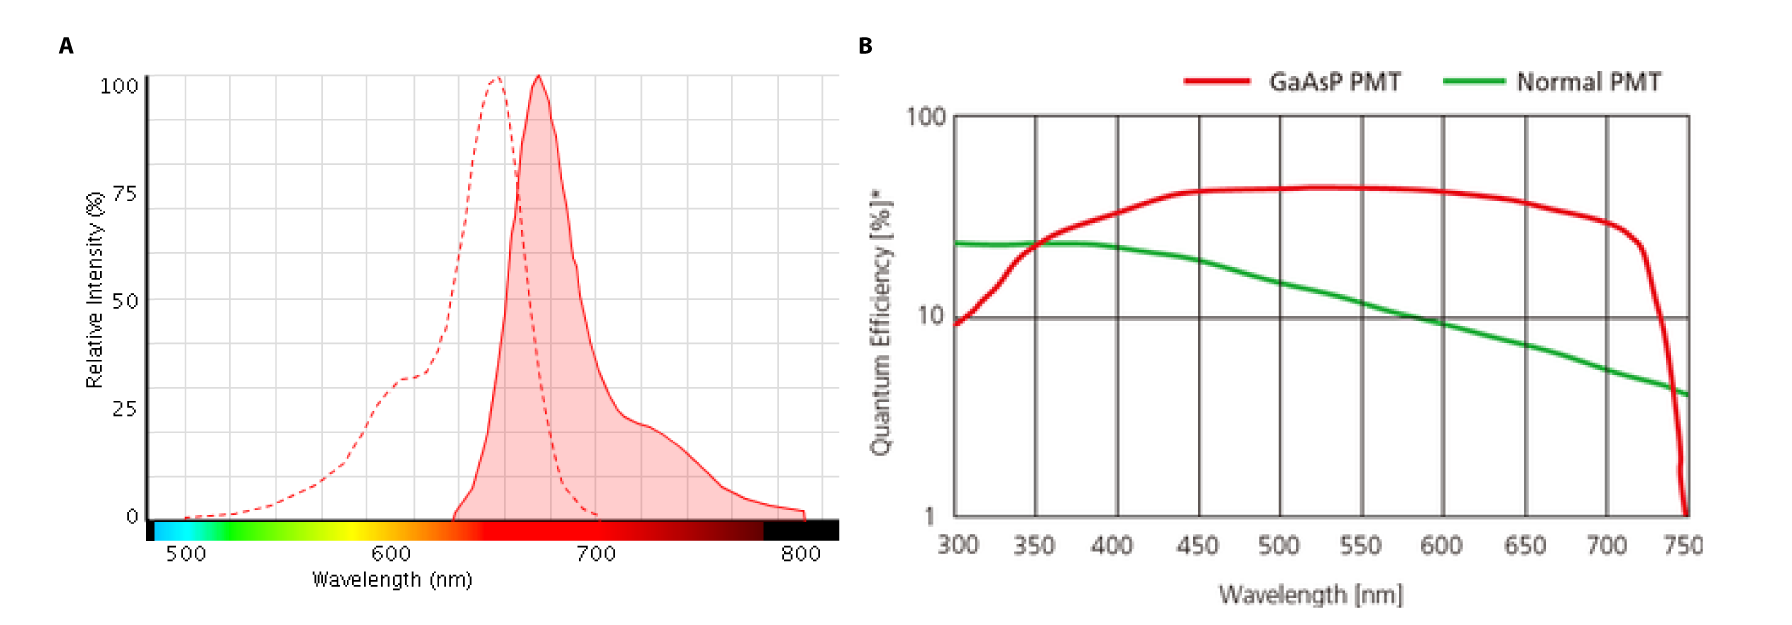
\includegraphics{figures/C3/Ch3-Figs_Spectra.png}
  \caption{Fluorophore spectra and detector quantum efficiencies for our experimental system.
  (A), AlexaFluor 647 (red dashed line) excitation and (shaded red area) emission spectra.
  Spectra from Ref.~\cite{RN264}.
  (B), Quantum effieciency as a function of wavelength for a (green line) standard PMT and a (red line) GaAsP PMT as a function of wavelength.
  Plot from Ref.~\cite{RN263}.}\label{f:3-Spectra}
\end{figure}

While the two confocal microscopes we used operate in the same manner, there are key differences that affect the quality of the data and thus affect the measurement protocol.
The Zeiss microscope uses standard photomultiplier tubes (PMT) as the detector.
Unfortunately, standard PMTs do not detect wavelengths above 600~nm well, as the quantum efficiency of the detector decreases with increasing wavelength and is typically below 10\% above that wavelength [green line, Figure~\ref{f:3-Spectra}(B)]~\cite{RN263}.
This means that we have to increase the intensity of the laser, increase the gain on the detector, and even average two scans of each image plane in order to increase the signal-to-noise ratio to an acceptable level.
As a result, data from the Zeiss microscope take longer to collect and the active nematic exhibits mild photobleaching for long acquisitions.
However, we note that the photobleaching is mild and does not decrease the signal-to-noise ratio enough to affect our data analysis.

In contrast, the Nikon microscope uses a Gallium Arsenide Phosphide (GaAsP) PMT in conjunction with standard PMTs to increase the quantum efficiency of the detector suite for larger wavelengths.
GaAsP PMTs maintain a roughly constant quantum efficiency of $\approx 50$\% up to 700~nm [red line, Figure~\ref{f:3-Spectra}(B)]~\cite{RN263}.
Thus, we can keep both the laser power and detector gain low while still only needing a single scan of the image plane to acquire a higher quality image stack than we get from the Zeiss microscope.
We therefore can acquire image stacks with a higher time resolution, a higher image quality, and with no noticeable photobleaching when using the Nikon microscope.

We set up a measurement as follows.
First, we place the sample on the microscope stage and find the toroidal droplet using standard brightfield microscopy.
We then select the 633~nm laser and Cy5 filter set from the available options on the microscope.
Next, we set the microscopes to scan the focal plane and display the output in real time.
We lower the stage to find the bottom of the sample, set this height to be the bottom of the image stack, and then raise the stage to determine the highest plane that we will measure.
As a rule of thumb we aim for 15~--~30 image planes, depending on the microscope used to acquire the data.
If we image too few planes, we don't image the highly curved areas of the droplet.
If we image too many planes, we don't acquire enough frames over the life of the active nematic.
Each 512 px $\times$ 512 px image plane typically takes 0.8~s to acquire, and it takes about 1~s to move between planes.
Overall, this means that a full image stack takes between 30~s and 1~min to acquire.

Now that we have set up the size of the image stack, we turn to adjusting the laser intensity and gain to produce the highest quality images.
The laser intensity incident on the sample is tuned by an acousto-optical tunable filter (AOTF) placed at the output of the laser, and before the laser enters the confocal microscope.
An AOTF is a tunable diffraction grating, where the grating is formed by standing acoustic waves that create a periodic index of refraction.
By changing the frequency of the acoustic waves, the AOTF will diffract more or less light into the confocal microscope~\cite{RN317}.
The gain in the detector corresponds to the voltage applied across the dynodes in the photomultiplier tubes~\cite{RN316}.
This is controlled in the imaging software by a slider from 1 to 255, with 1 corresponding to the minimum operating voltage and 255 the maximum operating voltage.
We first find the image plane with the brightest intensity, and manipulate the intensity and gain such that at most $\approx 5$\% of the pixels are saturated.
While a higher laser power and lower gain will produce better quality images, setting the laser power too high can lead to excessive photobleaching for long time measurements.
We typically set the laser power to approximately 3\% of the maximum 15 mW output.
With this laser power, we need a gain roughly halfway between the minimum and maximum values.
If we are on the Zeiss microscope, we set the microscope to scan each image plane twice and average the measurements such that we can reduce the overall laser power and minimize photobleaching.

For both microscopes, we then go to the bottom plane where the emitted intensity is weakest and set an offset corresponding to an intensity floor for the measurement.
Pixels with an intensity below the offset are set to 0.
This helps to remove some of the thermal noise in the image; in practice, we have enough signal that this parameter does not really matter.

Once these parameters have been set, we turn on a focusing system to eliminate the effect of thermal and mechanical drift in the measuring system.
Ambient temperature changes and mechanical slop in the measuring system cause the measured distance between the objective and a given reference plane in the sample to change over time.
This will result in the physical sample volume imaged by the confocal changing over time.
The focusing system uses a lens and an LED to form an image of the interface between the coverslip or microscope slide and the sample.
Turning on the focusing system corresponds to the software adjusting the lens to form the image of this interface without changing the current height of the microscope stage.
The software then maintains this image of the interface by adjusting the height of the microscope stage, naturally compensating for thermal drift and mechanical slop.
By maintaining this image of the interface, the focusing system naturally maintains the focal plane of the confocal microscope in the sample.

Finally, we set the microscope to image continuously for 12 hours, starting the next image stack as soon as it finishes the previous stack until the 12 hours have expired.
We note that files imaged for longer than 12 hours can be difficult to work with due to their large size.
Once the image acquisition is finished, we crop the raw confocal time series to only include the portion where the toroidal droplet is active.
We save this cropped version in single multi-page \texttt{.tiff} file including the metadata containing acquisition parameters.
This standardizes the data format between the different microscopes to make it easier to read in to the computer.


\subsection{Inputting confocal data into MATLAB}
The core routine to load the image stack into MATLAB comes from the \texttt{bioformats} toolbox put out by the Open Microscopy Environment~\cite{RN265}.
The Open Microscopy Environment maintains the open-source \texttt{OME-TIFF} image format for microscopy data.
The \texttt{bioformats} toolbox allows us to call the imaging parameters such as pixel-to-length conversions, framerate, etc., as well as access the total times series of image stacks as a 3D array in MATLAB.
The data are stored as a stack of 2D arrays, where each array holds data from a measurement of a confocal plane at a moment in time.
The 2D arrays are stored in the order that they were taken; this corresponds to concatenating the full 3D image stacks along the $z$ direction in the order the individual stacks were taken.
Thus, to locate a specific 3D image stack you have to know which stack in the time series you want as well as the number of planes in each image stack.
Since the entire image series from the confocal can be up to 8~Gb, we first extract the relevant data and then remove the image series from memory so that we have the free memory needed to analyze the data.

We first determine the surface of the toroidal droplet by averaging the image planes at a given height over time and then applying an intensity threshold.
Since we have fluorescence confocal data where the fluorescent media has depleted to the surface of the torus, averaging over time creates a clear intensity image of the toroidal surface as both transient structures in the bulk as well as the filamentary structures of the active nematic are washed out in the averaging process, as seen in the example images in Figure~\ref{f:3-SurfaceHeight}(A,B).
We next threshold the data to binarize the image stack; this lets us make the distinction between the surface of the toroidal droplet and everything else.
There are a large range of threshold values that do not change the shape of the surface or affect the final curvature values; we choose the smallest threshold value that produces a smooth surface with no extraneous bright pixels that are not on the surface.

From the binarized 3D array, we look at every $xy$ position and determine the lowest $z$ value that contains a nonzero value.
We take this $z$ value to be the height $h$ of the toroidal surface and record it in an array, giving us $h = f(x,y)$, as shown in Figure~\ref{f:3-SurfaceHeight}(C) for the example image in Figure~\ref{f:3-SurfaceHeight}(B).
This is commonly known as a Monge parameterization of the surface~\cite{RN23}.
\begin{figure}
  \centering
  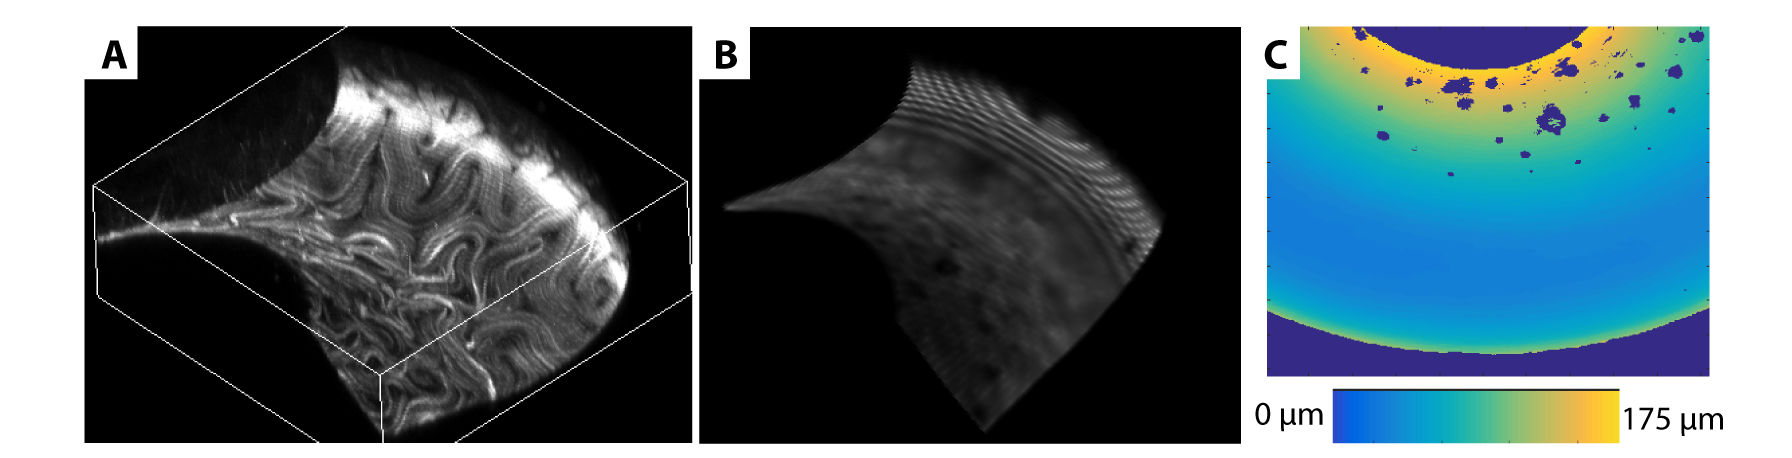
\includegraphics{figures/C3/Ch3-Figs_SurfaceHeight.png}
  \caption{Determining the surface of a toroid from confocal microscopy data.
  (A) Example confocal image stack at a moment in time.
  (B) The average over time of all the image stacks.
  Here, the averaging washes out stray filaments in the bulk as well as the nematic structure of the filaments, as seen in (A), giving us an intensity image of the surface itself.
  (C) The height of the surface $h(x,y)$, where $h$ is determined by thresholding (B) and then averaging the height of the bright pixels in the thresholded image stack for every $(x,y)$ position.}\label{f:3-SurfaceHeight}
\end{figure}

We next consider the intensity stack for each time point and perform a maximum intensity projection into the $xy$-plane with the caveat that we only consider pixels that are within $\pm 5$ z-stack planes of the height at each individual point.
This process largely prevents transient bright filaments in the bulk of the toroidal droplet from affecting our measurements.
Thus, we now have recorded our surface and reduced our data from a time-series of 3D image stacks to a time-series of 2D images such that we have the intensity $I = f(x,y,t)$.
An example projection at an instant in time for the image stack in Figure~\ref{f:3-SurfaceHeight}(A) is shown in Figure~\ref{f:3-CEDF2}(A).
Once we have extracted the time-series of data on the surface, we work to: (i) determine the director and defects from the intensity projections, and (ii) calculate the surface curvature and surface normals using $h(x,y$).




\section{Determining director and defects}
In the intensity projection of a confocal stack at a time $t_0$, $\mathbf{n}$ is given by the direction of the microtubule bundles.
This direction is obtained from the grayscale image by finding the direction along which the intensity fluctuates the least for each pixel using a technique called coherence-enhanced diffusion filtering (CEDF)~\cite{RN30}.
CEDF is used extensively in computer vision and in cell segmentation in biology, but it has not yet been used in the Physics literature~\cite{RN137}.
We illustrate this technique with an example analysis of the intensity projection shown in Figure~\ref{f:3-CEDF2}(A).


\subsection{Coherence-enhanced diffusion filtering}
To begin with, the original intensity image $I = I(x,y,t_0)$ is denoised using a Gaussian blur of standard deviation $\sigma$ and side length $6 \sigma -1$ to lessen contributions to the intensity fluctuations from random noise, giving us the blurred image $I_{\sigma}$.
The result of blurring the example image as well as the inset isolated defect pair in Figure~\ref{f:3-CEDF2}(A) is seen in the main image and inset of Figure~\ref{f:3-CEDF2}(B), respectively.
This blur was performed using a $5 \textrm{ px} \times 5 \textrm{ px}$ Gaussian filter with $\sigma= 1$ px.

Next, the gradient tensor for $I_{\sigma}$ is calculated for each pixel:
\begin{equation}
(\nabla I_{\sigma})(\nabla I_{\sigma})^T =
\begin{bmatrix}
(\nabla_x I_{\sigma})(\nabla_x I_{\sigma}) & (\nabla_x I_{\sigma})(\nabla_y I_{\sigma}) \\
(\nabla_y I_{\sigma})(\nabla_x I_{\sigma}) & (\nabla_y I_{\sigma})(\nabla_y I_{\sigma})
\end{bmatrix}.
\end{equation}
Since the microtubule bundles have head-tail symmetry, we cannot use the gradient vector alone to define the bundle orientation as the vector has a defined head and tail.
The rank-2 gradient tensor is symmetric and is the same whether it is constructed with the gradient vector or the negative gradient vector.
Thus, we use the gradient tensor to ``remove the head'' from the gradient vector.

We now define the coherence direction of a symmetric rank-2 tensor as the direction of the eigenvector associated with the smallest eigenvalue.
Recall that according to the Spectral theorem, any symmetric real matrix is diagonalizible, with the diagonal elements the eigenvalues of the matrix and the associated orthonormal basis formed by the eigenvectors.
The coherence direction represents the direction along which the spatial intensity fluctuations are the weakest and is defined on the interval $[0^{\circ}, 180^{\circ})$.
The coherence direction calculated for the gradient tensor of each pixel for $I_\sigma$ shown in the main image and inset of Figure~\ref{f:3-CEDF2}(B) is seen in the main image and inset of Figure~\ref{f:3-CEDF2}(C), where the orientation of the coherence direction on the interval $[0^{\circ}, 180^{\circ})$ measured clockwise (CW) off of the horizontal axis has been mapped to the grayscale intensity values $[0,255)$, with 0 corresponding to black and 255 to white.
We see that there are still too many fluctuations in the coherence directions shown in Figure~\ref{f:3-CEDF2}(C) to determine $\mathbf{n}$.

We remove the remaining small-scale fluctuations in this image by performing another average, this time a component-wise average of the gradient tensor for each pixel.
This operation gives us the structure tensor for each pixel and can be written as:
\begin{equation}
K_{\rho} \ast (\nabla I_{\sigma})(\nabla I_{\sigma})^T =
\begin{bmatrix}
K_{\rho} \ast ( \nabla_x I_{\sigma})(\nabla_x I_{\sigma}) & K_{\rho} \ast (\nabla_x I_{\sigma})(\nabla_y I_{\sigma}) \\
K_{\rho} \ast (  \nabla_y I_{\sigma})(\nabla_x I_{\sigma}) & K_{\rho} \ast (\nabla_y I_{\sigma})(\nabla_y I_{\sigma})
\end{bmatrix},
\end{equation}
where $K_{\rho}$ is a Gaussian filter with standard deviation $\rho$, where $\rho$ should be about the size of the relevant coherence feature in the image, and $\ast$ is a convolution.
If $\rho$ is too small, the coherence directions of the structure tensor will resemble those from the gradient tensor, while if $\rho$ is too large the desired coherence features will be washed out by the averaging.

The coherence direction of the structure tensor calculated with $\rho = 5$ px and filter size $29\textrm{ px } \times 29$ px for each pixel of $I_{\sigma}$ seen in the main image and inset of Figure~\ref{f:3-CEDF2}(B), is shown in the main image and inset in Figure~\ref{f:3-CEDF2}(D), respectively.
As before, the orientation on the interval $[0^{\circ}, 180^{\circ})$ measured CW off of the horizontal axis has been mapped to the grayscale intensity values $[0,255)$.
 We note that the coherence direction of the structure tensor for each pixel represents the local director and corresponds to the ``molecular director,'' $\mathbf{u}$.
\newpage
\begin{figure}[H]
  \centering
  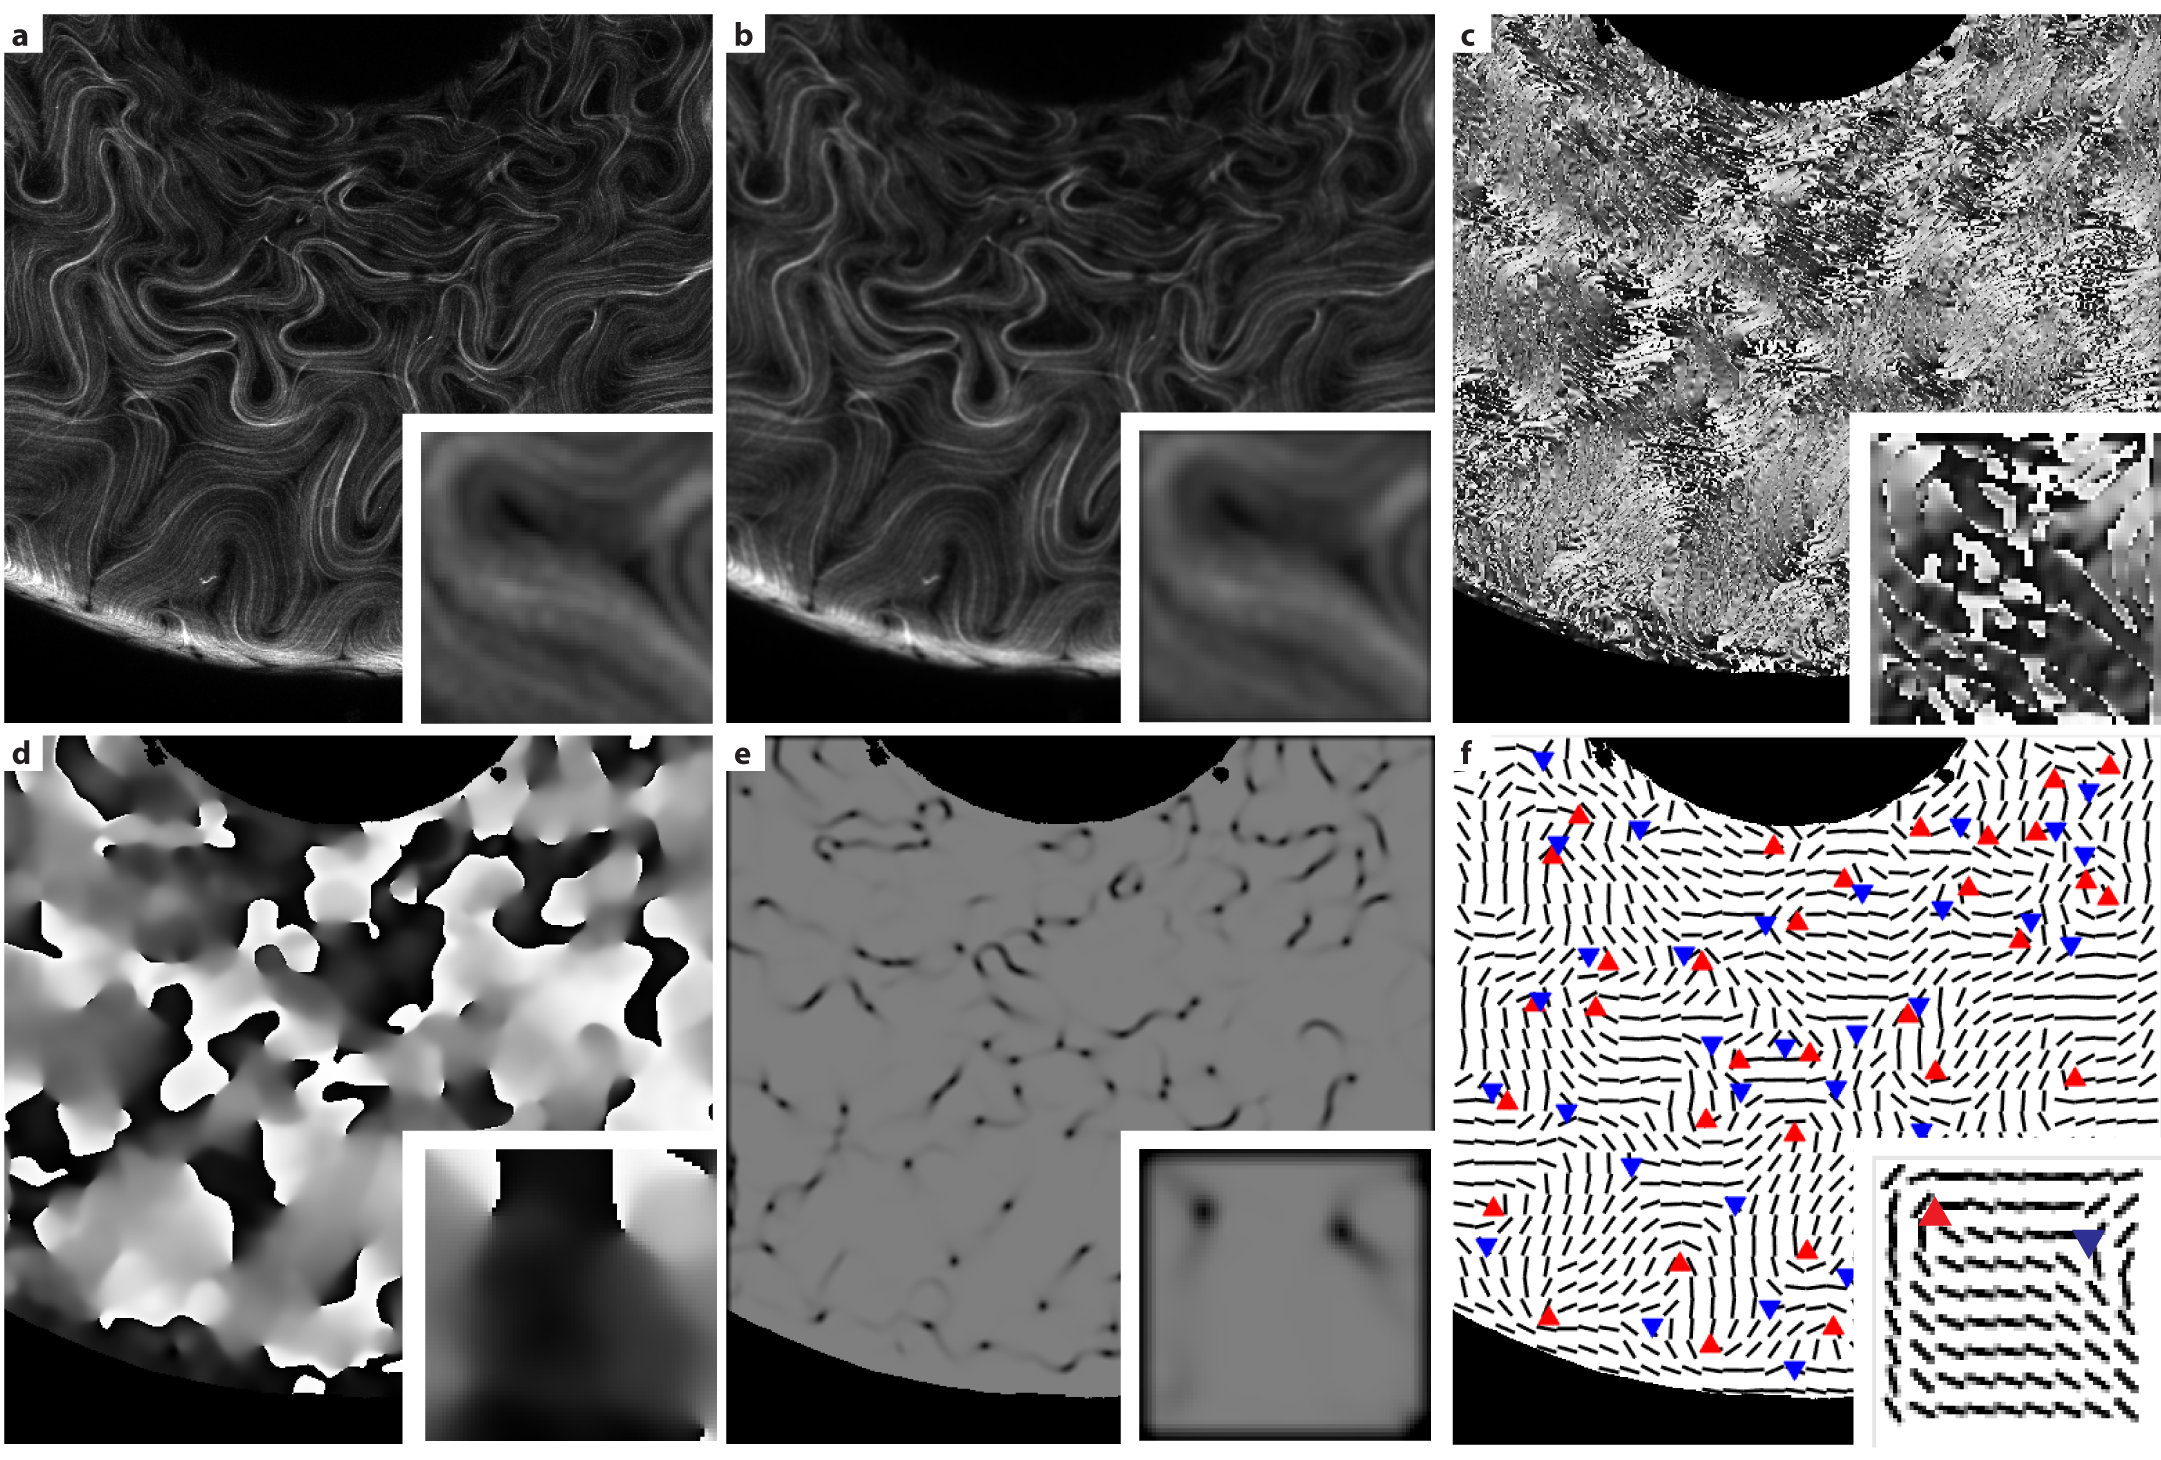
\includegraphics{figures/C3/Ch3-Figs_CEDF2.png}
  \caption{Step-by-step output to find the director and defects from an active nematic image.
(A), Maximum-intensity projection of a confocal stack onto the $xy$ plane for a single frame.
Inset: Close up of a defect pair.
(B), Image from (A) after applying a 5~px~$\times$~5~px Gaussian blur with standard deviation 1~px.
Inset: The same operation applied to the image in the inset of (A).
(C), Coherence directions of the tensors formed from the gradient of the image in (B).
Black represents $0^{\circ}$ and white represents $180^{\circ}$ measured CW from the horizontal.
Inset: The same operation applied to the image in the inset of (B).
(D), Coherence directions of the structure tensors formed by component-wise averaging the gradient tensors formed from image (B).
Black represents $0^{\circ}$ and white represents $180^{\circ}$ measured CW from the horizontal.
The averaging is done with a 29~px~$\times$~29~px Gaussian filter with standard deviation 5~px.
Inset: The same operation applied to the image in the inset of (B).
(E), The scalar order parameter $S$ obtained by diagonalizing the $\mathbf{Q}$ formed from the directions in image (D).
$\mathbf{Q}$ is formed for each point by considering the directions of all points in a 5 pixel radius.
Inset: The same operation applied to the image in the inset of (D).
(F), The director obtained by diagonalizing the $\mathbf{Q}$ formed from the direcions in image (D).
$\mathbf{Q}$ is formed for each point by considering the directions of all points in a 5 pixel radius.
The defects are calculated by considering points of low $S$ and calculating the $\mathbf{n}$-rotation along a path encircling the point.
$s = +1/2$ defects are represented by ${\color{red} \blacktriangle  } $  and $s = -1/2$ defects are represented by ${ \color{blue} \blacktriangledown  } $.
Inset: The same operation applied to the image in the inset of (D).}\label{f:3-CEDF2}
\end{figure}
\newpage
\subsection{Calculating the director}
From $\mathbf{u}$, we compute the 2D tensor nematic order parameter defined in Eq.~\ref{e:2-2DOrderRaw}, taking the average over the $\mathbf{u}$ of all points within a specified radius $\beta$ of the point of interest.
We perform this averaging using a mean filter of radius $\beta$.
We then diagonalize $\mathbf{Q}$ as shown in Eq.~\ref{e:2-2DOrderDiag}, providing $\mathbf{n}$ and $S$ for each pixel.
For the orientations of $\mathbf{u}$ that are displayed in Figure~\ref{f:3-CEDF2}(D), we choose $\beta = 5$~px to produce $S$ and $n$ as shown in Figure~\ref{f:3-CEDF2}(E,F), respectively.
We map the values $S = [0, 1]$ in Figure~\ref{f:3-CEDF2}(E) to the grayscale intensity values $[0,127]$ such that black represents $S = 0$ and the lightest gray represents $S = 1$.
Thus, the dominant gray shade in Figure~\ref{f:3-CEDF2}(E) indicates uniform alignment within the 5 px radius.
We chose this map so that we can display $S$ on top of either a white background or a black background.
In addition, note that only every $7^{\textrm{th}}$ value of $\mathbf{n}$ is plotted in Figure~\ref{f:3-CEDF2}(F) to ensure the $\mathbf{n}$-field is clear to the eye.
In reality there is a value for $\mathbf{n}$ at every pixel.

The process of determining the director relies on the choice of three parameters: $\sigma$, the standard deviation of the filter for the initial blur, $\rho$, the standard deviation of the filter to produce the structure tensor, and $\beta$, the radius of the disc filter used to determine $\mathbf{Q}$.
We choose the parameters such that the director field calculated on a random sampling of 3~--~5 intensity images in a given time series best agrees by eye with the actual intensity images.
We find best results keeping $\sigma = 0.5$~px and varying $\rho$ between 5~px and 8~px and varying $\beta$ between 5~px and 6~px.
The variations in $\rho$ and $\beta$ are a result of different scales between pixels and $\upmu$m depending on the microscope used, the microscope zoom, and the output image size.
However, since the initial blur is responsible for removing random noise at the pixel level, we find best results keeping $\sigma = 0.5$ px always.
Once we determine $\mathbf{n}$ and $S$, we are ready to find the defects.


\subsection{Finding defect location and topological charge}
We mentioned in Chapter~\ref{c:1} that defects are singularities in the director field; in addition, $S \ll 1$ at a defect.
Therefore, we start by selecting pixels with $S < 0.1$ as potential defect candidates.
For every candidate, we first consider all pixels in a 5~px~$\times$~5~px plaquette centered on the point of interest and ensure that there are no other candidates in the plaquette with a lower value of $S$.
We then calculate the $\mathbf{n}$-rotation about the point of interest according to Eq.~\ref{eq:2-topCharge}.
Explicitly, we numerically evaluate $s = (1 / 2 \pi)\oint \frac{\partial\phi}{\partial u} \, \textrm{d}u$ counterclockwise (CCW) along the edge of the plaquette, where $u$ is the arclength along the square contour and $\phi$ is the orientation of $\mathbf{n}$.
We take the point of interest to be a $s = \pm 1/2$ defect if $s \in \pm [0.49,0.51]$.
The $s=\pm1/2$ defects calculated for our example analysis are plotted on top of the $\mathbf{n}$-field in Figure~\ref{f:3-CEDF2}(F), with $s = +1/2$ defects indicated by ${\color{red} \blacktriangle } $  and $s = -1/2$ defects indicated by ${ \color{blue} \blacktriangledown } $.

We store the defect locations in a list recording the frame and position of each defect.
The $s = +1/2$ and $s = -1/2$ defects are stored separately.
For toroids made with 36 $\upmu$M ATP, our time resolution is high enough to track the defects.
We track $s = +1/2$ and $s = -1/2$ defects independently using a combinatorics-based particle tracking algorithm~\cite{RN54,crockerGrierNotes}.
For tracked defects, we store the defect identity in addition to the frame and position so that we can reconstruct individual defect trajectories.


\subsection{Measuring defect charge in a specified region}
Once we have identified all the defects in every frame, we want to be able to look at a specific region on the torus and determine the topological charge in that region over time.
We do this by placing the defect locations at each time frame into a binary array, or mask, where a ``1'' indicates a defect and the rest of the array is set to ``0''.
We create separate arrays for the $s = + 1/2$ and $s = - 1/2$ defects.
We then concatenate the masks such that the final binary arrays $J^{(+)}(x,y,t)$ and $J^{(-)}(x,y,t)$ hold the $s = +1/2$ and $s = -1/2$ defects over time, respectively.
Now, if we have a binary mask defining a region $\Theta(x,y)$, where pixels in the region have a value of 1 and pixels outside of the region have a value of $0$, determining the number of $s = +1/2$ and $s = -1/2$ defects in a region over time, $N^{(\pm)}_{\Theta}(t)$, is a matter of calculating the sum $N^{(\pm)}_{\Theta}(t) = \sum\limits_{x,y}\,J^{(\pm)}(x,y,t)\Theta(x,y)$.
We plot $N^{(\pm)}_{\Theta}(t)$ and $N_{\Theta}(t) = N^{(+)}_{\Theta}(t) + N^{(-)}_{\Theta}(t)$ in the example region in Figure~\ref{f:3-NumberOverTime}(A) over time in Figure~\ref{f:3-NumberOverTime}(B), showing that both $N^{(\pm)}_{\Theta}(t)$ and $N_{\Theta}(t)$ fluctuate, with the fluctuations in each quantity centered around a mean.
Thus, given $\overbar{N}^{(\pm)}_{\Theta} = (1/T)\sum\limits_{t = 0}^T \, N^{(\pm)}_{\Theta}(t)$, the time-averaged number of $s = \pm 1/2$ defects over a time period $T$, we can calculate the time-averaged topological charge in a region as $\overbar{s}_{\Theta} = (\overbar{N}^{(+)}_{\Theta} - \overbar{N}^{(-)}_{\Theta})/2$.
\begin{figure}
  \centering
  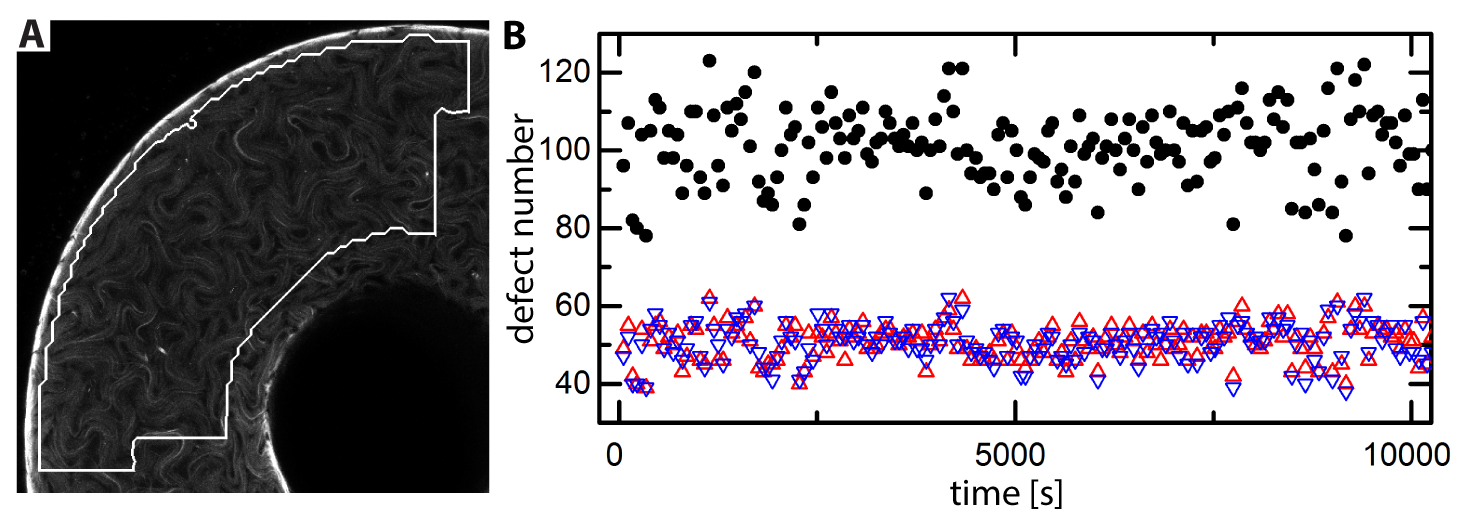
\includegraphics{figures/C3/Ch3-Figs_NumberOverTime.png}
  \caption{Defect number fluctuations in a region.
  (A) The region outlined in white has $(1/2\pi)\int K\, \textrm{d}A = 0$ and Area $A = 0.795$ mm$^{-2}$.
  (B) Plot of the number of $({\color{red} \vartriangle})$ $s = + 1/2$ defects, $({\color{blue} \triangledown})$ $s = -1/2$ defects, and $(\bullet)$ total number of defects over time in the region highlighted in (A).}\label{f:3-NumberOverTime}
\end{figure}

Due to the discrete nature of our data, it is possible to ``miss'' defects, especially when a pair of defects are close together.
Typically, since one defect in the pair will have a lower value of $S$, the defect with the larger value of $S$ will be ignored.
Since topological charge is a discrete quantity, every missed defect in a region causes the total topological charge in that region to have an error of $\pm 1/2$.
This gives us a way to characterize the error in our defect-finding routine.
If the error is completely random, the measured time-averaged topological charge, $\overbar{s}_{\Theta}$, will converge to the actual value of the time-averaged topological charge, $\overbar{s}_{\Theta}^{actual}$.
However, if there is a systematic error, $\overbar{s}_{\Theta}$ will converge to $\overbar{s}_{\Theta}^{actual} \pm n/2$, where $n \in \mathbb{N}$.
For example, if our routine were to always miss a single $s = +1/2$ defect, $\overbar{s}_{\Theta} - \overbar{s}_{\Theta}^{actual} = -1/2$.
We first monitor $\overbar{s}_{\Theta}$ as a function of averaging time to check for convergence, as shown for three regions in Figure~\ref{f:3-ChargeOverTime}.
We find that the time-averaged topological charge in a region converges if we average over enough time frames.
Next, we use topology to quantify the error in every measurement and rule out a systematic error in our analysis.
\begin{figure}
  \centering
  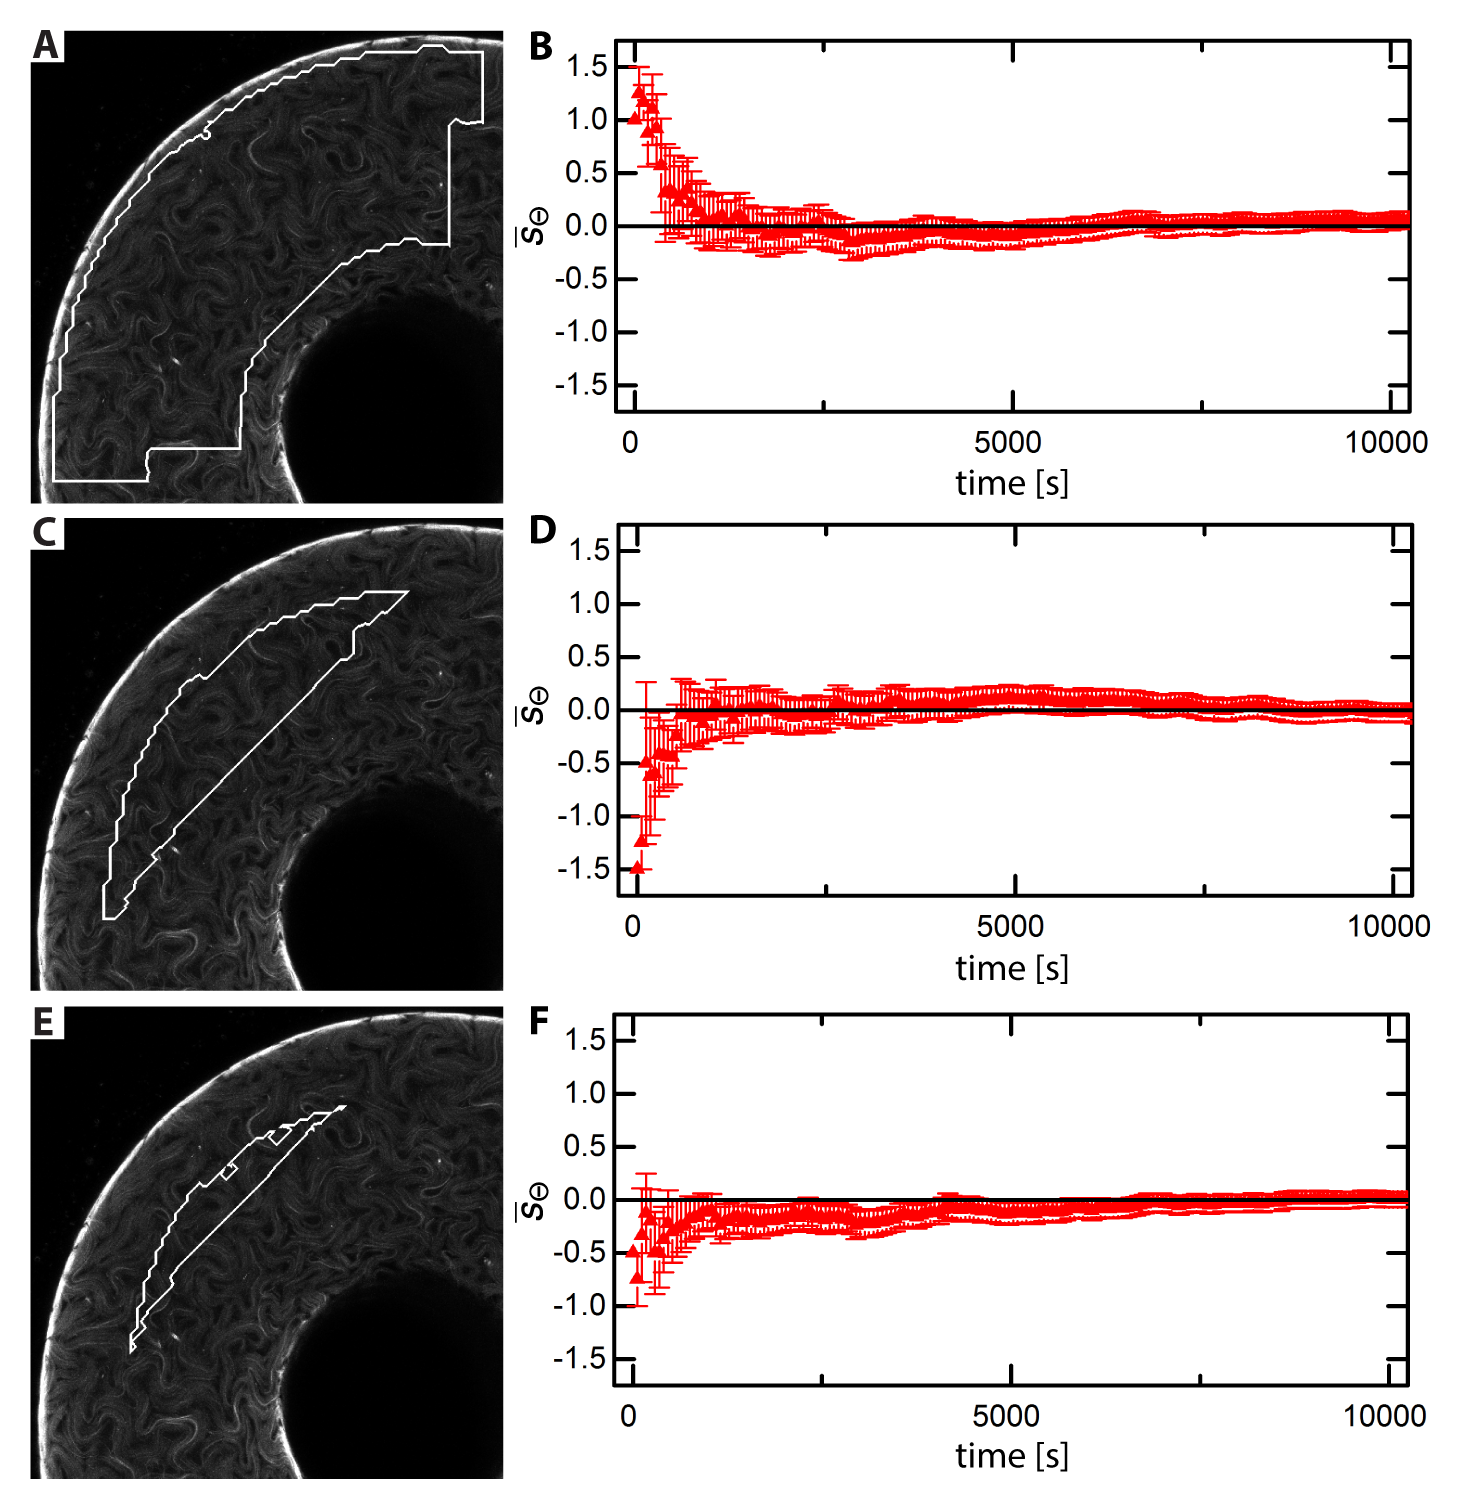
\includegraphics{figures/C3/Ch3-Figs_ChargeOverTime.png}
  \caption{Time-averaged topological charge measured for different areas on a toroid with $\xi = 2.0$ and $a = 372$ $\upmu$m.
  (A,C,E) The region outlined in white has (A) $(1/2 \pi) \int K \, \textrm{d}A = 0$ and area $A = 0.795$ mm$^{-2}$, (C) $(1/2 \pi) \int K \, \textrm{d}A = 0$ and area $A = 0.211$ mm$^{-2}$, (E) $(1/2 \pi) \int K \, \textrm{d}A = 0$ and area $A = 0.064$ mm$^{-2}$.
  (B,D,F) Plot of time-averaged topological charge vs averaging time for the region highlighted in (A,C,E), respectively.
  The error for each point is the standard error of the mean.
  }\label{f:3-ChargeOverTime}
\end{figure}

We test for a systematic error in the measured topological charge by considering a region of interrogation as its own entity, i.e. a compact surface with a boundary.
Note that a compact surface with a boundary is topologically like a disc.
For a compact surface with a boundary, we can write the Gauss-Bonnet theorem as:
\begin{equation}
  \chi = 2(1-g)-h,\label{e:3-GB3}
\end{equation}
where $\chi$ is the Euler characteristic, $g$ is the genus, and $h$ is the number of boundaries.
Thus according to Eq.~\ref{e:3-GB3}, our regions of interrogation have $\chi = 1$.
Importantly, the Poincar\'e-Hopf theorem as written in Eq.~\ref{e:1-PH} only applies for surfaces with a boundary if the director at the boundary is either everywhere tangential or everywhere normal to the boundary.
In our case, the director is free to take any value on the boundary and thus can act as a source or sink of topological charge such that we can't write a relation between only the topological charge on the surface and the Euler characteristic of the surface.

Instead, we must use an extended version of the Poincar\'e-Hopf theorem~\cite{RN267} that accounts for variations of the director on the boundary:
\begin{equation}
  \chi = s_{bulk} + s_{boundary} = \sum\limits_i s_i + s_{boundary},\label{e:3-extendedPH}
\end{equation}
where $s_i$ is the charge of a defect in the bulk of the region calculated via Eq.~\ref{eq:2-topCharge}, and $s_{boundary}$ is called the edge or boundary charge.


\subsection{Edge charge}
Recall that the topological charge is the winding number of the director along a closed contour in real space, where the director is specified with respect to a fixed frame.
To find the edge charge we consider $\mathbf{n}$ along the edge and calculate the associated winding number in $\mathbb{R}\mathbb{P}_1$, but here we measure the director orientation with respect to a moving frame on the boundary.
This moving frame is called the Frenet-Serret frame and is defined by the unit tangent vector, $\mathbf{T}$, and unit normal vector, $\mathbf{k}$, along the boundary.
If we let $\phi$ describe the director orientation with respect to the fixed coordinate system and $\psi$ describe the orientation of $\mathbf{T}$ with respect to the fixed coordinate system, then $\phi' = \psi-\phi$ gives the director orientation with respect to the Frenet-Serret frame~\cite{RN35,RN23}.
These two frames and the associated angles are illustrated in Figure~\ref{f:3-EdgeChargeEx}(A).
Thus, we calculate the edge charge like:
\begin{equation}
  s_{boundary} = \frac{1}{2\pi} \oint \textup{d}\phi'\label{e:3-boundCharge}.
\end{equation}
As a check, we can substitute the definition of $\phi'$ into Eq.~\ref{e:3-boundCharge} and re-write the edge charge as:
\begin{equation}
  s_{boundary} = \frac{1}{2\pi} \oint \bigg \{ \textup{d}\psi - \textup{d}\phi \bigg \} = \frac{1}{2\pi} \oint \textup{d}\psi - s_{bulk}.\label{e:3-boundChargeExpand}
\end{equation}
If we perform the integral in Eq.~\ref{e:3-boundChargeExpand} in the direction of the unit tangent vector, the Turning of Tangents theorem says that $ \oint \textup{d}\psi = 2\pi$~\cite{RN35}.
Thus, $s_{boundary} = 1 - s_{bulk}$ such that we recover $\chi = s_{bulk} + s_{boundary} = 1$, as required for our surface with a single boundary.

For example, consider a uniform director filed in a circular region, as drawn in the upper part of Figure~\ref{f:3-EdgeChargeEx}(B).
There is no defect in the bulk, so $s_{bulk} = 0$.
Now considering the director variation along the boundary in the Frenet-Serret frame, as drawn in the lower part of Figure~\ref{f:3-EdgeChargeEx}(B), we see that the director rotates by $2 \pi$, corresponding to $s_{boundary} = 1$ and thus $s_{bulk} + s_{boundary} = 1$.
This is illustrated in Figure~\ref{f:3-EdgeChargeEx}(C,D) with further examples where the circular region contains a director field with a single $s = +1$ defect, and where the director field has a single $s=-1/2$ defect, respectively.

We can determine if we have systematic error in our defect detection routine with Eq.~\ref{e:3-extendedPH}, as the sum of the edge charge and the topological charge from all the defects in the bulk should be equal to 1.
We do this by independently determining $s_{boundary}$ using Eq.~\ref{e:3-boundCharge} and $s_{bulk}$ using our defect-finding algorithm.
\begin{figure}
  \centering
  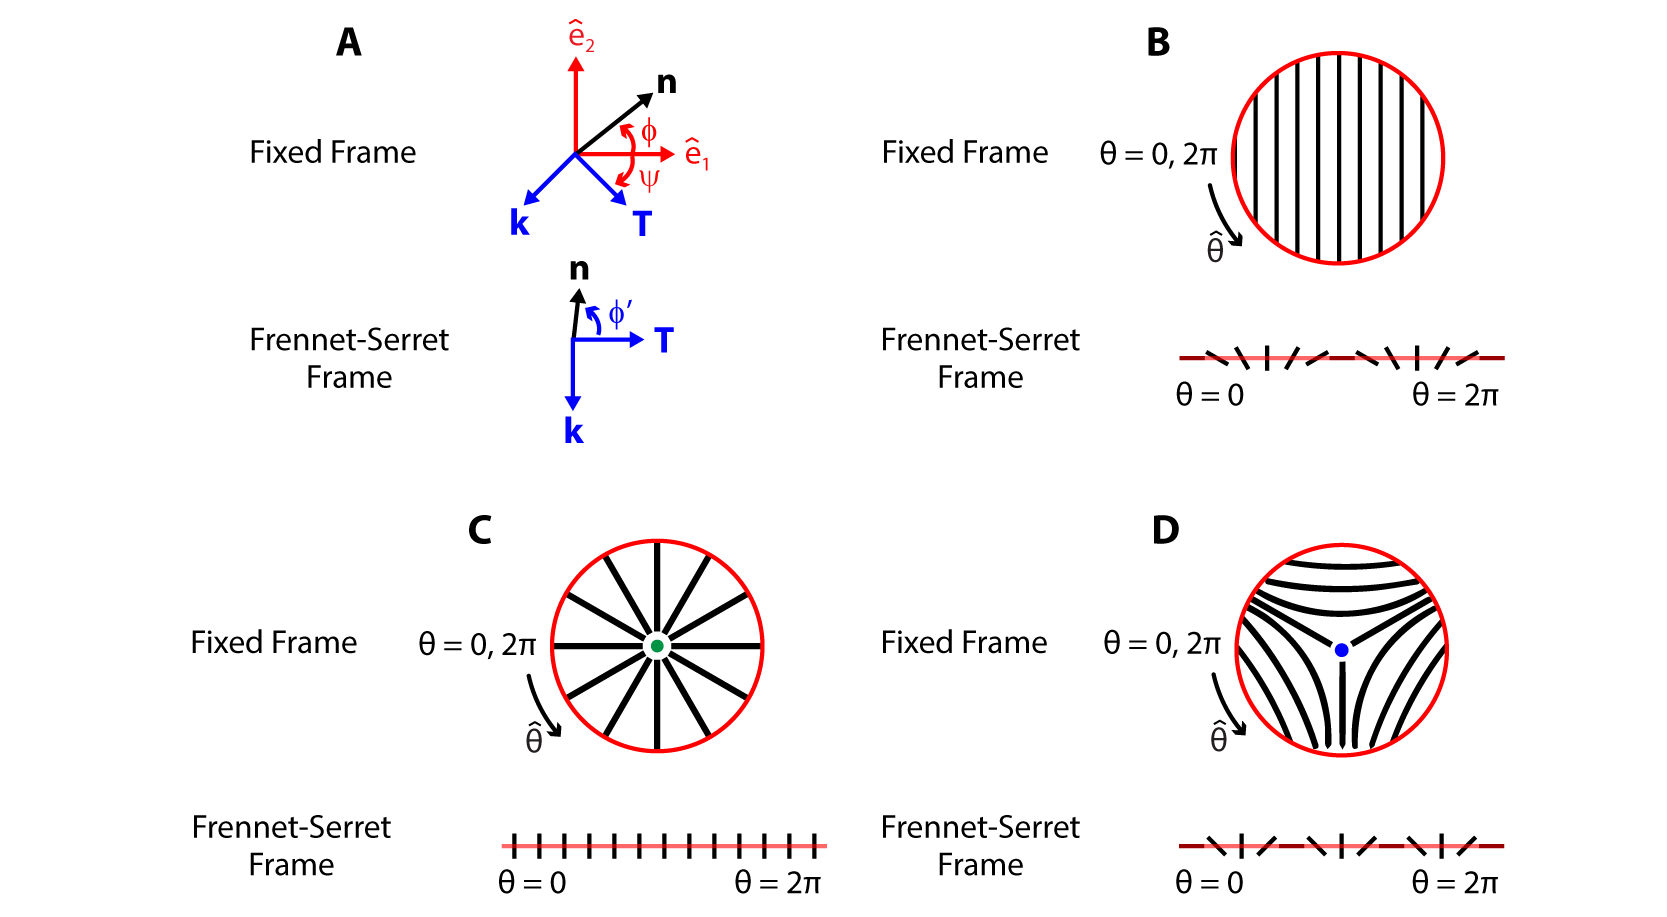
\includegraphics{figures/C3/Ch3-Figs_EdgeChargeEx.png}
  \caption{Schematic illustration of boundary and bulk charge.
  (A), The fixed frame is defined by the orthonormal basis $\{\hat{e}_1, \hat{e}_2 \}$.
  The Frenet-Serret frame is a moving orthonormal frame defined by the unit tangent vector and unit normal vector, $\{\mathbf{T}, \mathbf{k}\}$.
  In the fixed frame, the director orientation and tangent vector orientation are given by $\phi$ and $\psi$, respectively.
  In the Frenet-Serret frame, the director orientation is $\phi'$.
  (B--D) An example director field in a circular region drawn in a fixed frame and the director field at the boundary drawn in the Frenet-Serret frame.
  For the defect-free director field in (B), integrating $\textrm{d}\phi$ from $\Theta = 0$ to $\Theta = 2\pi$ yields a $s_{bulk} = 0$, while integrating $\textrm{d}\phi'$ from $\Theta = 0$ to $\Theta = 2\pi$ yields a $s_{boundary} = 1$, such that $s_{bulk} + s_{boundary}=1$.
  Performing the same calculations for the director field containing the (C) $s = +1$ defect and (D) $s = -1/2$ defect yields $s_{bulk} + s_{boundary}= 1 + 0= 1$, and $s_{bulk} + s_{boundary}= -1/2 + 3/2 = 1$, respectively.}\label{f:3-EdgeChargeEx}
\end{figure}

For some binary mask $\Theta(x,y)$ defining a region, we take the boundary, $\partial \Theta$, of the binary mask to be the pixels with value $1$ connected to at least one $0$-valued pixel.
We consider two pixels connected if they share an edge; pixels that share a corner are not connected.
An example mask and its boundary are shown in Figure~\ref{f:3-EdgeChargeErr}(A,B), respectively.
Along the boundary, the normalized displacement vector between the $i^{\rm th}$ and the $j^{\rm th}$ pixel is defined as:
\begin{align}
  \Delta \mathbf{R}_{[i,j]} =  \frac{\mathbf{R}_{[j]}-\mathbf{R}_{[i]}}{|\mathbf{R}_{[j]}-\mathbf{R}_{[i]}|}.
\end{align}
We estimate the unit tangent vector for a pixel of interest by averaging the local normalized displacement vectors:
\begin{equation}
  \mathbf{T} \approx \frac{\Delta \mathbf{R}_{[i,i+1]} + \Delta \mathbf{R}_{[i,i+2]} + \Delta \mathbf{R}_{[i-1,i]} + \Delta \mathbf{R}_{[i-2,i]}}{|\Delta \mathbf{R}_{[i,i+1]} + \Delta \mathbf{R}_{[i,i+2]} + \Delta \mathbf{R}_{[i-1,i]} + \Delta \mathbf{R}_{[i-2,i]}|},
\end{equation}
where the pixel of interest is indexed by $i$ and an increasing index corresponds to a CCW displacement along the boundary.
To complete the Frenet-Serret frame, we estimate the outward pointing unit normal $\mathbf{k}$ by applying a $-\pi/2$ CCW rotation to $\mathbf{T}$ at every pixel.
The normal vectors for the example boundary in Figure~\ref{f:3-EdgeChargeErr}(B) are plotted on the boundary in Figure~\ref{f:3-EdgeChargeErr}(C).
Finally, we calculate $\phi' = \psi-\phi$ and numerically evaluate Eq.~\ref{e:3-boundCharge}.
\begin{figure}
  \centering
  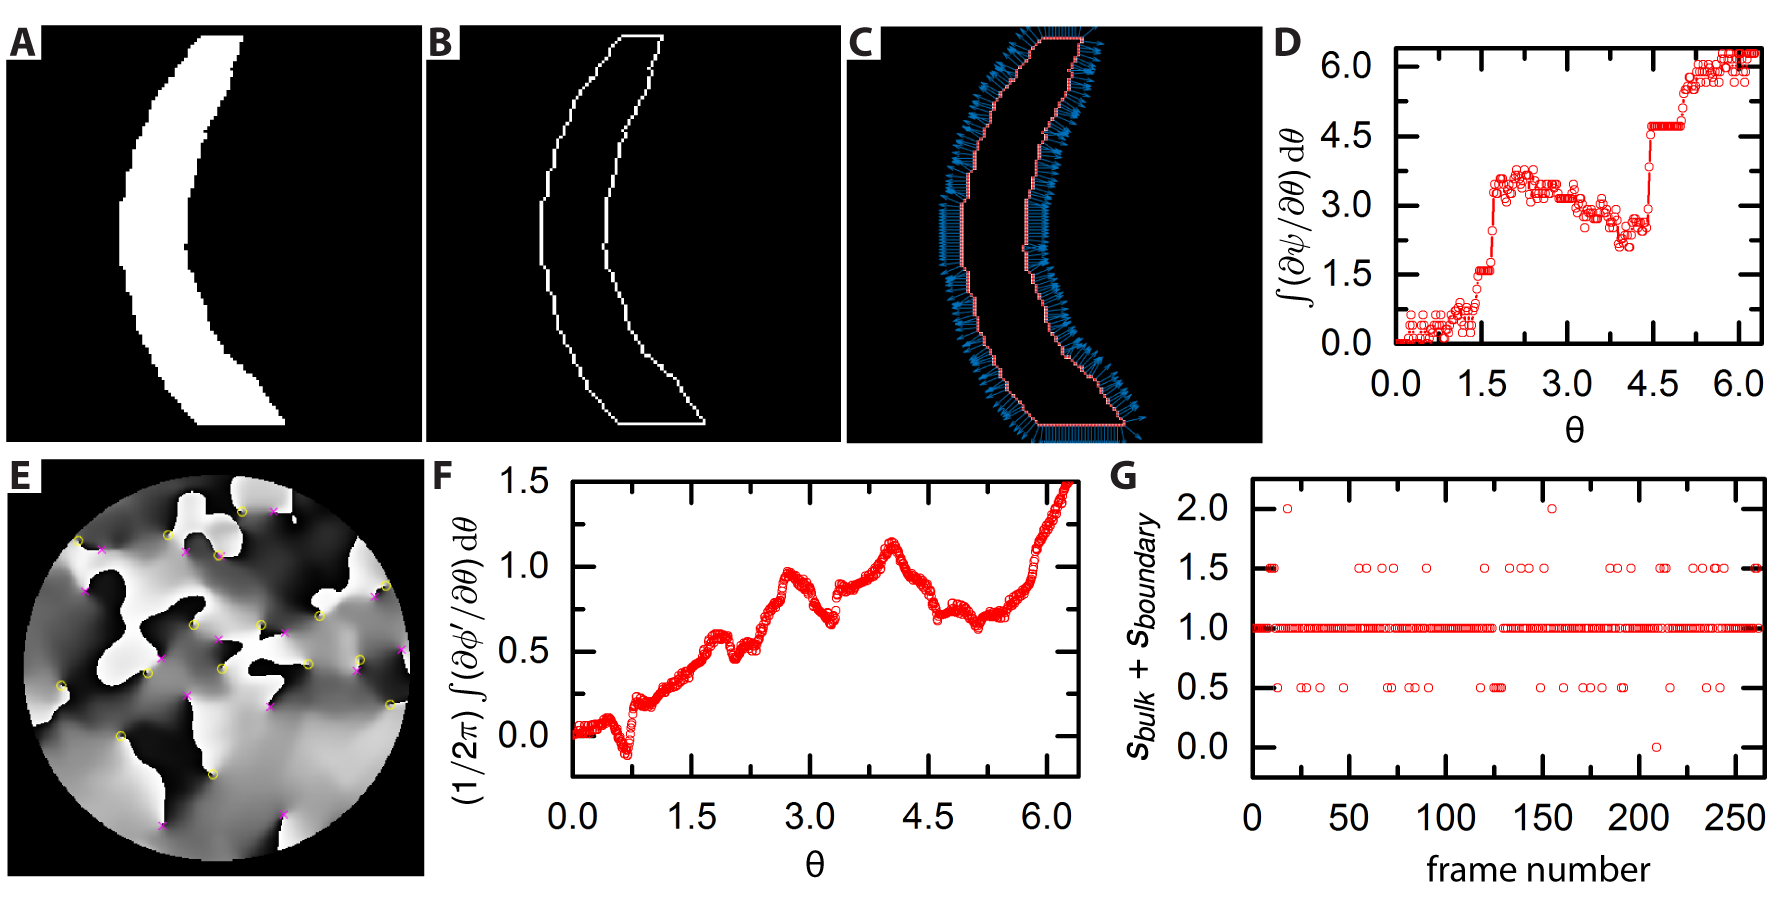
\includegraphics{figures/C3/Ch3-Figs_EdgeChargeErr.png}
  \caption{Boundary charge and defect detection error on active nematic toroids.
  (A-D), Validation of the Frenet-Serret frame.
  For the example mask in (A), we find the (B) boundary, estimate the unit tangent vectors, and then rotate the tangent vectors by $-\pi/2$ to get the (C) unit normal vectors and complete the Frenet-Serret frame.
  The image in (C) is zoomed in on the highlighted portion of (B) to better show the arrows.
  (D), We check the Frenet-Serret frame in (C) by integrating the change in the unit normal vector along the boundary, $\int\limits_{0}^{\theta} \textrm{d}(\psi - \pi/2) = \int\limits_{0}^{\theta} \textrm{d}\psi = \int\limits_{0}^{\theta} (\partial \psi/\partial \theta') \textrm{d}\theta'$, and see that the integral goes to $2 \pi$, as desired.
  (E), Circular region containing a director field from an active nematic toroid with $s = \pm 1/2$ defects found with our algorithm and labeled by (${\color{magenta} \times}$), (${\color{yellow} \circ}$), respectively, giving $s_{bulk} = \sum_i s_i = -1/2$.
  (F), $\int\limits_{\theta = 0}^{2\pi} \textrm{d}\phi'$ along the boundary yields $s_{boundary} = 3/2$ as $\theta \rightarrow 2 \pi$.
  (G), $s_{bulk} + s_{boundary}$ for 262 frames evaluated using the region in (A) applied to a torus with $\xi = 2.4$ and $a = 268$ $\upmu$m.
  There are 55 frames with $s_{bulk} + s_{boundary} \neq 1$ and 207 frames with $s_{bulk} + s_{boundary} = 1$, leading to $P(error) = 0.21$ and mean$(error) = 0.004$.}\label{f:3-EdgeChargeErr}
\end{figure}

We test our routine by first integrating the normal vectors along $\partial \Theta$, as shown in Figure~\ref{f:3-EdgeChargeErr}(D), finding $\oint_{\partial \Theta} \textrm{d}(\psi-\pi/2) = \oint_{\partial \Theta} \textrm{d}\psi = 2\pi$, as desired.
We now consider a small circular region and validate the algorithm using director fields from our active nematic toroids, as shown in the example in Figure~\ref{f:3-EdgeChargeErr}(E).
From the defects found by our algorithm, with $s = +1/2$ defects indicated by (${\color{magenta} \times}$) and $s = -1/2$ defects indicated by (${\color{yellow} \circ}$) in the example image in Figure~\ref{f:3-EdgeChargeErr}(E), we calculate $s_{bulk}= \sum\limits_i s_i=-1/2$.
Plotting $\oint_{\partial \Theta} \textrm{d}\phi'$ for the example in Figure~\ref{f:3-EdgeChargeErr}(E) in Figure~\ref{f:3-EdgeChargeErr}(F), we see that $s_{boundary} = 3/2$, resulting in $s_{bulk}+s_{boundary} = 1$, as required.

We now consider a region in the intensity projection for a torus and monitor  $s_{bulk}$ and $s_{boundary}$ over time.
For the example region in Figure~\ref{f:3-EdgeChargeErr}(A), we plot $s_{bulk}+s_{boundary}$ for every time frame in Figure~\ref{f:3-EdgeChargeErr}(G).
We see in this example that 55 frames out of 262 frames have an error; however, the error is typically only $\pm 1/2$, with only three frames having an error of $\pm 1$.
Calulating ${\rm mean}(error) = {\rm mean}(s_{bulk}(t) + s_{boundary}(t) - 1)$, for Figure~\ref{f:3-EdgeChargeErr}(G), we have ${\rm mean}(error) = [26(1/2) + 26(-1/2) + 2(1) + 1(-1)]/262 = 0.004$.
Importantly, since $|{\rm mean}(error)| \ll 1/2$, we see that the error in our analysis is random and we can trust the time-averaged topological charge.




\section{Measuring surface curvature}
From $h(x,y)$, we wish to calculate the Gaussian curvature of the surface.
Recall from Chapter~\ref{c:2} that $K = \textup{det} \big \{ \mathbf{L} \big \}$.
Thus, we need to calculate the Weingarten matrix.


\subsection{The Weingarten matrix}
For a smooth surface $\mathbf{R} = \{x, y, h(x,y)\}$, it is straightforward to use differential geometry and directly calculate the Weingarten matrix.
Note, however, that our surfaces are discrete and noisy and thus taking first and second derivatives is not obvious.
To avoid this, we rearrange Eq.~\ref{e:2-WeingartenMatrix} and notice that the Weingarten matrix relates a displacement in the tangent plane of a surface with the corresponding change in the unit normal vector along the displacement via,
\begin{equation}
  \begin{pmatrix}
  [(\hat{e}_1 \cdot \nabla) \mathbf{k}] \cdot \Delta \mathbf{r} \\
  [(\hat{e}_2 \cdot \nabla) \mathbf{k}] \cdot \Delta \mathbf{r}
  \end{pmatrix}
  =
  -\mathbf{L}
  \begin{pmatrix}
  \Delta \bm{r} \cdot \hat{e}_1 \\
  \Delta \bm{r} \cdot \hat{e}_2
  \end{pmatrix}\label{e:3-Kfit1}
\end{equation}
%(\hat{e}_j \cdot \nabla) \mathbf{k} \cdot \Delta \mathbf{r} = -\tensor{L}{_{ij}} \hat{e}_i \cdot \Delta \mathbf{r},
where $\hat{e}_i$ with $i = 1,2$ is an orthonormal basis in the tangent plane, $\mathbf{k}$ is the unit normal vector, and  $\mathbf{\Delta r} = \Delta r_j \hat{e}_j$ is an arbitrary displacement in the tangent plane.
Note that the relation, $(\hat{e}_j \cdot \nabla) \mathbf{k} = -\tensor{L}{_{ij}} \hat{e}_i$, Weingarten's formula, comes from the fact that the change in the surface normal due to infinitesimal displacements in the tangent plane is also in the tangent plane~\cite{RN35}.

Thus, for a point of interest on the surface, we can consider local displacement vectors and the corresponding change in the unit surface normal and then fit $\tensor{L}{_{ij}}$ according to Eq.~\ref{e:3-Kfit1} using an iteratively-reweighted least squares (IRLS) routine~\cite{RN32,RN31}.
This technique allows us to characterize a noisy surface without taking a discrete derivative and without any prior knowledge about the surface features.
In addition, an IRLS routine is a robust fit able to reject outliers and accommodate the noise in our data.


\subsection{Iteratively-reweighted least squares}
Consider a set of observations of a random variable where each observation is denoted by $y_{(i)}$ and is associated with a random variable $x_{(i)}$.
Given a model $y'_{(i)} = g(x_{(i)},\bm{\alpha})$, where $\bm{\alpha}$ is the parameter vector for the model, we can define the error of the model for each observation by the residual, $\gamma_{(i)} = y_{(i)} - y'_{(i)} = y_{(i)} - g(x_{(i)},\bm{\alpha})$.
A least-squares fit works to find the $\bm{\alpha}$ that minimizes the sum of the squared residuals:
\begin{equation}
  \argmin_{\bm{\alpha}} \sum\limits_i\,  \gamma_{(i)}^2.\label{e:3-LeastSquare}
\end{equation}
If the model is linear, the fit has an analytic solution~\cite{RN269}.
In addition, for normally-distributed data, the result of least-squares fit gives the maximum-likelihood values of $\bm{\alpha}$~\cite{RN269}.

However, since the cost of an error in a least squares fit scales quadratically with the size of the error, outliers can have a disproportionate effect on the final fit.
In fact, extreme outliers are often referred to as lever points for this exact reason.

One way to treat noisy or uncertain data is to assign a weight to each data point such that data points with larger error are weighted less.
The fit then becomes:
\begin{equation}
  \argmin_{\bm{\alpha}} \sum\limits_{(i)}\, (w_i \gamma_{(i)})^2,
\end{equation}
where $w_{(i)}$ is the weight associated to the observation $y_{(i)}$.
A weighted linear least-squares fit of this type is still analytically solvable~\cite{RN269}.
Unfortunately, weighted least-squares is still very sensitive to outliers if it is not obvious \emph{a priori} which data are the outliers.

Instead, we can construct a fit that is inherently less sensitive to outliers by replacing the square of the residual with a general cost function:
\begin{equation}
  \argmin_{\bm{\alpha}} \sum\limits_{(i)}\,\mathit{cost}(\gamma_{(i)}),\label{e:3-GeneralCostFit}
\end{equation}
such that the fit can deprioritize or even reject entirely large sources of error.
These cost functions are known as maximum-likelihood-type estimators, or M-estimators~\cite{RN269}.
Note that choosing the cost function $\mathit{cost}(\gamma_{(i)}) = \gamma_{(i)}^2$ gives a regular least-squares fit.
Unfortunately, a general cost function is not often analytically solvable or easy to minimize.
However, provided the cost function is differentiable, we can solve Eq.~\ref{e:3-GeneralCostFit} with an iteratively-reweighted least-squares (IRLS) process.

To do this, we need to recast Eq.~\ref{e:3-GeneralCostFit} in terms of a weighted least-squares fit.
We start by taking the derivative of Eq.~\ref{e:3-GeneralCostFit} with respect to $\alpha_j$:
\begin{equation}
  \sum\limits_i\,\frac{\partial \, \mathit{cost}(\gamma_{(i)})}{\partial \gamma_{(i)}} \frac{\partial \gamma_{(i)}}{\partial \alpha_j} = 0.\label{e:3-IRLSderiv1}
\end{equation}
Notice that if we define a weight function like $w(\gamma_{(i)}) = \dfrac{1}{\gamma_{(i)}}\dfrac{\partial \, \mathit{cost}(\gamma_{(i)})}{\partial \gamma_{(i)}}$, we can re-write Eq.~\ref{e:3-IRLSderiv1} as:
\begin{equation}
  \sum\limits_{(i)}\,w(\gamma_{(i)}) \gamma_{(i)} \frac{\partial \gamma_{(i)}}{\partial \alpha_j} = 0.\label{e:3-IRLSderiv2}
\end{equation}
 Solving Eq.~\ref{e:3-IRLSderiv2} for $\bm{\alpha}$ is equivalent to minimizing:
 \begin{equation}
   \argmin_{\bm{\alpha}} \sum\limits_i\,\big \{ (w_{(i)}(\gamma_{(i)}) \gamma_{(i)}(\bm{\alpha}))^2 \big \},\label{e:3-WeightLS}
 \end{equation}
 a weighted least-squares fit, as desired.
Hence, solving Eq.~\ref{e:3-GeneralCostFit} is equivalent to solving a weighted least-squares fit, where we have expressed $\gamma_{(i)}$ inside the minimization as an explicit function of $\bm{\alpha}$ for clarity.
Since our weights are dependent on the residuals, we solve Eq.~\ref{e:3-WeightLS} iteratively, where the weights for an iteration $(p)$ are determined by the residuals from the previous iteration, giving:
\begin{equation}
  \bm{\alpha}^{(p+1)} = \argmin_{\bm{\alpha}} \sum\limits_i\,\bigg \{ \bigg [w_{(i)} \big(\gamma_{(i)}^{(p)}\big ) \gamma^{(p+1)}_{(i)}(\bm{\alpha}) \bigg ]^2 \bigg \},
\end{equation}
where $w_{(i)} \big(\gamma_{(i)}^{(p)}\big )$ are the weights calculated using the residuals for iteration $p$.
The weights for a given iteration are constants and do not change during the minimization.
With enough iterations, the $\gamma_{(i)}$ converge and we have the $\bm{\alpha}$ values that solve Eq.~\ref{e:3-WeightLS}.
The entire process can be described by the recursion relation:
\begin{align}
  \gamma_{(i)}^{(p+1)}
  &= y_{(i)} - g\big (x_{(i)},\bm{\alpha}^{(p+1)}\big ) \nonumber \\
  &= y_{(i)} - g\Bigg (x_{(i)}, \argmin_{\bm{\alpha}} \sum\limits_i\,\bigg \{ \bigg [w_{(i)} \big(\gamma_{(i)}^{(p)}\big ) \gamma^{(p+1)}_{(i)}(\bm{\alpha}) \bigg ]^2 \bigg \} \Bigg).
\end{align}

Since these cost functions do not need to be everywhere convex, they may not necessarily have a global minimum, or even a guaranteed convergence.
However, those that are not globally convex often deal with large error more severely than convex functions.
Thus, to get the best of both worlds, we will first fit our surface using a convex M-estimator until the fit converges and then fit the output of the convex M-estimator with a globally non-convex M-estimator.
Following Ref.~\cite{RN31}, we use the convex ``Fair'' M-estimator and the non-convex ``Geman-McClure'' (GMC) M-estimator~\cite{RN52}, where the functional forms of the cost function and weight functions are provided in Table~\ref{t:3-CostFxn} and plotted in Figure~\ref{f:3-CostFxn}.
Both the GMC and the Fair M-estimator have a tuning constant, $c$, that adjusts the influence of errors on the fitting weights for the next iteration; decreasing $c$ reduces the influence of large residuals.
This can be seen by considering the blue and red curves in Figure~\ref{f:3-CostFxn}(B--D), where $c_{blue} = 2c_{red}$.
Notice how increasing $c$ causes the weights for large residuals to increase; data with a large residual have more influence in the blue curves than in the red curves.

This raises the question of how to compare different M-estimators and how to choose a value for the tuning parameters.
One way to do this is to test an M-estimator with some tuning parameter using data drawn from a Gaussian with zero mean and unit variance, the standard normal distribution.
For example, let the model $g(x_{(i)},\bm{\alpha})$ estimate the mean of the distribution given the input $x$.
The residuals are $\gamma_{(i)} = 0 - g(x_{(i)},\bm{\alpha})$, such that the sample variance is $(1/N)\sum_i^N \gamma_{(i)}^2$ and the variance of the mean is $(1/N^2)\sum_i^N \gamma_{(i)}^2 = (1/N)\sum_i^N \gamma_{(i)}^2/N$.
Notice that if our model just returns the value of the observation, $g(x_{(i)},\bm{\alpha}) = x_{(i)}$, then we recover the well-known formulas for both the sample variance $(1/N)\sum_i^N x_{(i)}^2$, and sample variance of the mean $(1/N)\sum_i^N x_{(i)}^2/N$.
We compare the sample variance of the mean from the model $g(x_{(i)},\bm{\alpha})$ versus that from the observation itself $x_{(i)}$ in the limit that $N \to \infty$ via the asymptotic relative efficiency (ARE):
\begin{align}
  ARE &= \lim_{N \to \infty} \frac{(1/N)\sum\limits_i^N x_{(i)}^2/N}{(1/N)\sum\limits_i^N \gamma_{(i)}^2/N}\\
  &= \frac{\lim_{N \to \infty} \sum\limits_i^N x_{(i)}^2}{\lim_{N \to \infty} \sum\limits_i^N \gamma_{(i)}^2}\\
  &= \frac{N}{\lim_{N \to \infty} \sum\limits_i^N \gamma_{(i)}^2},
\end{align}
where we have taken advantage of the fact that $\lim_{N \to \infty} (1/N)\sum_i^N x_{(i)}^2 = 1$, the true variance for the standard normal distribution.

We see that if $g(x_{(i)},\bm{\alpha})$ produces a variance of the mean of $1/N$, the ARE will be unity, or 100\%.
Similarly, if $g(x_{(i)},\bm{\alpha})$ produces a smaller variance of the mean, the efficiency will be greater than 100\%.
The ARE thus can be used to give context to an estimator with a set of input parameters.
We note that the literature generally quotes parameters for their M-estimators that have 95\% ARE; the red curves in Figure~\ref{f:3-CostFxn}(B--D) were computed with these values~\cite{RN318,RN32,RN52}.
\newpage
\begin{table}[ht]
  \centering
  \caption{Cost and weight functions of common M-estimators.\@ $x$ are the residuals and $c$ is a tuning parameter.}
  \begin{tabular}{|r c c |}
    \hline \\[-0.45cm]
     & $\mathit{cost}(x)$ & $w(x)$\\
    \hline \\[-0.3cm]
    {\bf least-squares}:& $\dfrac{x^2}{2}$ & 1\\ [0.5cm]
    {\bf L$_p$}:& $ \dfrac{|x|^p}{p} $ & $|x|^{p-2}$\\[0.5cm]
    {\bf Fair}:& $c^2 \Bigg [ \dfrac{|x|}{c} - \log \Big ( 1 + \dfrac{|x|}{c}\Big ) \Bigg ]$ & $\dfrac{1}{1 + |x|/c}$ \\ [0.5cm]
    {\bf Geman-McClure}:& $\dfrac{(x/c)^2}{1+(x/c)^2}$ & $\dfrac{2}{(1+(x/c)^2)^2}$ \\ [0.5cm]
    {\bf Cauchy}:& $\dfrac{c^2}{2} \log \big ( 1 + (x/c)^2 \big)$ & $\dfrac{1}{1 + (x/c)^2}$\\ [0.5cm]
    \hline
  \end{tabular}\label{t:3-CostFxn}
\end{table}

\begin{figure}[H]
  \centering
  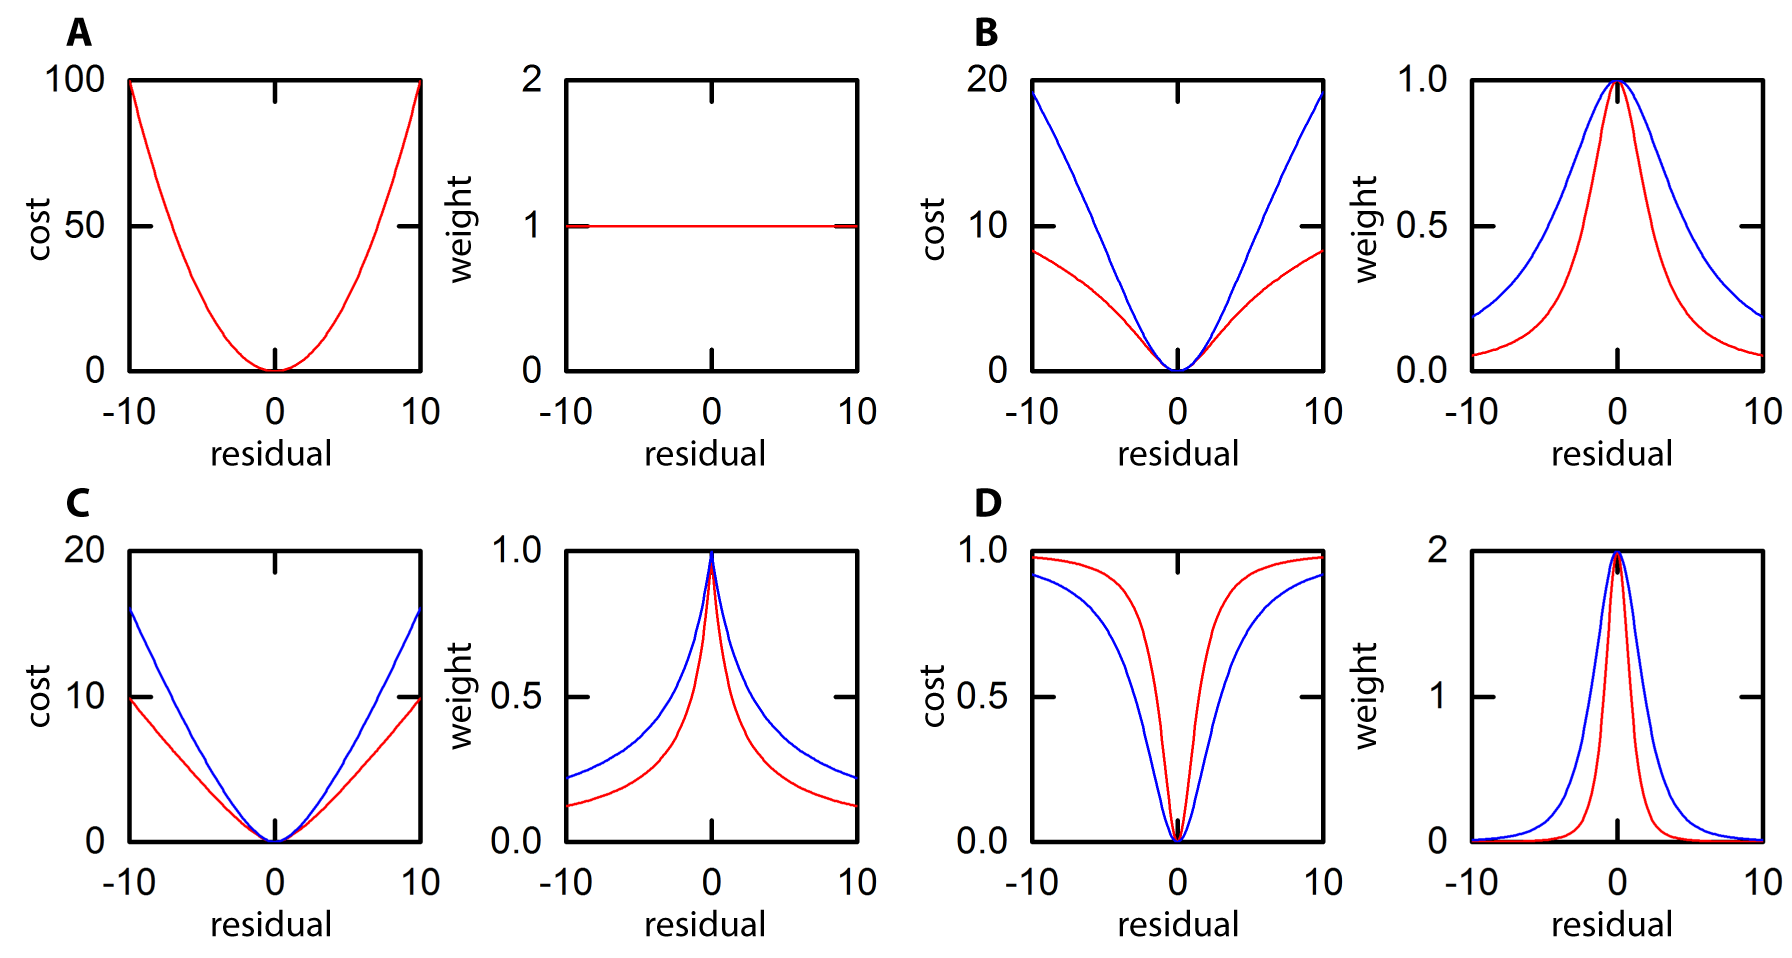
\includegraphics{figures/C3/Ch3-Figs_IRLSfxn.png}
  \caption{Plots of the cost functions and weight functions for common M-estimators.
  (A) The cost and weight function for a least-squares fit.
  (B-D) The cost and weight functions for a (B) Cauchy M-estimator, a (C) Fair M-estimator, and a (D) GMC M-Estimator, with the tuning parameter for the red curves set to yield 95\% efficiency on a standard normal, and the tuning parameter for the blue curve set to twice the value in the red curve.
  The least-squares estimator in (A) and the Fair estimator in (C) have everywhere convex cost functions, in contrast to the Cauchy and the GMC M-estimators in (B,D), respectively.}\label{f:3-CostFxn}
\end{figure}
\newpage
\subsection{Fitting the Weingarten matrix on a surface}
From a Monge parameterization $h(x,y)$ of a surface~\cite{RN35,RN23}, we start by computing the Delauney triangulation~\cite{RN34} such that every point or pixel in $h(x,y)$ is a vertex in the triangulation.
From the triangulation, we estimate $\mathbf{k}$ at every vertex as the average of the unit normals of the adjacent faces.
Once we have a triangulation and the $\mathbf{k}$ estimates, we proceed to fit the curvature.

Let $\mathbf{R}_{[0]}$ be an example point of interest with normal $\mathbf{k}_{[0]}$.
We first make an initial fit using regular least-squares to serve as an input into the IRLS routine.
We consider all points within a distance $d_1$ of $\mathbf{R}_{[0]}$ to be within the region of interest and then use $\mathbf{k}_{[0]}$ to transform the region of interest into the tangent plane at $\mathbf{R}_{[0]}$.
This step allows us to characterize the surface locally in terms of an orthonormal basis $\{\hat{e}_1,\hat{e}_2,\mathbf{k}\}$, where $\hat{e}_1$ and $\hat{e}_2$ are in the tangent plane.
We then calculate the displacement vectors in the tangent plane $\Delta \mathbf{R}_{[i,j]} = \mathbf{R}_{[j]}-\mathbf{R}_{[i]}$ and the change in the unit normal $\Delta \mathbf{k}_{[i,j]} = \mathbf{k}_{[j]}-\mathbf{k}_{[i]}$ for every possible pair of points in the region of interest, with individual points indexed with $i$ and $j$.
Importantly, as depicted in Figure~\ref{f:3-CurvFitSchem}, the pairs of points do not need to include $\mathbf{R}_{[0]}$; this reduces the influence of error in $\mathbf{R}_{[0]}$ and $\mathbf{k}_{[0]}$.
Since we are considering how $\mathbf{k}$ changes along $\Delta \mathbf{R}$, a finite displacement vector, $\Delta \mathbf{k}$ is not generally in the tangent plane.
Thus, we need to extend the Weingarten Matrix to consider the component of $\Delta \mathbf{k}$ along $\mathbf{k}$~\cite{RN31,RN32}:
\begin{equation}
\begin{pmatrix}
\Delta \mathbf{k} \cdot \hat{e}_1 \\
\Delta \mathbf{k} \cdot \hat{e}_2 \\
\Delta \mathbf{k} \cdot \mathbf{k}_0
\end{pmatrix}
=
\bm{\Lambda}
\begin{pmatrix}
\Delta \bm{R} \cdot \hat{e}_1 \\
\Delta \bm{R} \cdot \hat{e}_2
\end{pmatrix}
=
\begin{pmatrix}
\tensor{L}{_1_1} & \tensor{L}{_1_2} \\
\tensor{L}{_2_1} & \tensor{L}{_2_2} \\
M_{1} & M_{2}
\end{pmatrix}
\begin{pmatrix}
\Delta \bm{R} \cdot \hat{e}_1 \\
\Delta \bm{R} \cdot \hat{e}_2
\end{pmatrix},
\label{e:3-Kfit2}
\end{equation}
where we have added $M_1$ and $M_2$ to $\mathbf{L}$ to form $\bm{\Lambda}$, the extended Weingarten Matrix.
This additional information will eventually allow us to re-estimate $\mathbf{k}$~\cite{RN31}.
\begin{figure}
  \centering
  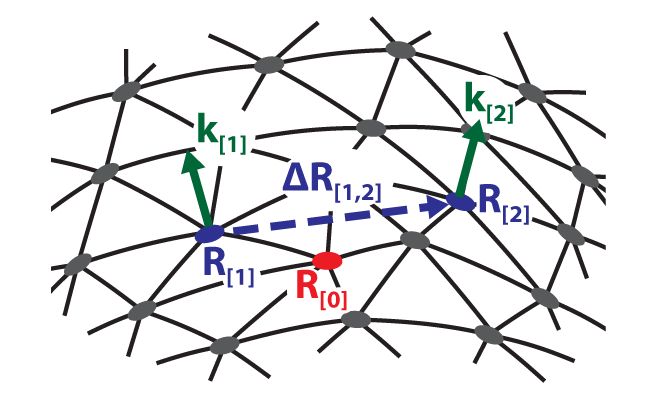
\includegraphics{figures/C3/Ch3-Figs_CurvFitSchem.png}
  \caption{Schematic of the quantities used to calculate the Gaussian curvature of a triangulated surface.
  $\mathbf{R}_{[0]}$ is the point of interest.
  $\mathbf{R}_{[1]}$ and $\mathbf{R}_{[2]}$ are an example pair of points close to the point of interest with $\Delta \mathbf{R}_{[1,2]} = \mathbf{R}_{[2]}-\mathbf{R}_{[1]}$ the displacement vector in the tangent plane of $\mathbf{R}_{[0]}$.
  $\mathbf{k}_{[1]}$ and $\mathbf{k}_{[2]}$ are the unit surface normal vectors associated to $\mathbf{R}_{[1]}$ and $\mathbf{R}_{[2]}$.}\label{f:3-CurvFitSchem}
\end{figure}

We now have a system of three equations to fit with 5 parameters, as $\tensor{L}{_{12}} = \tensor{L}{_{21}}$.
If we naively expand Eq.~\ref{e:3-Kfit2} directly into three equations,
\begin{align}
  \Delta k_1 &= \tensor{L}{_{11}} \Delta R_1 + \tensor{L}{_{12}} \Delta R_2\label{e:3-KfitNaiveA} \\
  \Delta k_2 &= \tensor{L}{_{21}} \Delta R_1 + \tensor{L}{_{22}} \Delta R_2\label{e:3-KfitNaiveB} \\
  \Delta k_k &= M_1 \Delta R_1 + M_2 \Delta R_2,\label{e:3-KfitNaiveC}
\end{align}
where we have expanded the vectors like $\mathbf{v}\cdot \hat{e}_i = v_i$ and $\Delta k_k$ refers to the component of $\Delta \mathbf{k}$ along the surface normal, we see that $\tensor{L}{_{12}}$ will be determined entirely by the variation along $\hat{e}_2$, and $\tensor{L}{_{11}}$ by the variation along $\hat{e}_1$.
The result of $\tensor{L}{_{12}}$ from fitting Eq.~\ref{e:3-KfitNaiveA} will then set the value of $\tensor{L}{_{21}}$ in the fit of Eq.~\ref{e:3-KfitNaiveB} so that only $\tensor{L}{_{22}}$ is free to vary during the fit.
This means that in principle, the choice of $\hat{e}_i$ could affect the output curvature.
To account for this, we manipulate Eqs.~\ref{e:3-KfitNaiveA}--\ref{e:3-KfitNaiveC} to be:
\begin{align}
  \Delta k_2 \Delta R_2 - \Delta k_1 \Delta R_1 &= (\Delta R_2)^2 \tensor{L}{_{22}} - (\Delta R_1)^2 \tensor{L}{_{11}}\label{e:3-KfitConstrainedA}\\
  \Delta k_1 + \Delta k_2 - \tensor{L}{_{11}} \Delta R_1 - \tensor{L}{_{22}} \Delta R_2 &= (\Delta R_1 + \Delta R_2)\tensor{L}{_{12}}\label{e:3-KfitConstrainedB}\\
  \Delta k_k &= M_1 \Delta R_1 + M_2 \Delta R_2.\label{e:3-KfitConstrainedC}
\end{align}
If we do the fits in Eqs.~\ref{e:3-KfitConstrainedA}--\ref{e:3-KfitConstrainedC} in order, the values of $\tensor{L}{_{11}}$ and $\tensor{L}{_{22}}$ from fitting Eq.~\ref{e:3-KfitConstrainedA} are inserted as fixed parameters into the fit of Eq.~\ref{e:3-KfitConstrainedB}.
However, now the values of $\tensor{L}{_{ij}}$ are determined by the variation in both directions in the tangent plane.
Once we have estimates of the elements of $\bm{\Lambda}$ from the initial least-squares fit, we move on to fitting the curvature with the IRLS routine.

We now choose all points within a distance $d_2$ of $\mathbf{R}_{[0]}$, where $d_2 > d_1$, and as before, transform into the tangent plane and calculate the associated $\mathbf{\Delta k}_{[i,j]}$ and $\mathbf{\Delta R}_{[i,j]}$ between all pairs of points.
In addition, we calculate a geometric weight for each $\mathbf{\Delta R}_{[i,j]}$:
\begin{equation}
  m_{(ij)} = \frac{\textrm{C}} {\mathbf{\Delta R}_{[0,i]}^2 + \mathbf{\Delta R}_{[0,j]}^2},
\end{equation}
where $\textrm{C}$ is a normalization constant such that $\sum\limits_{i,j} m_{(ij)} = 1$.
The geometric weight ensures that data far from $\mathbf{R}_{[0]}$ contribute less to the curvature at $\mathbf{R}_{[0]}$~\cite{RN32,RN31}.
We then pass the $\mathbf{\Delta k}_{[i,j]}$, the $\mathbf{\Delta R}_{[i,j]}$, the $m_{[i,j]}$, the initial values in $\bm{\Lambda}$, the appropriate tuning parameters, and a convergence tolerance to our IRLS routine.
Our routine starts by calculating the residuals using $\bm{\Lambda}$ from the previous fit like:
\begin{equation}
  \gamma_{(ij)}^{(p)} = \sqrt{|\mathbf{\Delta k}_{[i,j]}- \bm{\Lambda}^{(p)} \mathbf{\Delta R}_{[i,j]}|^2},
\end{equation}
where $p$ is the iteration number and the $0^{\textrm{th}}$ iteration refers to the initial least-squares fit.
The routine then calculates the weights for the Fair M-estimator seen in Table~\ref{t:3-CostFxn}, multiplies the Fair weights for each pair of points with the associated $m_{(ij)}$ to get the final fitting weight, performs a weighted least-squares fit of Eqs.~\ref{e:3-KfitConstrainedA}--\ref{e:3-KfitConstrainedC}, and then repeats the process from the beginning until the fit converges.
For the Fair fit we take the tuning constant $c_F^{(p+1)} = c_F^{initial} \, \textrm{median}\{ \bm{\gamma}^{(p)} \}$, where $p$ is the iteration number, $\bm{\gamma}^{(p)}$ is a vector of the residuals, and $c_F^{initial}$ is an input parameter.
We include the median of the residuals in our tuning constant so that the tuning parameter in the fit doesn't need to be adjusted as much between datasets with different levels of noise.
In this case, we use the median of the residuals, as the mean can be distorted by large errors.
The Fair fit converges when the cost function changes by less than the specified convergence tolerance between subsequent iterations.
While we set an upper limit of 50 iterations for the Fair fit, the fit typically converges in fewer than 20 iterations taking the convergence tolerance to be 0.001.

The final values of $\bm{\Lambda}$ from the Fair fit are then used as the initial values for an IRLS fit using a GMC M-estimator.
The overall flow of the algorithm is the same for the GMC M-estimator as it was for the Fair M-estimator.
However, there are some key differences in how the fitting weights are handled.
Here, it is possible to reject outliers by calculating the fitting weights as,
\begin{equation}
  w_{(ij)}^{(p+1)} =
\begin{cases}
0 & \text{if} \quad \gamma_{(ij)}^{(p)} > b \ c_{GMC}^{(p)} \\
 \dfrac{2}{(1+(\gamma_{(ij)}^{(p)} / c_{GMC}^{(p)})^2)^2} & \text{otherwise}
\end{cases},
\end{equation}
where $c_{GMC}^{(p)} = c_{GMC}^{initial} \, \textrm{median}\{ \bm{\gamma}^{(p)} \}$ is the tuning constant for the GMC fit, and $c_{GMC}^{initial}$ and $b$ are input parameters.
We have modified the standard GMC weight function to exclude data with a residual that is too large.
The outlier rejection works by comparing each residual against the median of the residuals.
The parameter $b$ then determines how much variance with respect to the median residual is allowed.
In addition, since the GMC fit is not guaranteed to converge, we ensure that the $c_{GMC}^{(p)} \leq c_{GMC}^{(0)}$ by setting iterations with $c_{GMC}^{(p)} > c_{GMC}^{(0)}$ to have $c_{GMC}^{(p)} = c_{GMC}^{(0)}$.

The GMC fit converges when the cost function changes by less than the specified convergence tolerance between subsequent iterations.
We set an upper limit of 20 iterations for the GMC fit, but the fit typically converges in fewer than 10 iterations when taking the convergence tolerance to be 0.001.
We display this entire IRLS fitting process for an example point, with the residuals, the weights, $\bm{\Lambda}$, and $K$ displayed for the Fair fit and the GMC fit in Figure~\ref{f:3-IRLSexample}(A,B), respectively.
The initial output of the least squares fit is passed to the Fair function and displayed as the 0$^{\rm th}$ iteration [Figure~\ref{f:3-IRLSexample}(A)].
Note how the {\it cost} changes largely between the 0$^{\rm th}$ and 2$^{\rm nd}$, but changes very little between the 2$^{\rm nd}$ and 4$^{\rm th}$ iterations [Figure~\ref{f:3-IRLSexample}(A)].
The Fair fit converges on the 4$^{\rm th}$ iteration; the values are then passed the GMC fit [Figure~\ref{f:3-IRLSexample}(B)].

In the subsequnt GMC fit displayed in Figure~\ref{f:3-IRLSexample}(B), the dashed line indicates the outlier rejection criterion; residuals above the dashed line have their weight set to 0.
Note how the ability to reject outliers lets the GMC fit in Figure~\ref{f:3-IRLSexample}(B) find a solution where a majority of the residuals are small.
Similar to the Fair fit, the cost in the GMC fit drops rapidly; by the 8$^{\rm th}$ iteration both the cost and the Gaussian curvature are very close to their final values [Figure~\ref{f:3-IRLSexample}(B)].
The GMC fit converges on the 10$^{th}$ iteration.
The routine outputs the GMC weights from the final fitting iteration and the final values of $\bm{\Lambda}$.
Finally, we calculate the Gaussian curvature of at $\mathbf{R}_{[0]}$ taking $K = \textup{det}\{ \mathbf{L} \}$ and move on to correcting $\mathbf{k}_{[0]}$.

\begin{figure}[H]
  \centering
  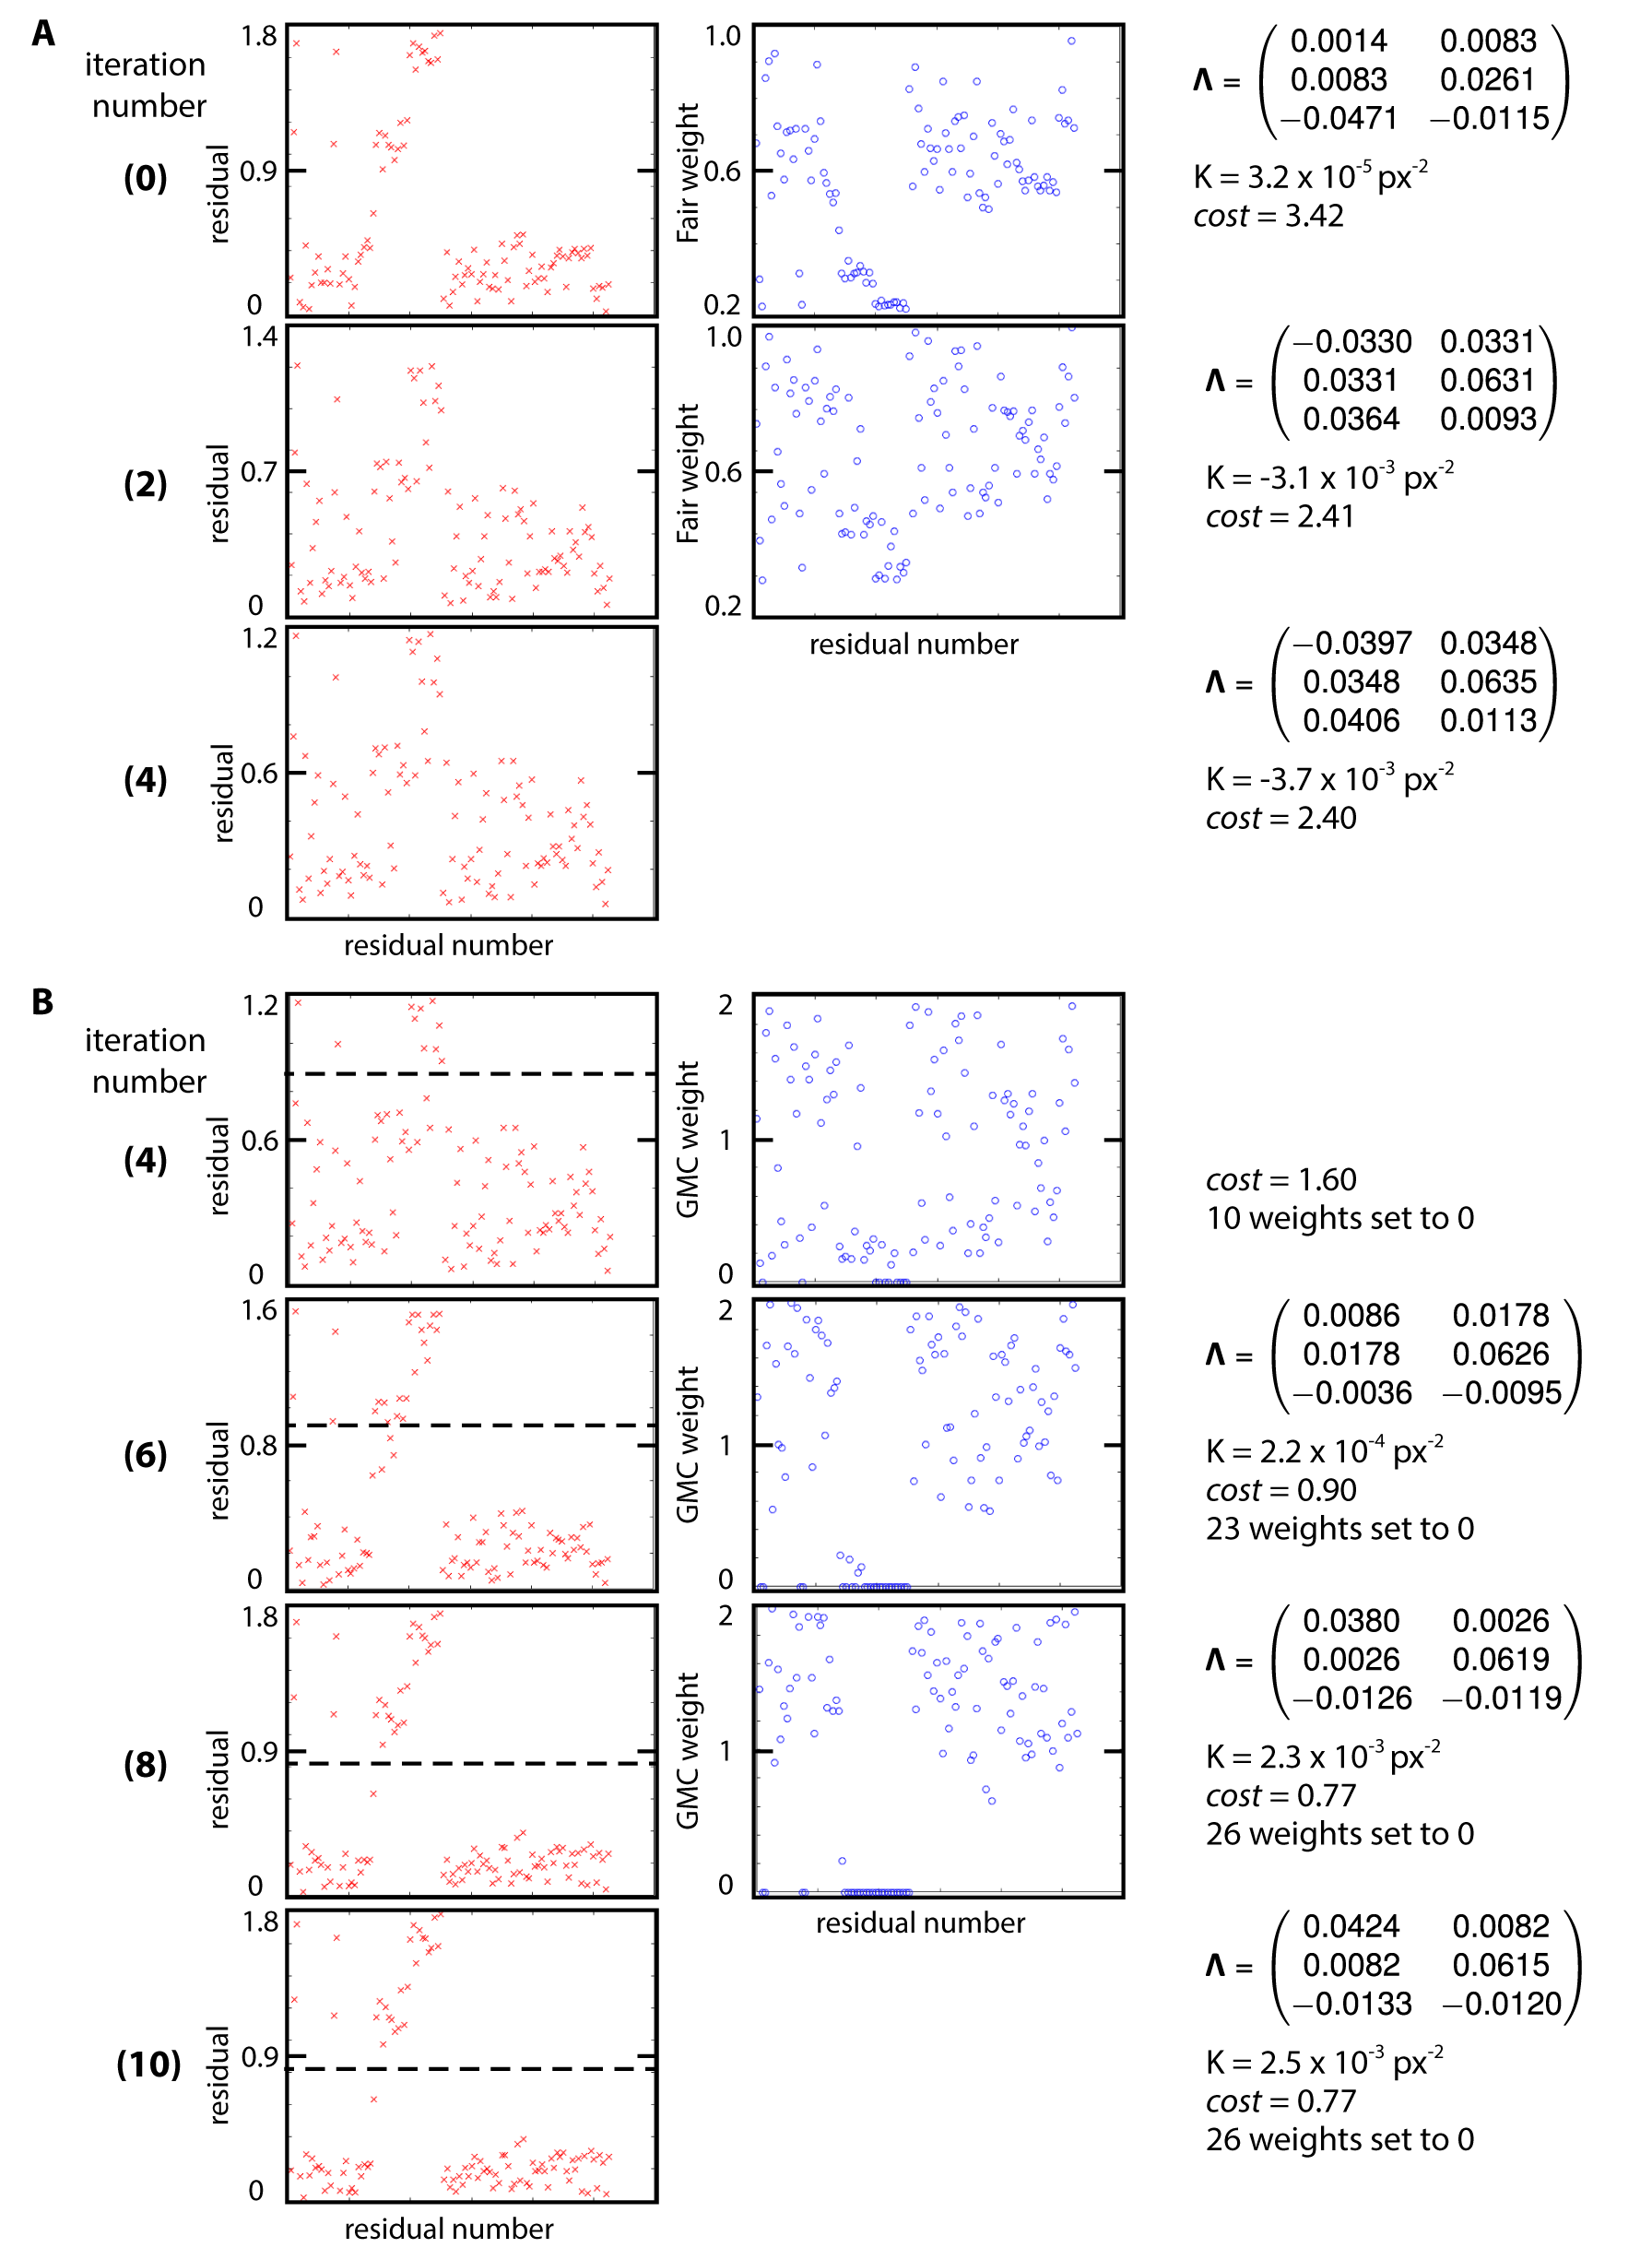
\includegraphics[scale=0.95]{figures/C3/Ch3-Figs_IRLSexample.png}
  \caption{Example IRLS fit of the curvature at a point on a surface.
  (A,B) Residuals, weights, $\bm{\Lambda}$, $K$, and cost for the (A) Fair M-estimator and (B) GMC M-estimator over multiple iterations, with the iteration number to the left of the residuals.
  The 0$^{\rm th}$ iteration corresponds to the output from the initial least-squares fit. The dashed line in (A) is the outlier rejection criterion; residuals above the line have their weight set to 0.}\label{f:3-IRLSexample}
\end{figure}

\subsection{Correcting the surface normal vectors}
We use the fitting weights from the final iteration $(p)$ and the final values in $\bm{\Lambda}$ to correct our initial estimate of $\mathbf{k}_{[0]}$ using a weighted average~\cite{RN31}:
\begin{equation}
\mathbf{k}_{[0]}^{(p)} = \frac{\sum\limits_i m_{(0i)}w_{(0i)}^{(p)}(\mathbf{k}_{[i]}^{(0)} - \mathbf{\Lambda}^{(p)}\mathbf{\Delta R}_{[0,i]})}{\sum\limits_j m_{(0j)}w_{(0j)}^{(p)}},
\end{equation}
where $\mathbf{k}_{[0]}^{(p)}$ corresponds to the re-estimated unit normal.
Note that here we have only used pairs of points that include $\mathbf{R}_{[0]}$.
This re-estimation uses the fitted curvature to determine what the surface normal should be.


\subsection{Finding the area element}
Once we have the re-estimated normal vectors everywhere on the surface, we can calculate the determinant of the metric~\cite{RN35},
\begin{equation}
g = \frac{1}{(\mathbf{k}^{(p)} \cdot \mathbf{\hat{z}})^2}.
\end{equation}
The determinant of the metric lets us connect areas in our flat intensity projection with areas on our curved toroidal surface via the local area element~\cite{RN35}, $\textrm{dA} = \sqrt{g} \, \textrm{dx}\textrm{dy}$.
Physically, we see that in the Monge parameterization, $\sqrt{g}$ reflects the tilt angle of the surface when compared to the flat plane that parameterizes the height of the surface.


\subsection{Validation on test surfaces}
We validate our routine on hemispheres and saddle-like surfaces with varying levels of random noise inserted into the height of the surface in order to mimic the noise in our confocal data.
We specify the noise as a percentage of the radii of curvature used to generate the test surface.
A surface without noise is insensitive to $d_1$, $d_2$, and the tuning constants in the fit.
This is shown for the noiseless hemisphere in Figure~\ref{f:3-CurvFitSphere}(A) with $K = 1.1 \times 10^{-3}$ px$^{-2}$, where the initial least-squares fit and the output of the IRLS fit are shown in Figure~\ref{f:3-CurvFitSphere}(B,C), respectively, and the color scale is displayed in Figure~\ref{f:3-CurvFitSphere}(I).
We test surfaces with up to 3\% noise; this is greater than the noise in our toroidal droplets.
We find that setting $b=2$ and $c_{F}^{initial} = 1.3998$ and $c_{GMC}^{initial}=1.4826$, their respective 95\% efficiency values~\cite{RN52,RN318}, works well.
In addition, we see that $d_2$ matters far more than $d_1$; increasing $d_2$ improves the noise tolerance of the fit.
\begin{figure}
  \centering
  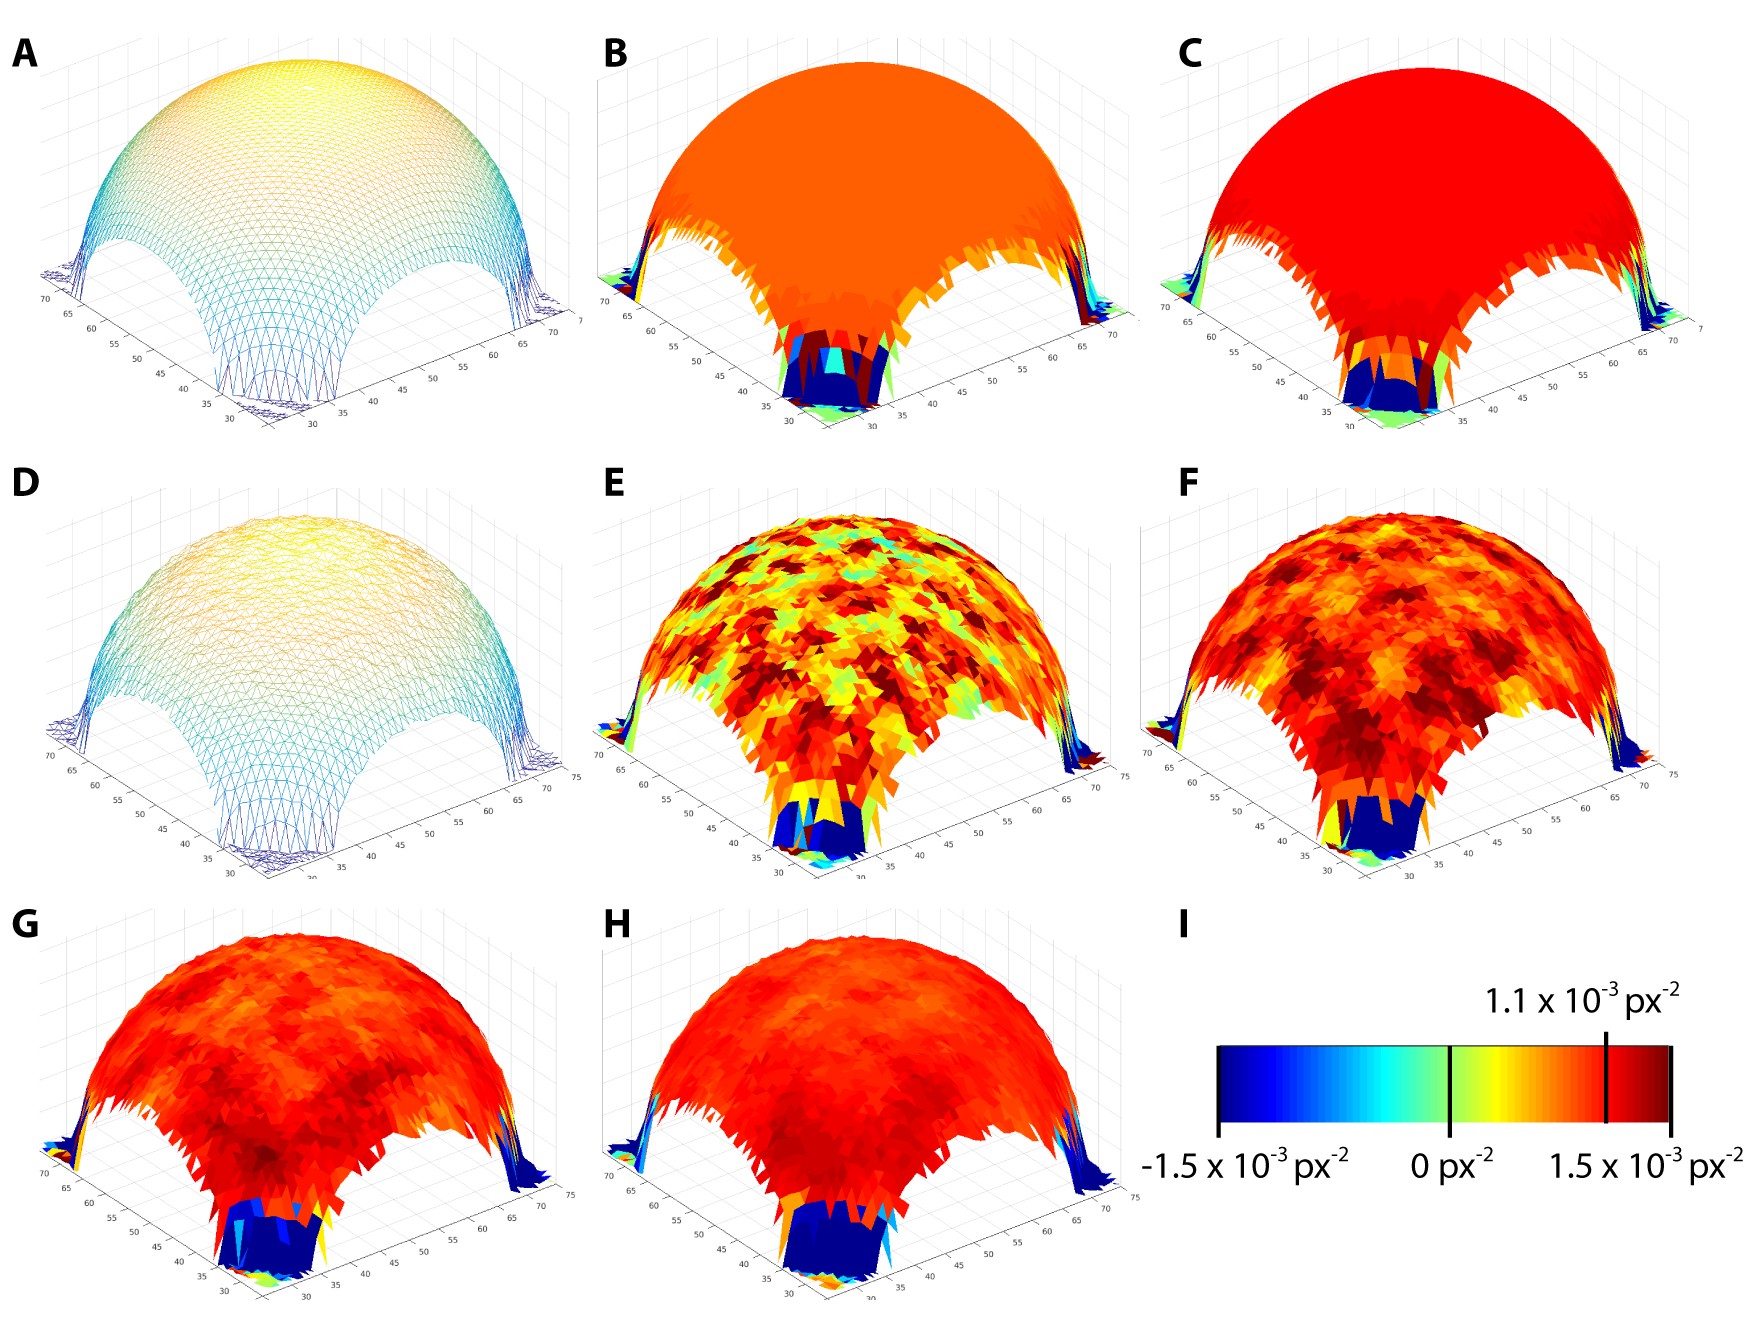
\includegraphics{figures/C3/Ch3-Figs_CurvFitSphere.png}
  \caption{Fitting the curvature of hemispheres with varying noise.
  (A-C) A hemisphere with $r = 30$ px and $K = 1.1 \times 10^{-3}$ px$^{-2}$ everywhere.
  The original triangulation is displayed in (A), the output of the initial least-squared fit with $d_1=2$ in (B), and the output of the IRLS fit with $d_2=4$ in (C), with the color scale for the curvature in (I).
  (D-H) The hemisphere in (A) with random noise from a distribution with mean 0 px and width 0.3 px added to the height at every point in the triangulation.
  The triangulation is displayed in (D), the output of the initial least-squared fit with $d_1=4$ in (E), and the output of the IRLS fit with $d_2=6,8,10$ in (F-H), respectively, with the color scale for the curvature in (I).}\label{f:3-CurvFitSphere}
\end{figure}

For a given amount of noise, we fit a test surface multiple times while increasing $d_2$ until the change in the curvature with increasing $d_2$ is small enough.
This process is illustrated for the example hemisphere with 1\% noise and an initial $K =1.1 \times 10^{-3}$ px$^{-2}$ displayed in Figure~\ref{f:3-CurvFitSphere}(D).
The output from the initial least-squares fit is shown in Figure~\ref{f:3-CurvFitSphere}(E) and the outputs from increasing values of $d_2$ are shown in Figure~\ref{f:3-CurvFitSphere}(F-H), where the color scale is displayed in Figure~\ref{f:3-CurvFitSphere}(I).
Note that $K$ does not change appreciably between $d_2 = 8$ in Figure~\ref{f:3-CurvFitSphere}(G) and $d_2 = 10$ in ~\ref{f:3-CurvFitSphere}(H).
For the final fitting parameters $d_1 = 4$ and $d_2 = 10$, we take the mean and standard deviation of $K$ everywhere on the surface, $\overbar{K} = 1.0 \times 10^{-3}$ px$^{2}$ and $\sqrt{\Delta K^2} = 0.1 \times 10^{-3}$ px$^{2}$.
This shows that the fit deals well with noise on the surface provided $d_2$ is large enough.
While we could in principle set $d_2$ to the size of the surface to eliminate this step, our fit runtime scales factorially with increasing $d_2$ such that we must balance runtime against improvements in the output curvature.
\begin{figure}
  \centering
  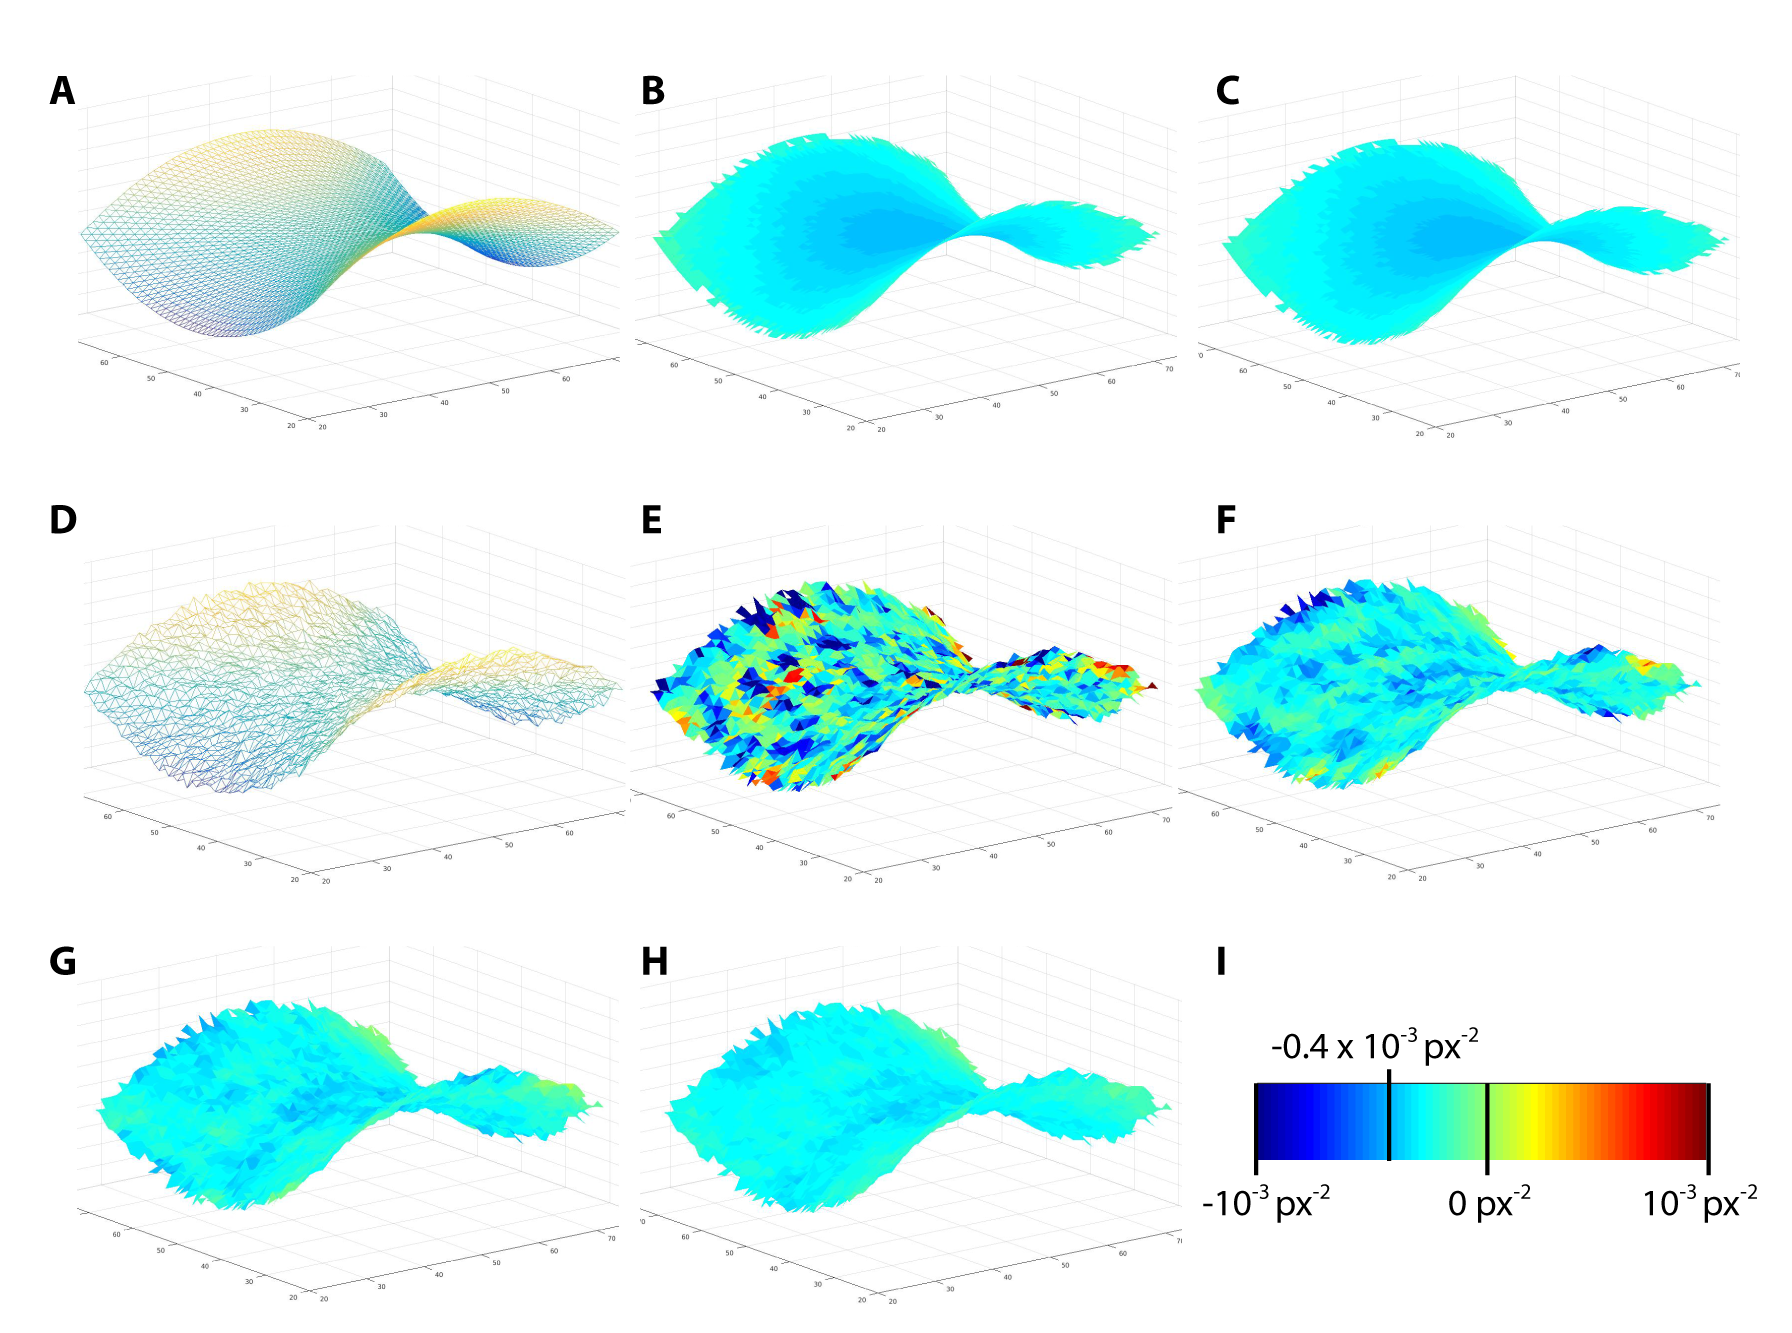
\includegraphics{figures/C3/Ch3-Figs_CurvFitSaddle.png}
  \caption{Fitting the curvature on a saddle surface with varying noise.
  (A-C) A saddle surface with $K = -0.4 \times 10^{-3}$ px$^{-2}$ in the center of the surface.
  The original triangulation is displayed in (A), the output of the initial least-squared fit with $d_1=2$ in (B), and the output of the IRLS fit with $d_2=4$ in (C), with the color scale for the curvature in (I).
  (D-H) The surface in (A) with random noise from a distribution with mean 0 px and width 0.3 px added to the height at every point in the triangulation.
  The triangulation is displayed in (D), the output of the initial least-squared fit with $d_1=4$ in (E), and the output of the IRLS fit with $d_2=6,8,10$ in (F-H), respectively, with the color scale for the curvature in (I).}\label{f:3-CurvFitSaddle}
\end{figure}

We also test a saddle surface with negative Gaussian curvature everywhere on the surface and $K = - 0.4 \times 10^{-3}$ px$^{-2}$ in the middle of the surface.
Similar to the hemisphere, the surface without noise [see Figure~\ref{f:3-CurvFitSaddle}(A)] is insensitive to $d_1$ and $d_2$ [Figure~\ref{f:3-CurvFitSaddle}(B,C), respectively].
In addition, when we fit to a noisy surface [see Figure~\ref{f:3-CurvFitSaddle}(D)], we again see that increasing $d_2$ allows the fit to deal with noise and return Gaussian curvature similar to that of the noiseless surface [Figure~\ref{f:3-CurvFitSaddle}(F--H)].

Overall, our curvature fitting routine works well far from the boundaries.
Near the boundaries, the curvature fit does not always work very well, as seen in the curvature near the corners in Figure~\ref{f:3-CurvFitSphere}(C,F-H), as there is less long-range information available when a point is within $d_2$ of a boundary.
As a consequence, we typically neglect curvature values within $d_2/2$ of the boundary.


\subsection{Measuring the curvature of toroidal droplets}
\begin{figure}
  \centering
  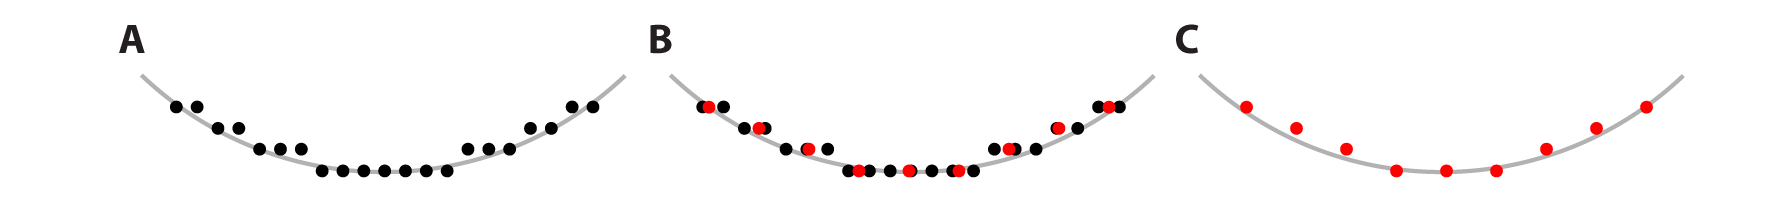
\includegraphics{figures/C3/Ch3-Figs_Sampling.png}
  \caption{Downsampling a surface.
  (A), Imaging the curved contour in gray leads to ``step'' artifacts in the black points.
  (B), We downsample the black points to get the red points.
  (C), The red points still represent the gray contour without so many step artifacts.}\label{f:3-Sampling}
\end{figure}

Before we measure the curvature of the $h(x,y)$ output from time-averaging the intensity of a confocal image stack, we first have to remove measurement artifacts.
Since $h(x,y)$ is a discrete quantity set by the height resolution of the confocal, the triangulated surface appears to have ``steps'' where the measured surface jumps from the height of one image plane to another.
This is illustrated in the schematic in Figure~\ref{f:3-Sampling}(A), where imaging the gray contour leads to steps in the (${\bullet}$) data points.
The steps on the surface are artifacts and affect the curvature measurement; the steps create flat areas with no curvature, while the jumps in height have large curvature.
We remove these steps by downsampling the initial $h(x,y)$ until the output triangulation show no steps.
For our example with the gray contour [Figure~\ref{f:3-Sampling}(A)], we downsample the (${\bullet}$) points, yielding the (${\color{red} \bullet}$) points [Figure~\ref{f:3-Sampling}(B)]; the (${\color{red} \bullet}$) points still represent the gray contour well [Figure~\ref{f:3-Sampling}(C)].
If we downsample too much, we risk eliminating real curvature features in our data.
In practice, we typically downsample $h(x,y)$ with an initial size 512~px~$\times$~512~px to a final size 75~px~$\times$~75~px.
We triangulate the downsampled surface, as shown in Figure~\ref{f:3-CurvFitTorus}(A).
We fit the curvature on the triangulation with $d_1 = 4$ and $d_2 = 12$, as shown in Figure~\ref{f:3-CurvFitTorus}(B,D), and then use linear interpolation to upsample the final $K(x,y)$ and $\sqrt{g}(x,y)$ back to the original size, as seen in Figure~\ref{f:3-CurvFitTorus}(E,F), respectively.
\begin{figure}
  \centering
  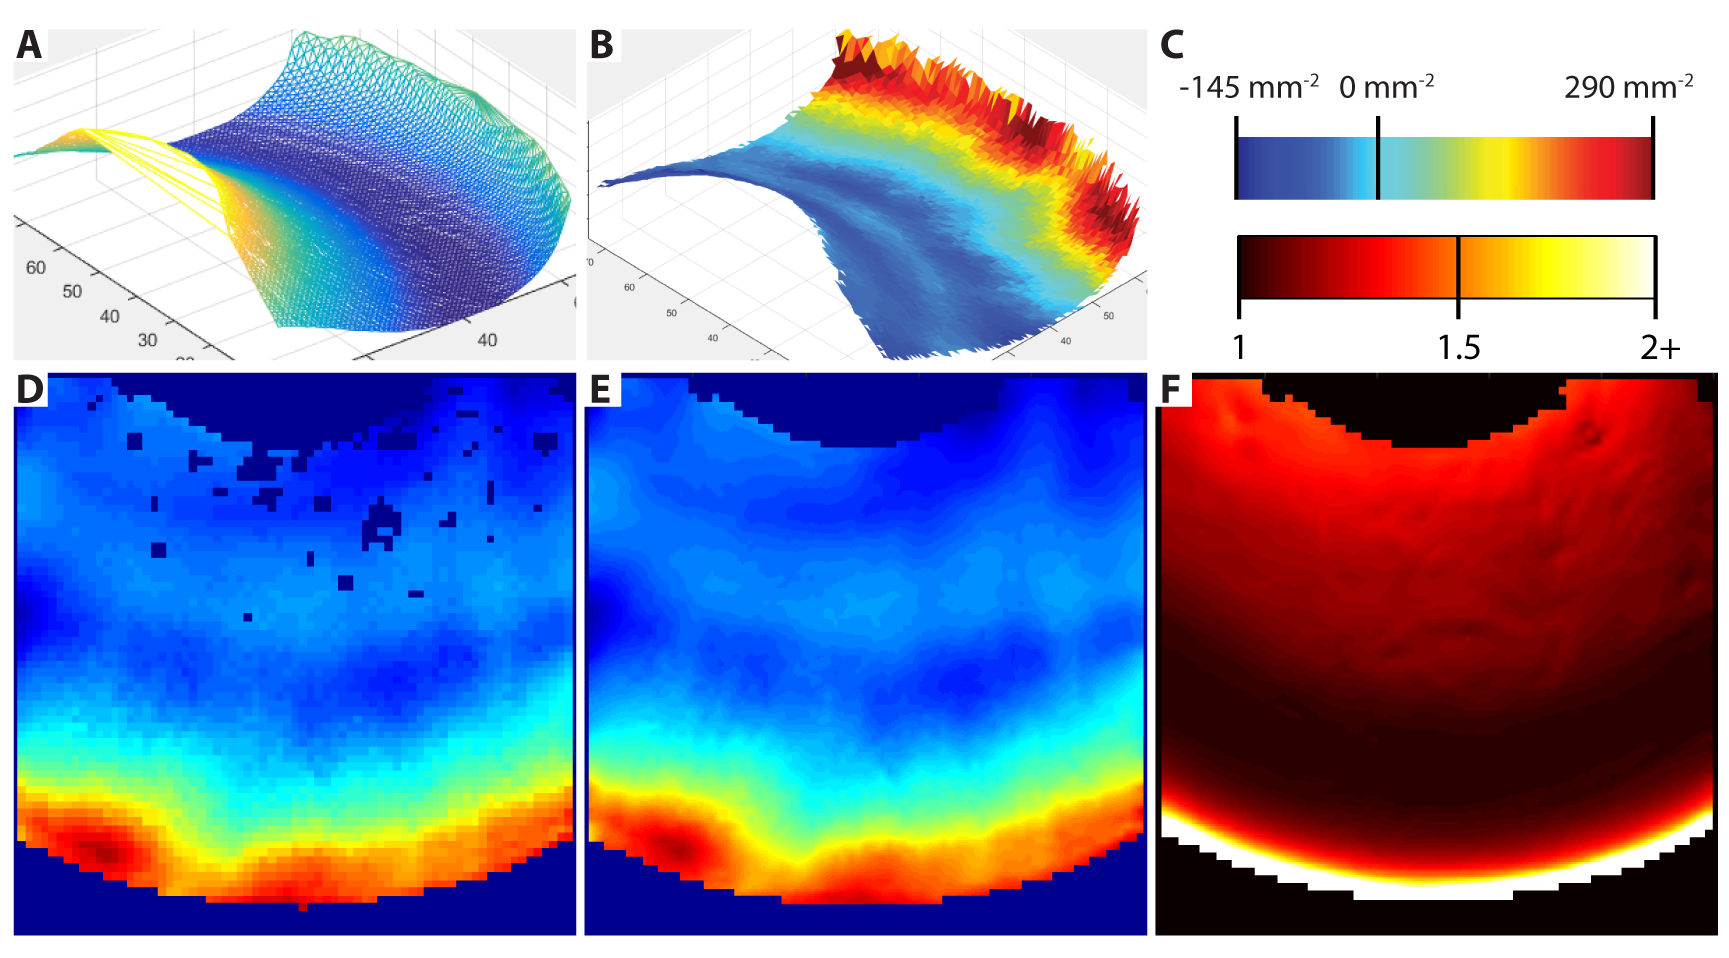
\includegraphics{figures/C3/Ch3-Figs_CurvFitTorus.png}
  \caption{Measuring the Gaussian curvature and $\sqrt{g}$ on a torus.
  (A) Triangulation colored by height formed from a downsampled $h(x,y)$.
  (B-D) The Gaussian curvature of the triangulation in (A) displayed as a (B,D) triangulation and an image, respectively, with the values given by the upper colorbar in (C).
  (E) The Gaussian curvature in (D), upsampled and with missing data filled in using linear interpolation to return the data to its original size.
  (F) The upsampled and filled in $\sqrt{g}$ obtained from the corrected normal vectors with the values given by the lower colorbar in (C).}\label{f:3-CurvFitTorus}
\end{figure}




\section{Defect charge and curvature}
From the fitted curvatures and the defect locations over time, we look to compare the time-averaged topological charge in a region with the integrated Gaussian curvature of the region.


\subsection{Finding regions of specific integrated Gaussian curvature}
We start by considering a binary mask $\Theta_0(x,y)$ representing the full area in the intensity projection where we have data for the director field.
We then remove the outer 10~px to 30~px of $\Theta_0(x,y)$ by successively finding the boundary $\partial \Theta_0$ of the region and setting the pixels to $0$ until $\Theta_0(x,y)$ only contains places where we trust the curvature.
This mask serves as our base from which we will determine any subregion $\Theta(x,y)$ we wish to look at.
From some $\Theta(x,y)$, we calculate the integrated Gaussian curvature in that region numerically,
\begin{equation}
  \oint_{\Theta}\,K\textrm{dA} \approx \sum\limits_{x,y} \Theta(x,y) K(x,y) \sqrt{g}(x,y).
\end{equation}
Since the area is positive-definite, the maximum integrated Gaussian curvature and the minimum integrated Gaussian curvature masks are easy to generate simply by starting with the base $\Theta_0(x,y)$ and setting the pixels with $K < 0$ or $K > 0$ to $0$.
These two masks define the range of integrated Gaussian curvature that we can probe for the imaged section of a single toroid.
We can also easily divide the base $\Theta_0(x,y)$ into halves or thirds to consider regions of different integrated Gaussian curvature.

We can also find regions with specific values of integrated Gaussian curvature.
From some starting $\Theta(x,y)$ we calculate the starting integrated Gaussian curvature and determine whether it is greater or less than the desired value.
The routine then finds the boundary, $\partial \Theta$, and sets all the pixels on $\partial \Theta$ with the appropriately signed $K$ to $0$.
For example, if the current integrated Gaussian curvature is greater than the target integrated Gaussian curvature, all the boundary pixels with $K > 0$ are set to $0$.
This process is repeated until the difference between the current integrated Gaussian curvature and the target integrated Gaussian curvature changes sign.
The routine then takes the most recently removed boundary pixels and adds them back to the modified $\Theta(x,y)$ one-by-one until the difference between the current integrated Gaussian curvature and the target integrated Gaussian curvature has the same sign as the difference between the initial integrated Gaussian curvature and the target integrated Gaussian curvature.


\subsection{Time-averaged defect charge as a function of integrated Gaussian curvature: curvature-induced defect unbinding}
We correlate the time-averaged topological charge in a region with the integrated Gaussian curvature of that region for both 36~mM ATP and 144~mM ATP.
We find that for both ATP concentrations, $\overbar{s}_{\Theta}$ is linear with $\int_{\Theta}\,K\textrm{dA}$, a shown in Figure~\ref{f:3-DefectUnbinding}, where we plot data from toroids with a range of $\xi$ and $a$.
The slope of each curve, $C'$, is positive, consistent with the curvature-induced defect unbinding predicted theoretically.
Recall that for an equilibrium nematic, we expect the charge to be a discrete multiple of $1/2$ and increases as a step function as we integrate $K$ along the azimuthal direction [see Figure~\ref{f:3-EqDefs}(A)].
However, due to the large number of defects and their constant motion, the time-averaged topological charge becomes a real number.
Furthermore, $\overbar{s}_{\Theta}$ only depends on the integrated Gaussian curvature and is independent of $\xi$ and $a$.
This implies that the unbinding only depends on the local geometry and is insensitive to the  global size and shape of the system.

This in direct contrast to equilibrium simulations and theory, where defect unbinding only appears in toroids with curvatures large enough to overcome the attraction between opposite signed defects~\cite{RN36,RN22}.
In addition, in equilibrium systems, the repulsions between like-signed defects and the defect core energies affect the number of defects in a defective ground state~\cite{RN36}.
This implies that in equilibrium, $\xi$ and $a$ are predicted to not only affect whether or not defects exist in the ground state, but also the number of defects in the ground state~\cite{RN36,RN19,RN22,RN20,RN78}.

We also note that the lines in Figure~\ref{f:3-DefectUnbinding}(A,B) both go through $(0,0)$, indicating that regions with $\oint_{\Theta}\,K\textrm{dA} = 0$ have $\overbar{s}_{\Theta} = 0$, a topological requirement for the entire toroid.
In our case, however, we see that this is true irrespective of the region we consider, provided the region has vanishing integrated Gaussian curvature.
This is shown explicitly in Figure~\ref{f:3-ChargeOverTime}, where all the regions under consideration, Figure~\ref{f:3-ChargeOverTime}(A,C,E), have $\int_{\Theta}\,K\textrm{dA} = 0$ and vanishing time-averaged topological charge [Figure~\ref{f:3-ChargeOverTime}(B,D,F)].
This implies that a region with $\oint_{\Theta}\,K\textrm{dA} = 0$ is representative of an entire toroid.
Again, this is in contrast to equilibrium nematics, where the small defect number and lack of significant defect motion result in different regions with the same net integrated Gaussian curvature generally enclosing a different topological charge.
Finally, we see that changing the ATP concentration yields a different amount of unbinding, with $C' = 4.3 \pm 0.7$ for the 144 $\upmu$M ATP concentation and $C' = 6.3 \pm 0.5$ for the 36 $\upmu$M ATP concentration, indicating that increasing activity leads to less curvature-induced unbinding.
This is seen explicitly in Figure~\ref{f:3-DefectUnbinding}(C), where we plot the data for both ATP concentrations to emphasize that ATP and thus activity is the dominant factor in the amount of unbinding.
\begin{figure}
  \centering
  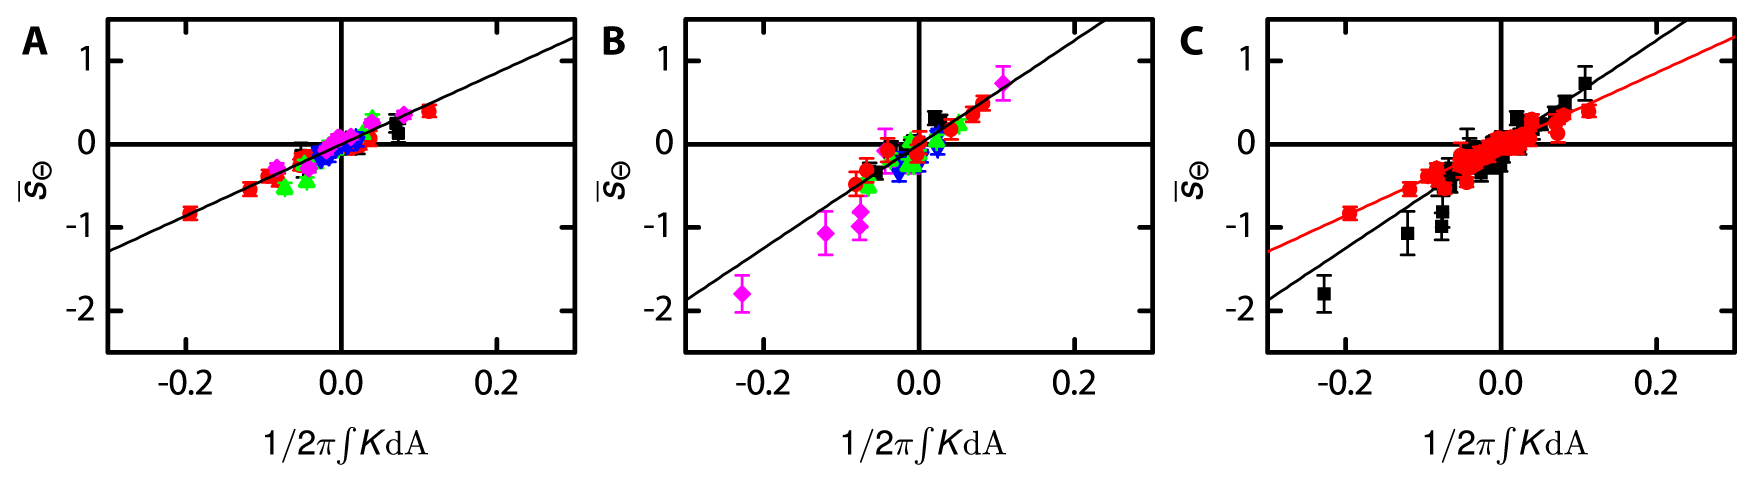
\includegraphics{figures/C3/Ch3-Figs_DefectUnbinding.png}
  \caption{Defect unbinding in active nematic toroids.
  (A,B) Time-averaged topological charge in an area vs the integrated Gaussian curvature of the area for toroids with (A) 144 $\upmu$M ATP, (B) 36 $\upmu$M ATP, and (C) both ATP concentrations with the data from (A) in red and the data from (B) in black.
  The lines in (A) and (B) are weighted averages of a linear fit to the data for each individual toroid in the plot and have slopes $4.3 \pm 0.7$ and $6.3 \pm 0.5$, respectively with intercepts $0.01 \pm 0.02$ and $0.02 \pm 0.03$, respectively.
  The toroids in (A) have:
  $({\color{red} \bullet})$ $\xi = 1.6 $ and $a = 275$ $\upmu$m,
  $({\color{green} \blacktriangle})$ $\xi = 2.0 $ and $a = 372$ $\upmu$m,
  $({\color{magenta} \blacklozenge})$ $\xi = 2.4 $ and $a = 268$ $\upmu$m,
  $({\blacksquare})$ $\xi = 5.9$ and $a = 200$ $\upmu$m, and
  $({\color{blue} \blacktriangledown})$ $\xi = 6.6$ and $a = 167$ $\upmu$m.
  The toroids in (B) have:
  $({\color{red} \bullet})$ $\xi = 1.8 $ and $a = 334$ $\upmu$m,
  $({\color{green} \blacktriangle})$ $\xi = 2.7 $ and $a = 365$ $\upmu$m,
  $({\color{magenta} \blacklozenge})$ $\xi = 3.6 $ and $a = 151$ $\upmu$m,
  $({\blacksquare})$ $\xi = 4.7$ and $a = 200$ $\upmu$m, and
  $({\color{blue} \blacktriangledown})$ $\xi = 6.0$ and $a = 547$ $\upmu$m.}\label{f:3-DefectUnbinding}
\end{figure}

Thus, our results suggest that activity is playing a role that reminds us of temperature in equilibrium systems.
In 2D, the  nematic-isotropic phase transition is predicted to be continuous~\cite{RN172}, such that the nematic elasticity should vanish smoothly on the approach to the phase transition.
As an equilibrium nematic gets sufficiently close to the nematic-isotropic phase transition, thermal fluctuations will begin to play an increasingly dominant role.
The fluctuations will eventually mobilize the defects and produce results that could resemble in some ways what we see in our active nematic.




\section{Defect number distributions}
Because of the continuous creation, annihilation, and motion of the defects, the defect number in a region fluctuates over time, as shown in Figure~\ref{f:3-NumberOverTime}(B).
For the 144~$\upmu$M ATP toroids, we have enough timeframes to obtain the defect number distribution for regions containing different $\overbar{N}_{\Theta}$.
The defect number distributions are Gaussian, as shown in Figure~\ref{f:3-ExpDistribution}(B,D,F) for three distributions obtained on the same toroid with $\xi = 1.6$ and $a = 275$ $\upmu$m; each distribution is obtained from the region bounded with the white border in the associated image in Figure~\ref{f:3-ExpDistribution}(A,C,E), respectively.
In each image, the region is not necessarily contiguous and has vanishing integrated Gaussian curvature; however, each region has a different total area [see Figure~\ref{f:3-ExpDistribution}(A,C,E)].

Since the data are described by a Gaussian, we obtain both the fluctuations in the defect number, $\displaystyle{\sqrt{\Delta N_{\Theta}^2}}$, and the mean number of defects, $\overbar{N_{\Theta}}$, by fitting each distribution to $A \exp (-\overbar{N_{\Theta}}^2/(2 \Delta N_{\Theta}^2))$, with $A$ a free parameter [see Figure~\ref{f:3-ExpDistribution}(B,D,F)].
We then plot the relative root-mean-squared (RMS) fluctuations, $\displaystyle{\sqrt{\Delta N_{\Theta}^2}} \bigg / \displaystyle {\overbar{N}_{\Theta}}$, vs $\overbar{N}_{\Theta}$ for every region on all of our toroids on a log-log plot, as shown in Figure~\ref{f:3-ExpDistribution}(G).

We see that like the time-averaged topological charge, all the data collapse onto a line, regardless of the $\xi$ and $a$ variation between the toroids.
We take the weighted average of a linear fit on a log-log scale to the data from each individual toroid, where the error in the fit determines the weight, and find a final slope $-0.53 \pm 0.04$ and final intercept $0.02 \pm 0.04$.
This means that $\displaystyle{\sqrt{\Delta N_{\Theta}^2}} \bigg / \displaystyle {\overbar{N}_{\Theta}} \sim \overbar{N}_{\Theta}^{-1/2}$, which is the expected result for an equilibrium system subject to number fluctuations~\cite{RN311, gaussianApprox}.
Again, this suggests that the role of activity is somewhat reminiscent to the role of temperature in equilibrium systems.
\begin{figure}
  \centering
  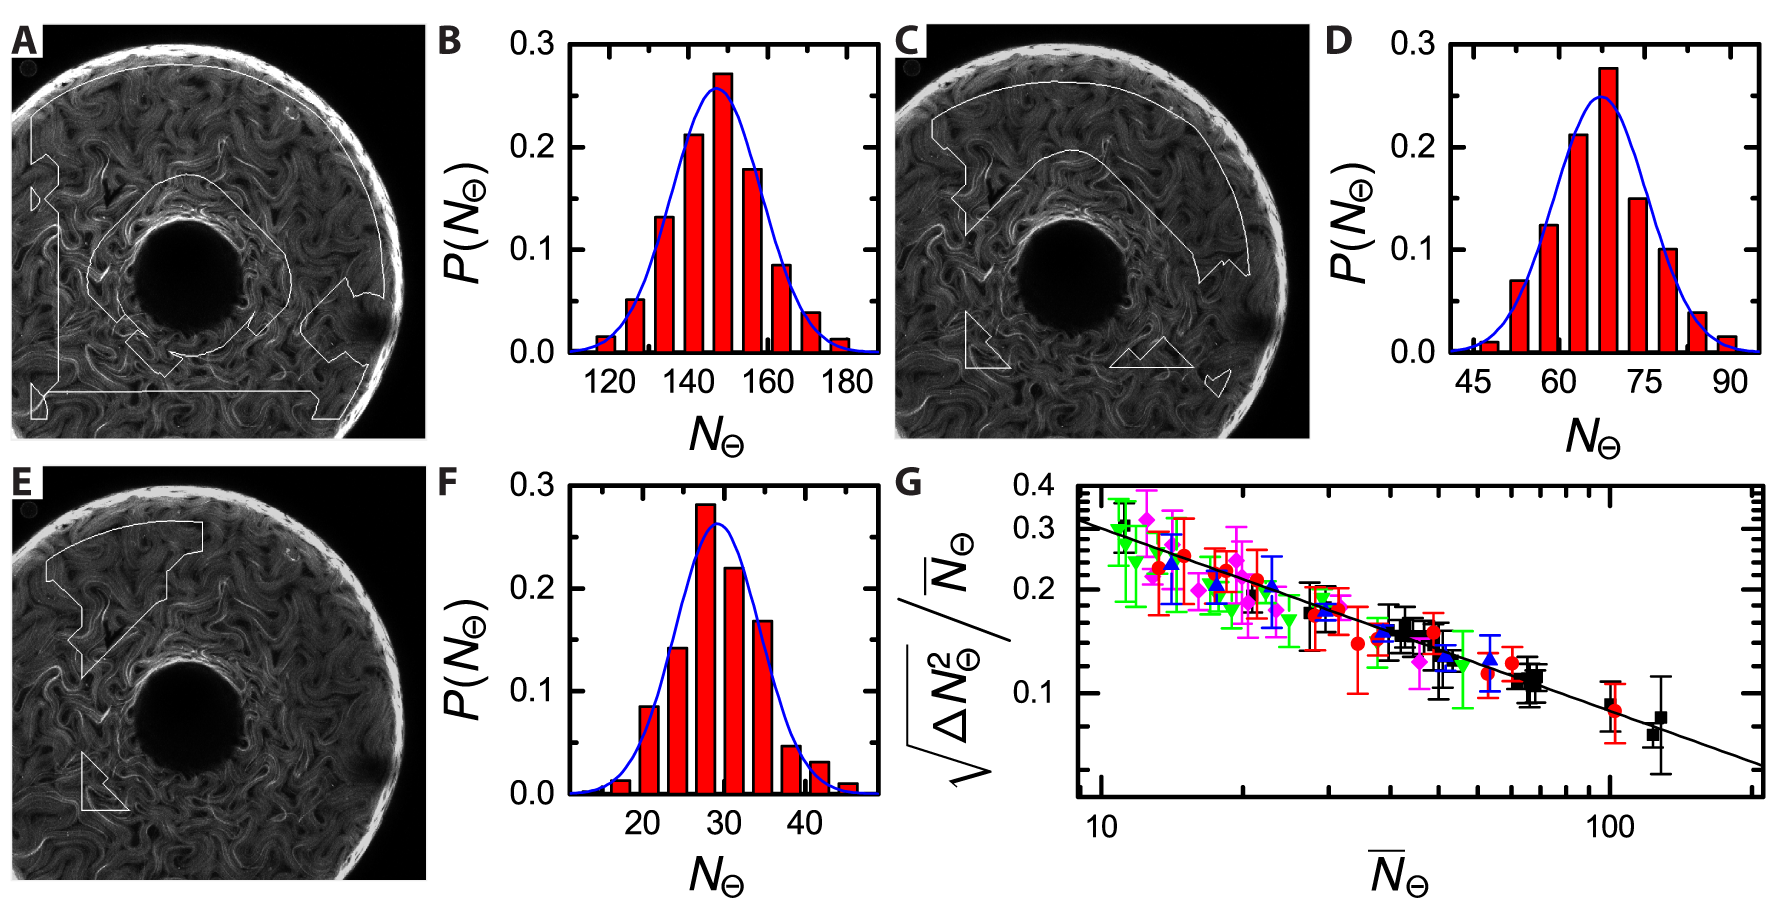
\includegraphics{figures/C3/Ch3-Figs_ExpDistribution.png}
  \caption{Defect number distributions.
  (A,C,E) For an experiment with $\xi = 1.6$ and $a = 275$ $\upmu$m, the regions outlined in white have vanishing integrated Gaussian curvature and total area (A) $A_{\Theta} = 0.75$ mm$^{-2}$, (B) $A_{\Theta} = 0.34$ mm$^{-2}$, and (C) $A_{\Theta} = 0.15$ mm$^{-2}$.
  (B,D,F) The probability of finding a number of defects in the regions in (A,C,E), respectively.
  (G) The relative RMS defect number fluctuations in a region vs the time-averaged defect number in the region for experiments with
  $({\blacksquare})$ $\xi = 1.6 $ and $a = 275$ $\upmu$m,
  $({\color{red} \bullet})$ $\xi = 2.0 $ and $a = 372$ $\upmu$m,
  $({\color{green} \blacktriangle})$ $\xi = 2.4 $ and $a = 268$ $\upmu$m,
  $({\color{blue} \blacktriangledown})$ $\xi = 5.9$ and $a = 200$ $\upmu$m, and
  $({\color{magenta} \blacklozenge})$ $\xi = 6.6$ and $a = 167$ $\upmu$m.
  The line is the weighted average of a linear fit on a log-log scale to the data for each individual toroid and has slope $-0.53 \pm 0.04$ and intercept $0.02 \pm 0.04$.}\label{f:3-ExpDistribution}
\end{figure}



\section{Comparison with numerical simulations}
To gain further insight about our experimental findings, we compare with numerical simulations performed by Luca Giomi and Dan Pearce at the University of Leiden.
The simulations treat the defects as point particles with the system energy given by Eq.~\ref{e:1-TopTheoryofDefects}.
For a torus with $N$ defects, the simulation has $N/2$ $s = +1/2$ defects and $N/2$ $s = -1/2$ defects in order to satisfy the Poincar\'e-Hopf Theorem.


\subsection{Simulation details}
Defects are modeled as massless particles on the torus [see Figure~\ref{f:3-SimDefectUnbinding}(A)], with the $i^{\rm th}$ defect having charge $s_{(i)}$, position $\mathbf{r}_{(i)}$, and orientation $\mathbf{p}_{(i)} = -\cos \psi \, \hat{\theta} + \sin \psi \, \hat{\varphi}$, with $\hat{\theta}$ and $\hat{\varphi}$ unit vectors on the surface of the torus [Figure~\ref{f:3-EqDefs}], and $\psi$ an angle in the tangent plane measured off of $\hat{\theta}$.
The defects are governed by the following equations of motion,
\begin{align}
  \frac{\textrm{d}\mathbf{r}_{(i)}}{\textrm{d}t} &= v_0 \mathbf{p}_{(i)} + \mu \Big [\sum\limits_{j\neq i=1}^N \mathbf{F}_{(ij)} - \nabla_{(i)} V \Big ] + \bm{\zeta}^{trans}_{(i)} \\
    \frac{\textrm{d}\psi_{(i)}}{\textrm{d}t} &= \zeta^{rot}_{(i)},
\end{align}
where $v_0$ is the speed associated to the self-propulsion of the $s = +1/2$ defects, $\mu$ is a mobility coefficient, and $\bm{\zeta}^{trans}_{(i)}$ and $\zeta^{rot}_{(i)}$ are uncorrelated translational and rotational noises, reproducing the fluctuations of the defects\cite{uncorrelatedNoise}.
Both $\mathbf{F}_{(ij)}$ and $V_{(i)}$ are calculated from Eq.~\ref{e:1-TopTheoryofDefects},
\begin{align}
  \mathbf{F}_{(ij)} &= 4\pi^2 k_F s_{(i)}s_{(j)} \nabla_{(j)} G(\mathbf{r}_{(i)},\mathbf{r}_{(j)})\label{e:defectdefectforce} \\
  V &= - 2 \pi s_{(i)}k_F \int \textrm{d}A\, G(\mathbf{r},\mathbf{r}_{(i)})K(\mathbf{r}),\label{e:defectsurfaceenergy}
\end{align}
where $G(\mathbf{r}_{(i)},\mathbf{r}_{(j)})$ is the Laplacian Green function on the torus and $k_F$ is the Frank constant in 2D.
$\mathbf{F}_{(ij)}$ and $V_{(i)}$ are, respectively, the force resulting from defect-defect interactions and the potential energy associated to the interaction between the defect and the local Gaussian curvature.

There are three main material parameters in an active nematic that affect its dynamics, $\alpha$, $k_F$, and the shear viscosity, $\eta$.
Since the simulations are in 2D, these quantities are all 2D and have units $[\alpha] = {\rm Force}/{\rm Length}$, $[k_F] = {\rm Force} \times {\rm Length}$, and $[\eta] = {\rm Force} \times {\rm Time} / {\rm Length}$.
From Eq.~\ref{e:3-NavierStokes} we know that $\alpha$ measures the strength of the activity that causes the nematic to deform.
Since these deformations are resisted by the passive nematic elasticity, we can combine $\alpha$ and $k_F$ to form the active length scale $\ell_a = \sqrt{k_F / |\alpha|}$, that represents the length at which the active stresses and passive elastic stresses balance.
The active stress can deform the material when the wavelength of the distortion is longer than $\ell_a$, but the passive elasticity prevents deformations with a shorter wavelength.
In this sense, $\ell_a$ can be thought of as the buckling length of the active nematic, giving the size of the distortion surrounding a $s = \pm 1/2$ defect.
Thus, when $\ell_a \lesssim L$, with $L$ the system size, the passive elasticity and the active stresses roughly balance and few defects are created~\cite{RN7}.
In this regime, the flow is laminar~\cite{RN7}.
However, when $\ell_a \ll L$, the active stresses dominate and pairs of $s = \pm 1/2$ spontaneously create and annihilate.
The passive elasticity prevents like-signed defects from having a separation distance smaller than $\ell_a$; similarly, the active stresses create a $s = \pm 1/2$ defect pair whenever there is a region of undistorted nematic larger than $\ell_a$~\cite{RN7}.
As a consequence, the active length scale is proportional to and of the same order of magnitude as the distance between defects, $\lambda = \sqrt{A_{torus}/N} = 2 \pi a \sqrt{\xi/N}$, with $A_{torus} = 4 \pi^2 R_0 a = 4 \pi^2 \xi a^2$, the surface area of a torus.

Due to the large number of defects and their constant motion, the nematic dynamics become turbulent, with the characteristic velocity of the $s = +1/2$ defects as $v_0 \approx \alpha \ell_a/ \eta = \textrm{sign}(\alpha) \sqrt{|\alpha| k_F}/\eta$.~\cite{RN7, turbulentNematic}.
Thus, the dimensionless distance between defects $\lambda' = \lambda/a$ and the dimensionless speed $v_0' = v_0 a /(\mu k_F)$ specify all the relevant material properties of the active nematic in the numerical simulations.
\begin{figure}
  \centering
  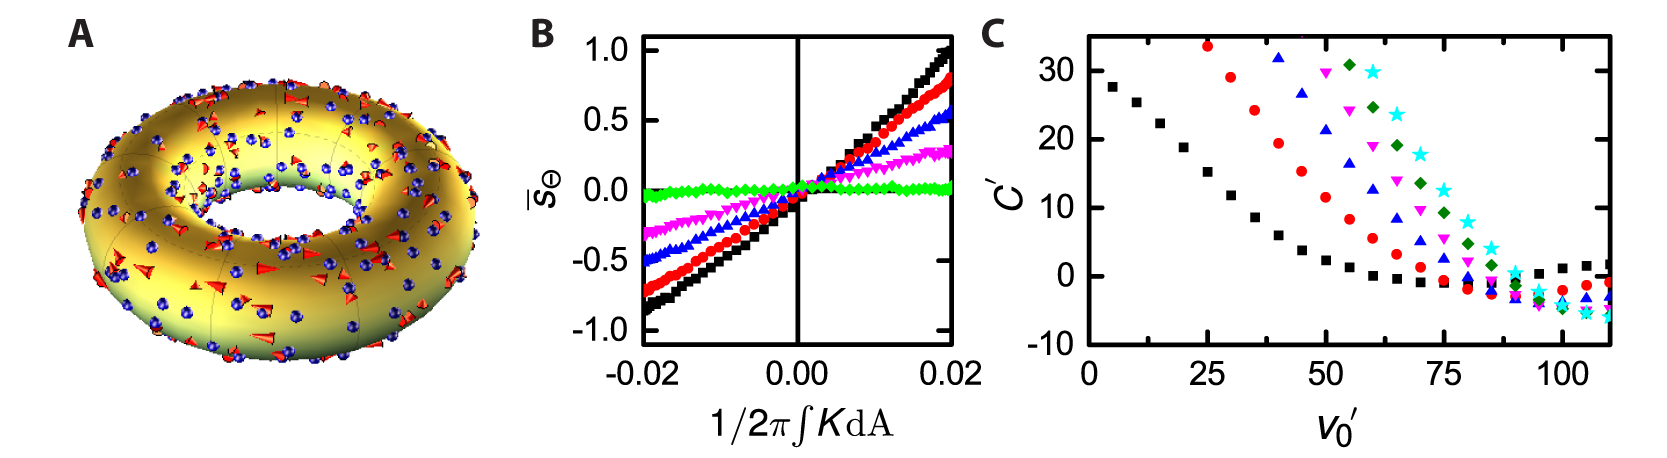
\includegraphics{figures/C3/Ch3-Figs_SimDefectUnbinding.png}
  \caption{Defect unbinding in simulations depends on defect velocity and defect density.
  (A) Schematic of a torus with $\xi = 3$ and 250 defect pairs on the surface ($\lambda' = 0.49$) at a single moment in time.
  (B), Plot of time-averaged topological charge in a region vs the integrated Gaussian curvature  in that region for a simulation with $\lambda' = 0.49$ and
  $({\blacksquare})$ $v'_0 = 10$,
  $({\color{red} \bullet})$ $v'_0 = 20$,
  $({\color{blue} \blacktriangle})$ $v'_0 = 30$,
  $({\color{magenta} \blacktriangledown})$ $v'_0 = 40$, and
  $({\color{green} \blacklozenge})$ $v'_0 = 60$.
  (C) The slope of the curves in (B), $C'$, vs defect velocity for simulations with
  $({\blacksquare})$ $\lambda' = 0.69$,
  $({\color{red} \bullet})$ $\lambda' = 0.49$,
  $({\color{blue} \blacktriangle})$ $\lambda' = 0.40$,
  $({\color{magenta} \blacktriangledown})$ $\lambda' = 0.34$,
  $({\color{green} \blacklozenge})$ $\lambda' = 0.31$, and
  $({\color{teal} \star})$ $\lambda' = 0.28$.}\label{f:3-SimDefectUnbinding}
\end{figure}

For fixed $\lambda'$, we find that $\overbar{s}_{\Theta}$ is a linear function of the integrated Gaussian curvature, and the line passes through $(0,0)$.
This implies that, as in the experiments, regions with vanishing integrated Gaussian curvature are representative of the full torus.
However, in the simulation, we can easily tune $v'_0$.
For increasing $v'_0$, we find that $C'$ decreases [see Figure~\ref{f:3-SimDefectUnbinding}(B)], eventually approaching zero.
At this point, activity dominates over the elastic forces associated to defect-curvature interactions, confirming that, from this perspective, the role of activity is reminiscent of the expected role of thermal fluctuations close to the nematic-isotropic phase transition in passive nematics.
However, we emphasize that in equilibrium, both the $s = +1/2$ and the $s = -1/2$ defects would randomly explore the toroid as a result of thermal motion.
This is in contrast to our active system, where only the $s = +1/2$ defects are driven by activity.
In addition, the direction of the velocity of an $s = +1/2$ defect is determined by the defect's structure, while in passive nematics thermal fluctuations will cause the defect to diffuse isotropically.
The motion of the $s = +1/2$ defects can thus be thought of as a persistent, or correlated, random walk, where the defect's current trajectory influences its future trajectory.
Finally, we see that the observed behavior of $C'$ with $v'_0$ is maintained irrespective of $\lambda'$, as shown in Figure~\ref{f:3-SimDefectUnbinding}(C).


\subsection{Matching simulation parameters to experiment}
To quantitatively compare the experimental and simulated results, we need $\lambda'$ and thus the total defect density on our experimental toroids.
Since both our simulations and our experiments indicate that regions with vanishing integrated Gaussian curvature are representative of the full torus, that is, that $\overbar{N}/A_{torus} = \overbar{N}_{\Theta}/A_{\Theta}$, where  $\int_{\Theta} K\, \textrm{d}A = 0$, we use these regions to compare between the experiment and the simulation.
We note that $\overbar{N}_{\Theta}/A_{\Theta}$ varies linearly with $\langle K \rangle_{\Theta} = (\int_{\Theta}K\,\textrm{d}A)/A_{\Theta}$ such that we can fit a line to this relation and take the value of $\overbar{N}_{\Theta}/A_{\Theta}$ at $\langle K \rangle_{\Theta} = 0$ to be $\overbar{N}/A_{torus}$ [see Figure~\ref{f:3-MatchParam}].
We calculate $\lambda'$ for each toroid and find that the $\lambda'$ values for each ATP concentration are similar to each other.
Thus, we take a weighted average to obtain $\lambda' = 0.31 \pm 0.04$ and $\lambda' = 0.3 \pm 0.1$ for the 144 $\upmu$M and 36 $\upmu$M ATP concentrations, respectively.
In addition, we perform a weighted average on the value of $\overbar{N}_{\Theta}/A_{\Theta}$ for $\langle K \rangle_{\Theta} = 0$ to get the defect density for each ATP concentration, with $\overbar{N}/A_{torus} = (157 \pm 19)$ defects/mm$^{2}$ for the for the 144 $\upmu$M ATP concentration and $\overbar{N}/A_{torus} = (90 \pm 14)$ defects/mm$^{2}$ for the 36 $\upmu$M ATP concentration.
We see that in our experiments, increasing $|\alpha|$ leads to increasing values of $\overbar{N}/A_{torus}$, consistent with the idea that $\ell_a = \sqrt{k_F / |\alpha|} \sim \lambda = \sqrt{A_{torus}/\overbar{N}}$.
However, $\lambda'$ doesn't change between the ATP concentrations in our experiments because the toroids we used for the 36 $\upmu$M ATP concentration had a larger tube radius than the toroids used for the experiments with 144 $\upmu$M ATP.
\begin{figure}
  \centering
  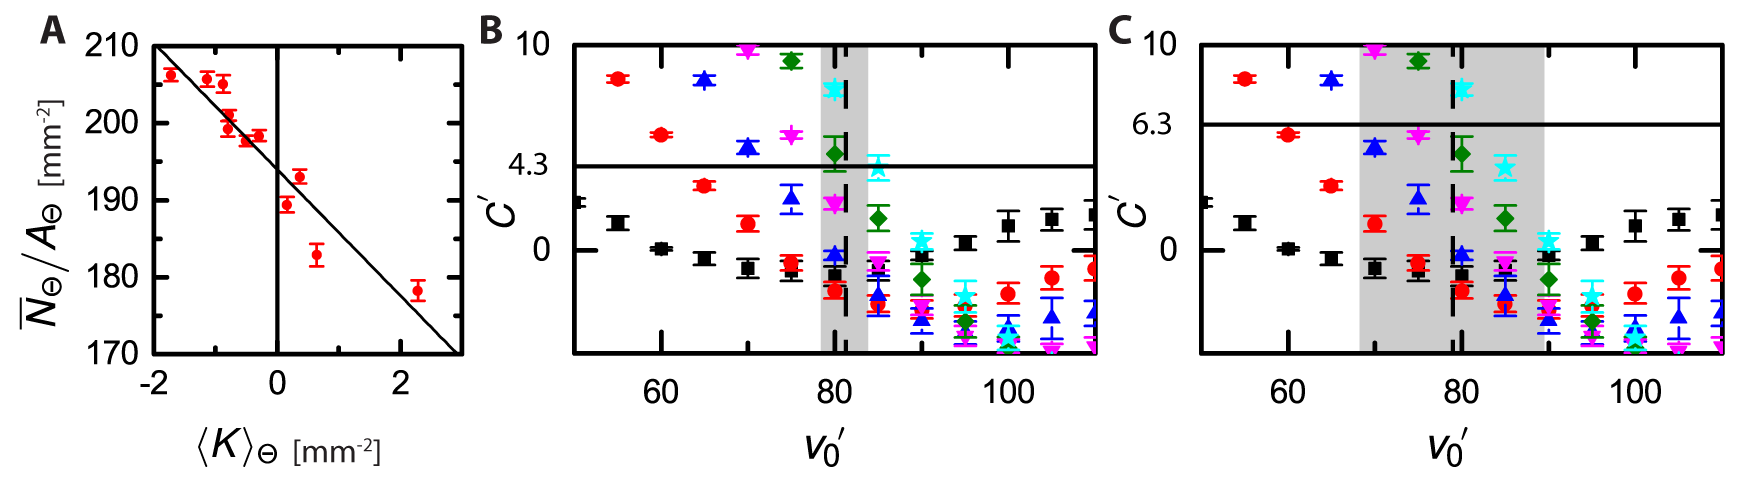
\includegraphics{figures/C3/Ch3-Figs_MatchParam.png}
  \caption{Quantitatively comparing experiment and simulation.
  (A) Time-averaged defect density in a region vs the mean Gaussian curvature of that region for an experiment with $\xi = 1.6$, $a = 275$ $\upmu$m.
  (B,C) $C'$ vs defect velocity for simulations with
  $({\blacksquare})$ $\lambda' = 0.69$,
  $({\color{red} \bullet})$ $\lambda' = 0.49$,
  $({\color{blue} \blacktriangle})$ $\lambda' = 0.40$,
  $({\color{magenta} \blacktriangledown})$ $\lambda' = 0.34$,
  $({\color{green} \blacklozenge})$ $\lambda' = 0.31$, and
  $({\color{teal} \star})$ $\lambda' = 0.28$,
  with the horizontal line corresponding to the experimental value of (B) $C' = 4.3$ for the 144 $\upmu$M ATP toroids and (C) $C' = 6.3$ for the 36 $\upmu$M ATP toroids.
  In both plots, the vertical dashed line marks the crossing of the horizontal line and the $\lambda' = 0.31$ simulation curve, with the gray background giving the error due to the uncertainty in the $\lambda'$ for the respective experimental measurements.}\label{f:3-MatchParam}
\end{figure}

We now return to the plot of $C'$ vs $v'_0$ and indicate our experimentally measured $C'$ values with a horizontal line, as seen in Figure~\ref{f:3-MatchParam}(B,C) for 144 $\upmu$M and 36 $\upmu$M ATP, respectively.
We then consider our experimental values of $\lambda'$  and highlight the crossing point between the experimentally measured $C'$ values and the relevant simulation curve with a vertical dashed line.
This crossing point gives the values $v'_0 = 81 \pm 2$ and $v'_0 = 80 \pm 10$, for the 144 $\upmu$M and 36 $\upmu$M ATP concentration.
Rewriting the expression for $v'_0$ in terms of $\lambda'$, we have $v'_0 = (|\alpha|a^2 \lambda')/(\mu \, k_F \, \eta)$, showing that the large uncertainty in $v'_0$ for the 36 $\upmu$M ATP toroids comes from the large uncertainty in the associated $\lambda'$.
However, since we see that $v'_0$ doesn't change appreciably when we change $\alpha$ in our experiments, this implies that one or more of $\mu$, $k_F$, and $\eta$ must also depend on $\alpha$.

We confirm our estimate of $v'_0$ for the 144 $\upmu$M ATP concentration by calculating the defect number distributions in the simulations.
Similar to the experiment, we see that the probability of finding a number of defects in a region is Gaussian [see Figure~\ref{f:3-MatchDist}(A)].
In the simulation, however, we have the ability to easily vary $v'_0$.
We plot $\displaystyle{\sqrt{\Delta N_{\Theta}^2}} \bigg / \displaystyle {\overbar{N}_{\Theta}}$ vs $\overbar{N}_{\Theta}^{-1/2}$ and see they are linearly related, as shown for 3 values of $v'_0$ in Figure~\ref{f:3-MatchDist}(B).
We then correlate $\displaystyle \sqrt{\Delta N_{\Theta}^2 \big / \overbar{N}_{\Theta}}$ with $v'_0$ and plot the relationship in Figure~\ref{f:3-MatchDist}(C), where the vertical line corresponds to the experimental result of $v'_0 = 81 \pm 2$.
Comparing with the simulation, we find $\displaystyle \sqrt{\Delta N_{\Theta}^2 \big / \overbar{N}_{\Theta}} \approx 0.99$, shown with a dashed line in Figure~\ref{f:3-MatchDist}(C).
From the intercept of the line plotted in Figure~\ref{f:3-ExpDistribution}(G), we obtain $\displaystyle \sqrt{\Delta N_{\Theta}^2 \big / \overbar{N}_{\Theta}} = 1.02 \pm 0.04$, consistent with the numerical results.
\begin{figure}
  \centering
  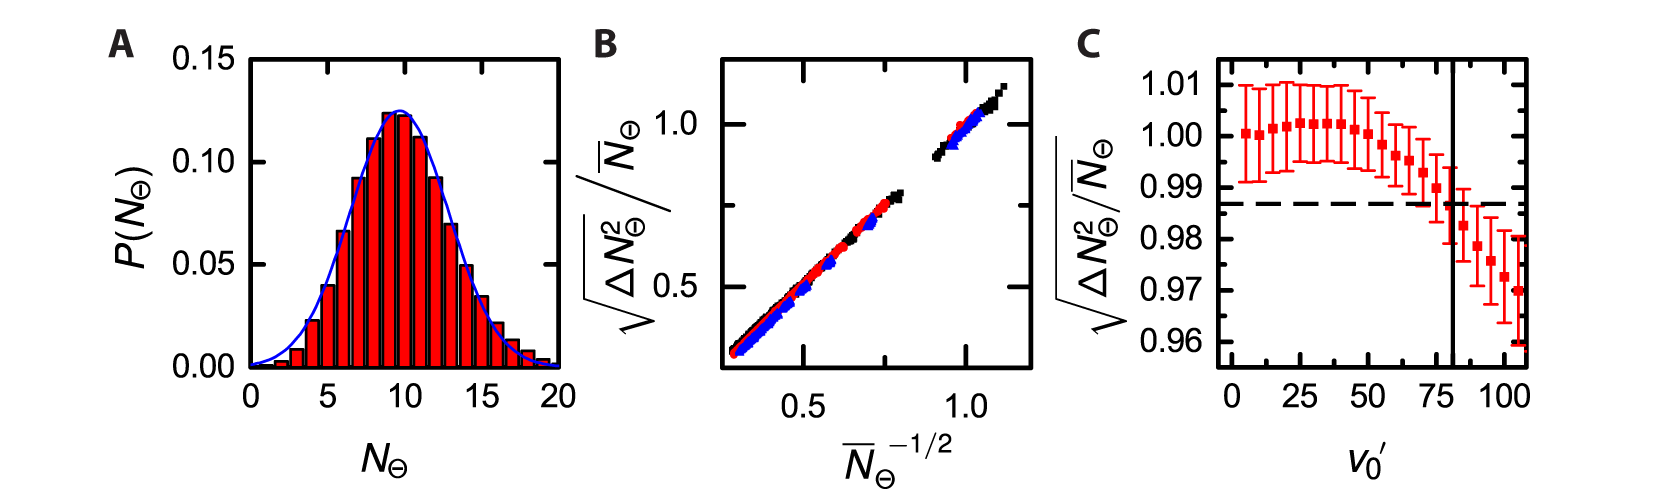
\includegraphics{figures/C3/Ch3-Figs_MatchDist.png}
  \caption{Defect number fluctuations depend on defect velocity.
  (A) Probability of finding a number of defects in a given region for a simulation with $\lambda' = 0.49$, $v'_0 = 50$. The blue curve is a fit of the data to a Gaussian.
  (B) Relative RMS defect number fluctuations in a region vs $\overbar{N}_{\Theta}^{-1/2}$, with $\overbar{N}_{\Theta}$ the time-averaged number of defects in the region for simulations with
  $({\blacksquare})$ $v'_0 = 4$,
  $({\color{red} \bullet})$ $v'_0 = 50$, and
  $({\color{blue} \blacktriangle})$ $v'_0 = 80$.
  (C) Slope of the relative RMS fluctuations vs $\overbar{N}_{\Theta}^{-1/2}$ plotted against the dimensionless defect velocity. The vertical solid line corresponds to $v'_0 = 81$.}\label{f:3-MatchDist}
\end{figure}

The agreement between the experiments and the theory reveals that the interaction between curvature and topological charge depends only on two parameters: (i) the dimensionless mean distance between defects, $\lambda'$, and (ii) the dimensionless speed of the defects, $v_0'$, which relates to the intrinsic activity of the system.
We emphasize that both of these parameters reflect local interactions that do not depend on the global size or geometry of the system.
We find that because of the large number of defects and their constant motion, the average topological charge becomes a continuous variable.
In addition, our results confirm that that in the turbulent regime and free of any influence by a boundary, the mean distance between defects acts as a
proxy for $\ell_a$.
Finally, in our experiments, we managed to change $\alpha$ while keeping $\lambda'$ constant.
Since $v_0'$ also doesn't change when we change $\alpha$, we see that one or more of $\mu$, $k_F$, and $\eta$ must also depend on $\alpha$.


\subsection{Estimates of material parameters}
The agreement between the experiment and the theory prompts us to use the topological defects as micro-rheological tracers and perform “topological micro-rheology” to estimate the material parameters of our active material.
From our confocal data, we measure the typical value of the defect speed for both ATP concentrations, $v_0 \approx 1.5$ $\upmu$m/s and $v_0 \approx 0.25$ $\upmu$m/s for toroids with 144 $\upmu$M ATP and 36 $\upmu$M ATP, respectively.
Since $v_0$ clearly depends on the active stress, $\alpha$, but $v'_0$ does not, we see that the defect mobility, $\mu$, and/or the Frank constant in 2D, $k_F$, must depend on $\alpha$.
We use an estimate of the viscosity in 3D, $\eta_{3D} \approx 13$ Pa s from Ref.~\cite{RN135, activeViscosity}, and take the average distance between defect, $\lambda$, to be equal to the active length scale, $\lambda = \ell_a$, in the expressions for $v_0$ and $\ell_a$:
\begin{align}
  v_0 &= \frac{\alpha \lambda}{\eta} = \frac{\alpha_{3D} \lambda}{\eta_{3D}} \\
  \lambda &  = \sqrt{\frac{k_F}{|\alpha|}} = \sqrt{\frac{k_{F,\,3D}}{|\alpha_{3D}|}}
\end{align}
 to estimate $|\alpha_{3D}| \approx  250$ mPa and $k_{F,\, 3D} \approx 1.6 \times 10^{-9}$ N for 144 $\upmu$M ATP and $|\alpha| \approx  30$ mPa and $k_{F,\, 3D} \approx 3.4 \times 10^{-10}$ N for 36 $\upmu$M ATP.
We emphasize that these values are the first estimates of their kind.

In addition, since $k_F \approx k_{F,\,3D}l_{layer}$, we estimate the nematic layer thickness, $l_{layer} \approx 15$ $\upmu$m from our confocal data for both ATP concentrations and calculate $k_F \approx 2.4 \times 10^{-14}$ N m for the 144 $\upmu$M ATP concentration and $k_F \approx 5.1 \times 10^{-15}$ N m for the 36 $\upmu$M ATP concentration.
Combining this with the average tube radius $a = 260 \pm 40$ $\upmu$m and $a = 320 \pm 70$ $\upmu$m, for the 144 $\upmu$M and 36 $\upmu$M ATP concentrations, respectively, and the dimensionless defect velocity $v'_0 \approx 80$ for both ATP concentrations, we find $\mu \approx 200$ m/(N s) for both ATP concentrations.
These values are summarized in Table~\ref{t:3-MaterialParams}.
From these measurements, we see that $k_F$ is depends somewhat on $\alpha$; it is this dependence that is responsible for $v'_0$ not changing in our experiments with different $\alpha$ but constant $\lambda'$.
The estimated values of $k_F$ are also much larger than typical elastic constants for thermotropic liquid crystals ($\mathcal{O}(10^{-11}\, {\rm N})$).
One consequence of these large $k_F$ values is that thermal fluctuations are not strong enough to cause the defects to move in the absence of activity.
We can illustrate this by estimating a stress due to thermal fluctuations in the active nematic, $k_b T/({\rm microtubule\, length})^3 \approx (4 \times 10^{-21} ){\rm J}/((1.5 \times 10^{-6}) {\rm m})^3 \approx 1 {\rm mPa}$.
Comparing with Table~\ref{t:3-MaterialParams}, we see that the stress due to thermal fluctuations is significantly weaker than $|\alpha|$.

Notably, topological defect micro-rheology is in principle geometry independent, and solely dependent on the fact that the nematic is in the turbulent regime and away from boundaries.
To illustrate this, we consider experiments using an active nematic formulation identical to ours depleted onto a flat surface~\cite{RN134}. We consider the region highlighted in Figure~4D of Ref.~\cite{RN134} far from the boundary for an active nematic with 140 $\upmu$M ATP.
We take the average defect speed and defect density for that region when the system is in the turbulent regime, finding $v_0 = 1$ $\upmu$m/s and $\lambda = 50$ $\upmu$m.
We obtain $\alpha = 260$ mPa and $k_{F,\, 3D} = 7 \times 10^{-9}$ N, consistent with the estimates from our data.
Topological defect micro-rheology should also be valid for other types of two-dimensional active nematics, such as confined bacterial suspensions in a lyotropic liquid crystal~\cite{RN86}.
\begin{table}
  \centering
  \caption{Estimates of material parameters for an active nematic on a toroid for $144$ $\upmu$M and 36 $\upmu$M ATP.}
  \begin{tabular}{|c|c c|}
    \hline
     & 144 $\upmu$M ATP & 36 $\upmu$M ATP \\
     \hline
     $|\alpha_{3D}|$ &  $250$ mPa & $30$ mPa \\
     $k_{F,\, 3D}$ & $1.6 \times 10^{-9}$ N & $3.4 \times 10^{-10}$ N \\
     $k_F$ & $2.4 \times 10^{-14}$ N m & $5.1 \times 10^{-15}$ N m \\
     $\mu$ & 200 m/(N s) & 200 m/(N s) \\
     \hline
  \end{tabular}\label{t:3-MaterialParams}
\end{table}



\section{Conclusions}
We have performed the first experimental and theoretical study of an active liquid crystal confined on a surface having non-trivial geometry and topology: a toroid.
Activity drives the system in a turbulent state characterized by a large concentration of defects of topological charge $s = \pm 1/2$.
Like swimming microorganisms, these active defects are able to explore their surroundings.
Most notably, we confirm that they are sensitive to the intrinsic geometry of the space they inhabit.
This yields the spontaneous segregation of defects in regions of like-sign Gaussian curvature.
Surprisingly, this curvature-induced defect unbinding is driven only by local interactions.
Furthermore, we determine that the defects can be used as micro-rheological tracers, and we provide the first estimates of the active stress, the Frank elastic constant, and the defect mobility of active nematic liquid crystals.

In the process of this work, we have leveraged techniques from the computer vision literature to determine the director from intensity images of the active nematic and to measure the curvature of a noisy surface.
Prior to this work there were no standard method in the physics literature to accomplish either task.
We anticipate that the analysis techniques used here will become the standard to measure the director in polymeric nematics and to measure the curvature of noisy surfaces.
Overall, our results highlight the fundamental role of defects in living matter and introduce a new framework to explore the mechanical properties of active fluids.
